
\providecommand{\toplevelprefix}{../..}  % necessary for subfile bibliography + figures compilation to work, do not move this after documentclass
\documentclass[../../book-main_zh.tex]{subfiles}

\begin{document}

\chapter{基于低维分布的推断}
\label{ch:conditional-inference}

\begin{quote}

\hfill    “{\em 数学是赋予不同事物相同名称的艺术}。”

$~$ \hfill --- 亨利·庞加莱 (Henri Poincar\'e)
\end{quote}
\vspace{5mm}


在本书前面的章节中,我们已经研究了如何为一个在世界中存在的变量 $\x$ 有效且高效地学习其表示。这个变量的分布 $p(\x)$ 在一个高维空间中拥有一个低维的支撑集。到目前为止,我们主要以一种与具体分布或任务无关的通用方式,建立了学习表示和自编码的方法论。借助这样学得的表示,人们已经可以执行一些通用的基础任务,例如分类(如果编码过程受类别监督)和生成与给定数据(如自然图像或自然语言)分布相同的随机样本。

然而,更普遍地,本书所呈现的理论和计算框架的普适性与可扩展性,已使我们能够学习各种重要的现实世界高维数据的分布,例如自然语言、人体姿态、自然图像、视频乃至三维场景。一旦这些真实数据内在的丰富而低维的结构能够被正确地学习和表示,它们便开始催生出一大类强大的、往往看似奇迹般的任务。因此,从本章开始,我们将展示如何将前面章节中介绍的通用方法进行联系和调整,以便为特定的结构化数据分布学习有用的表示,并服务于现代机器智能实践中的许多流行任务。

\section{贝叶斯推断与约束优化}
\paragraph{利用低维性实现稳定鲁棒的推断。}
总的来说,一个好的表示或自编码应当使我们能够利用所学到的数据 $\x$ 及其表示 $\z$ 的低维分布,来完成不同条件下的各种后续分类、估计和生成任务。正如我们在第\ref{ch:intro}章第\ref{sec:intro-low-dimensionality}节中提到的,分布的{\em 低维性}是关键,它使我们能够对数据 $\x$ 进行稳定鲁棒的推断,如图\ref{fig:low-dim-properties}中几个简单示例所示,即便观测数据是不完整、含噪声甚至被损坏的。事实证明,同样的概念也适用于那些分布具有低维支撑集的现实世界高维数据,如自然图像和语言。

尽管在机器学习实践中,处理语言、图像、视频及许多其他模态数据的应用五花八门,但几乎所有实际应用都可以被看作是以下推断问题的一个特例:给定一个依赖于 $\x$ 的观测 $\y$,比如说
\begin{equation}
    \y = h(\x) + \boldsymbol{w},
\end{equation}
其中 $h(\cdot)$ 代表对 $\x$ 的一部分或其某些特定属性的测量,而 $\vw$ 代表一些测量噪声乃至(稀疏)损坏。我们需要解决这个“逆问题”,即获得 $\x$ 的一个最可能的估计 $\hat \x(\y)$,或者生成一个至少与观测 $\y \approx h(\hat{\x})$ 一致的样本 $\hat{\x}$。图\ref{fig:inference_roadmap}阐释了 $\x$ 和 $\y$ 之间的一般关系。

\begin{figure}
  \centering 
  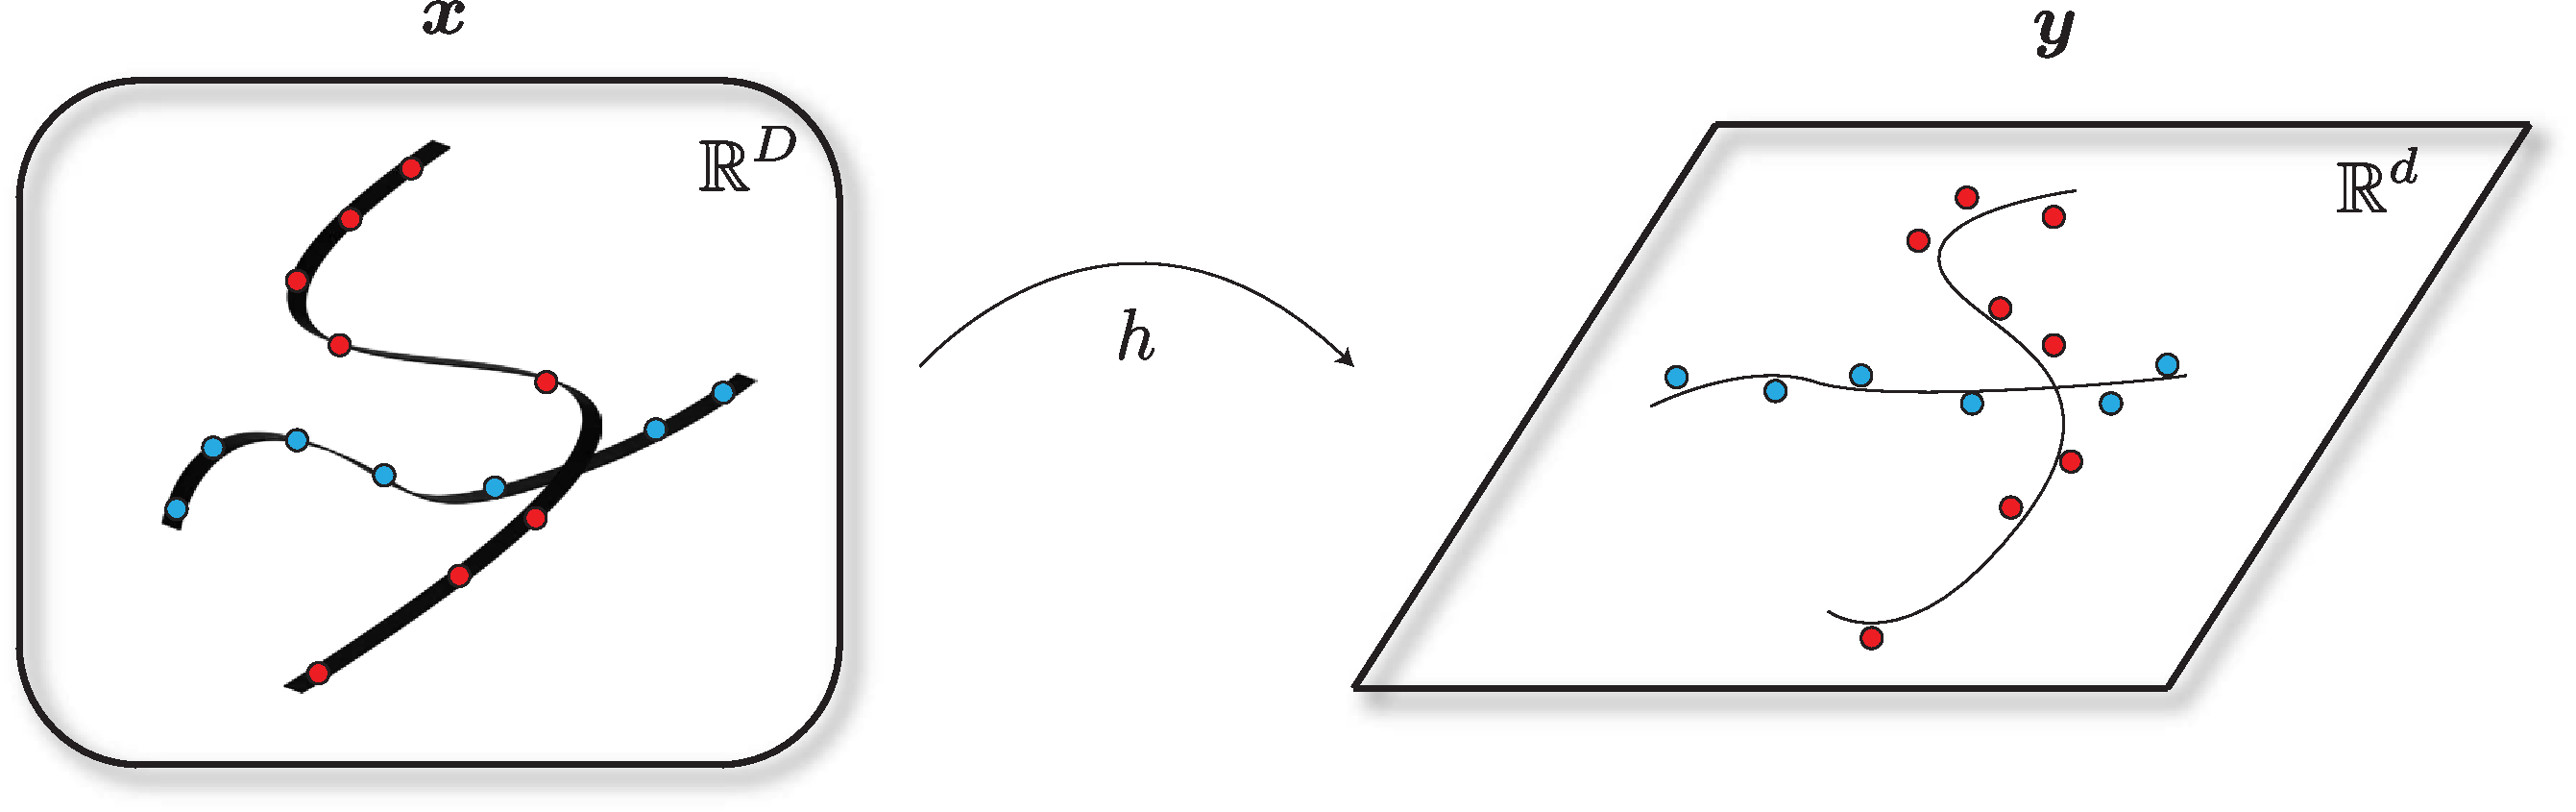
\includegraphics[width=0.9\textwidth]{\toplevelprefix/chapters/chapter6/figs/inference_roadmap.pdf}
  \caption{\small \textbf{基于低维分布的推断。} 这是本章的通用示意图:我们有一个关于\(\vx \in \R^{D}\)的低维分布(此处描绘为\(\R^{3}\)中两个二维流形的并集),以及一个测量模型\(\y = h(\vx) + \vw \in \R^{d}\)。我们希望推断关于此模型的各种信息,包括在给定\(\vy\)的条件下\(\vx\)的条件分布,或条件期望\(\mathbb{E}[\vx \mid \y]\),这些推断基于关于模型的各种信息以及(可能有限的)\(\vx\)或\(\vy\)的样本。}
  \label{fig:inference_roadmap}
\end{figure}

\begin{example}[图像补全与文本预测]
流行的自然图像补全和自然语言预测是两个典型任务,它们要求我们根据部分观测 $\y$ 恢复出完整的数据 $\x$,其中 $\x$ 的一部分被遮盖,需要根据其余部分来补全。图\ref{fig:image-text-completion}展示了这类任务的一些例子。事实上,正是这些任务启发了现代大型模型(如用于文本生成的GPT)和图像补全模型(如掩码自编码器)的训练方式,我们稍后将更详细地研究这些模型。
    \begin{figure}
        \centering
        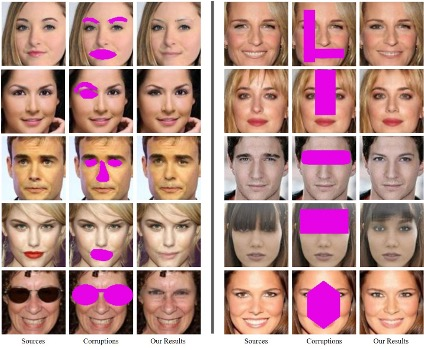
\includegraphics[height=0.4\linewidth]{\toplevelprefix/chapters/chapter6/figs/image-completion.jpg} \hspace{10mm} 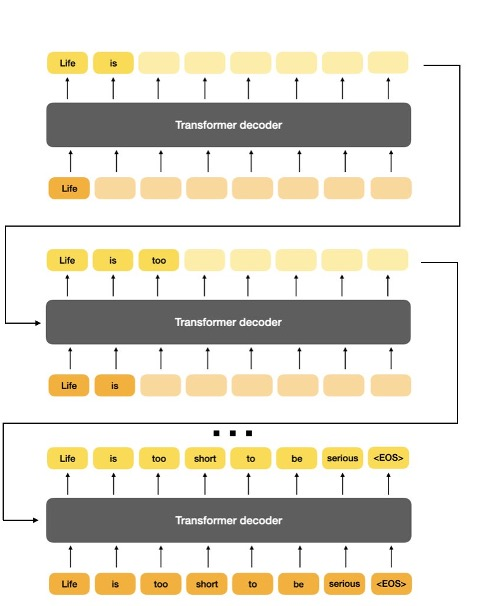
\includegraphics[height=0.45\linewidth]{\toplevelprefix/chapters/chapter6/figs/text-prediction.jpg}
        \caption{左图:图像补全。右图:文本预测。特别是,文本预测是流行的生成式预训练变换器(GPT)的灵感来源。}
        \label{fig:image-text-completion}
    \end{figure}
\end{example}


\paragraph{通过贝叶斯法则的统计学解释。}
总的来说,要出色地完成这类任务,我们需要掌握条件分布 $p(\x\mid \y)$。如果我们有了它,我们就能找到最大似然估计(预测):
\begin{equation}
  \hat{\x} = \argmax_{\x} p(\x\mid \y);
\end{equation}
计算条件期望估计:
\begin{equation}
  \hat{\x} = \mathbb{E}[\x \mid \y] = \int \x p(\x\mid \y)\odif{\vx};
\end{equation}
以及从条件分布中采样:
\begin{equation}
  \hat{\x} \sim p(\x \mid \y).
\end{equation}

注意到,根据贝叶斯法则,我们有
\begin{equation}
  p(\x\mid \y) = \frac{p(\y\mid \x) p(\x) }{p(\y)}.
\end{equation} 
例如,最大似然估计可以通过求解以下(最大对数似然)规划问题来计算:
\begin{equation}
    \hat{\x} = \argmax_{\x} [\log p(\y\mid \x) + \log p(\x)], 
\end{equation}
比如说通过梯度上升法:
\begin{equation}
    \x_{k+1} = \x_k + \alpha \cdot \big(\nabla_{\x} \log p(\y \mid \x) + \nabla_{\x} \log p(\x)\big).
    \label{eqn:loglikelihoo-gradient-ascent}
\end{equation}
高效地计算条件分布 $p(\x \mid \y)$ 自然取决于我们如何学习和利用数据 $\x$ 的低维分布 $p(\x)$ 以及决定了条件分布 $p(\y \mid \x)$ 的观测模型 $\y = h(\x) + \vw$。

\paragraph{作为约束优化的几何解释。}

由于\(\vx\)分布的支撑集\(\cS_{\vx}\)是低维的,我们可以假设存在一个函数\(F\),使得
\begin{equation}
  F(\vx) = \boldsymbol{0} \qquad \iff \qquad \vx \in \cS_{\vx}
\end{equation}
这样,\(\cS_{\vx} = F^{-1}(\{\vzero\})\) 就是分布 $p(\x)$ 的低维支撑集。从几何角度看,$F(\x)$ 的一个自然选择是到支撑集 $\mathcal{S}_{\x}$ 的“距离函数”:\footnote{请注意,在现实中,我们只有分布支撑集上的离散样本。本着在第\ref{ch:compression}章中研究的扩散或有损编码的连续化精神,我们可以将距离函数近似为 $    F(\x) \approx \min_{\x_p \in \cC_{\vx}^{\epsilon}} \|\x - \x_p\|_2$,其中 $\mathcal{S}_{\x}$ 被样本的一个$\epsilon$-球覆盖\(\cC_{\vx}^{\epsilon}\)所替代。}
\begin{equation}
    F(\x) = \min_{\x_p \in \mathcal{S}_{\x}} \|\x - \x_p\|_2. 
\end{equation}
现在给定 $\y = h(\x) +\vw$,为了求解 $\x$,我们可以解决以下约束优化问题:
\begin{equation}
    \max_{\x} - \frac{1}{2}\|h(\x) - \y\|_2^2 \quad \mbox{s.t.} \quad F(\x) = \boldsymbol{0}. 
\end{equation}
使用增广拉格朗日乘子法,我们可以求解以下无约束规划问题:
\begin{equation}
   \max_{\x} \left[-\frac{1}{2}\|h(\x) - \y\|_2^2  + \vlambda^{\top} F(\x) - \frac{\mu}{2} \|F(\x)\|_2^2\right]
\end{equation}
其中 $\vlambda$ 是某个常数拉格朗日乘子。
这等价于以下规划问题:
\begin{equation}\label{eq:lagrange_multiplier_continuation}
\max_{\x} \left[\log \exp\Big(- \frac{1}{2}\|h(\x) - \y\|_2^2\Big) + \log \exp\Big( - \frac{\mu}{2} \big\|F(\x) - \vlambda/\mu\big\|_2^2\Big)\right],
\end{equation} 
其中 $\vc \doteq {\vlambda}/{\mu}$ 可以被看作是约束函数的“均值”。当通过连续化方法强制施加约束时,$\mu$ 会变得很大\footnote{本着\Cref{ch:compression}中连续化的精神,我们通过令\(\eps \to 0\)来获得分布的更好近似;在这里,我们令\(\mu \to \infty\)。更大的\(\mu\)值将约束\(F\)在最优点处取越来越小的值,这意味着最优点位于支撑集\(\cS_{\vx}\)的一个越来越小的邻域内。有趣的是,拉格朗日乘子理论暗示,在关于\(F\)和目标函数中其他项的某些良性条件下,我们只需使\(\mu\)足够大,就能确保在最优点处\(F(\vx) = \vzero\),这意味着在\textit{有限}的惩罚下,我们能得到对支撑集的\textit{完美}近似。总的来说,我们应该有这样的直觉:\(\mu\)扮演的角色与\(\epsilon^{-1}\)相同。},$\|\vc\|_2$ 会变得越来越小。

上述规划问题可以从两个不同角度来解释。首先,可以将第一项看作是给定 $\x$ 时 $\y$ 的条件概率,第二项看作是 $\x$ 的概率密度:
\begin{equation}
  p(\y\mid \x) \propto \exp\Big(- \frac{1}{2}\|h(\x) - \y\|_2^2\Big), \quad 
    p(\x) \propto \exp\Big( - \frac{\mu}{2}\|F(\x) - \vc\|_2^2\Big).
\end{equation} 
因此,求解逆问题的约束优化等价于使用上述概率密度进行贝叶斯推断。所以,通过梯度上升法求解上述规划问题 \eqref{eq:lagrange_multiplier_continuation} 等价于上述最大似然估计 \eqref{eqn:loglikelihoo-gradient-ascent},
其中梯度形式为:
\begin{equation}
   \nabla_{\x} \log p(\y \mid \x) + \nabla_{\x} \log p(\x)   =  \pdv{h}{\vx}(\vx)\big(\y - h(\x)\big) + \mu \pdv{F}{\vx}(\vx)\big(\vc - F(\x)\big),
\end{equation}
这里 $\pdv{h}{\vx}(\vx)$ 和 $\pdv{F}{\vx}(\vx)$ 分别是 $h(\x)$ 和 $F(\x)$ 的雅可比矩阵。

其次,请注意上述规划问题 \eqref{eq:lagrange_multiplier_continuation} 等价于:
\begin{equation}
\min_{\x} \frac{1}{2}\|h(\x) - \y\|_2^2 + \frac{\mu}{2} \big\|F(\x) - \vlambda/\mu\big\|_2^2,
\label{eqn:energy-minimization}
\end{equation} 
由于这两项显著的二次型形式,它们也可以被解释为某种“能量”函数。这种表述在机器学习文献中常被称为“能量最小化”。

% 注意,通过梯度上升法来强制约束 $F(\x) = \boldsymbol{0}$ 的增广拉格朗日乘子法,等价于使用贝叶斯法则、与概率密度 $p(\x)$ 相关的得分以及与条件概率密度 $p(\y\mid \x)$ 相关的得分(在 $\x$ 空间中)进行直接的梯度上升。\DP{我认为这部分有些多余?}
% 人们可以将其视为我们之前在\eqref{eqn:conditional-denoising-score}中发展的条件生成得分的几何解释。


\paragraph{几种代表性的实际推断设定。} 
然而在实践中,关于 $\x$ 的分布以及 $\x$ 和 $\y$ 之间关系的初始信息可以以多种不同的方式或形式给出。总的来说,它们大多可以分为以下四种情况,这些情况在概念上难度递增:
\begin{itemize}
\item {\em 情况1:} $\x$ 的分布模型和观测模型 $\y = h(\x)$ $(+ \boldsymbol{w})$ 都是已知的,甚至具有解析形式。这在许多经典的信号处理问题中是典型情况,例如信号去噪、我们在第\ref{ch:classic}章中看到的稀疏向量恢复问题,以及下文将介绍的低秩矩阵恢复问题。
\item {\em 情况2:} 我们没有分布模型,只有 $\x$ 的样本 $\X = \{\x_1, \ldots, \x_N\}$,而观测模型 $\y = h(\x)$ $ (+ \boldsymbol{w})$ 是已知的。\footnote{在文献中,这种设定有时被称为{\em 经验贝叶斯推断}。} $\x$ 的分布 $p(\x)$ 需要被学习,随后条件分布 $p(\x\mid \y)$ 也需要被学习。自然图像补全或自然语言补全(例如,BERT 和 GPT)是这类问题的典型例子。
\item {\em 情况3:} 我们只有成对的样本:$(\X, \Y) = \{ (\x_1, \y_1), \ldots, (\x_N, \y_N) \}$。$\x$ 和 $\y$ 的分布以及它们之间的关系 $h(\cdot)$ 都需要从这些成对样本数据中学习。例如,给定许多图像及其标题,学习进行文本条件的图像生成就是这样一个问题。
\item {\em 情况4:} 我们只有观测 $\y$ 的样本 $\Y = \{\y_1, \ldots, \y_N\}$,并且观测模型 $h(\cdot)$ 需要被知道,至少在某个参数族 $h(\cdot, \boldsymbol{\theta})$ 内。分布 $p(\x)$ 和 $p(\x \mid \y)$ 需要从根据 $\Y$ 估计出的 $\hat \x$ 中学习。例如,从一系列已校准或未校准的视图中学习渲染一个新视图就是这样一个问题。
\end{itemize}
在本章中,我们将讨论学习所需分布并解决这些情况下相关条件估计或生成问题的通用方法,通常会以一个代表性问题为例。在整个章节中,您应该牢记\Cref{fig:inference_roadmap}所示的框架。

% 从这里开始,我们将把讨论的重点转向特定的现代应用,在这些应用中,我们希望为特定的结构化数据分布(如图像、3D场景和人体姿态)学习有用的表示,并且我们对数据的某些结构化属性有\textit{先验}知识,例如部分观测、类别标签或文本标题。在这种情况下,现代实践是间接建立这种自编码:我们不是在 $\vx$ 和 $\vz$ 之间建立直接的编码器-解码器映射,而是寻求在 $\vx$ 和 $\vz$ 之间建立一种\textit{绑定}或映射,这使我们能够根据(\textit{先验}指定的)属性 $\vz$ 生成 $\vx$ 的样本,甚至能够根据数据样本 $\vx$ 生成这些属性。这种方法与我们在前一章中讨论的直接编码器-解码器自编码循环高度相关,\footnote{在许多情况下甚至将其用作一个基本单元,例如在条件扩散模型中使用VAE。}但它能实现远为令人印象深刻的应用,包括现代生成模型所有开创性的多模态能力。


% 在本章中,我们将讨论如何利用这种自编码表示来完成数据域中的补全任务:这是一般绑定形式主义中一个具有教学意义的特例。更精确地说,我们将研究如何利用(压缩)自编码来根据数据的部分观测来补全一个数据样本。我们还将研究根据数据的某些学习到的特征或属性进行条件化数据采样和生成。
% 在本章和下一章中,我们将展示如何应用这些方法,在日益通用和具有挑战性的设置下,学习许多实际数据的分布和表示,以促进许多真实任务。


\section{已知数据分布下的条件推断}
请注意,在我们前几章讨论的设定中,自编码网络被训练来重构随机向量 $\x$ 的一组样本。这将允许我们从学到的(低维)分布中重新生成样本。在实践中,一旦分布的低维性被给定或学到,就可以利用它来进行稳定鲁棒的恢复、补全或预测任务。也就是说,在相当温和的条件下,人们可以从 $\x$ 的高度压缩、部分、含噪声甚至损坏的测量中恢复 $\x$,这些测量形如:
\begin{equation}
    \y = h(\x) + \vw,
\end{equation}
其中 $\y$ 通常是 $\x$ 的一个观测,其维度远低于 $\x$,而 $\vw$ 可以是随机噪声甚至稀疏的严重损坏。这类问题在经典信号处理文献中已被广泛研究,针对的是如稀疏向量、低秩矩阵等低维结构。感兴趣的读者可以参阅\cite{Wright-Ma-2022}以获得关于此主题的完整论述。

在这里,为了将经典工作置于更通用的现代背景下,我们通过一个可以说是最简单的数据(特别是图像)补全任务来说明其基本思想和事实。也就是说,我们考虑当一个样本 $\x$ 的部分缺失(甚至损坏)时如何恢复它。我们希望仅从观测到的一小部分 $\x$ 来恢复或预测其余部分:
\begin{equation}
f: \mathcal{P}_{\Omega}(\x) \mapsto \hat{\x},
\end{equation}
其中 $\mathcal{P}_{\Omega}(\spcdot)$ 代表一个掩码操作(参见\Cref{fig:matrix-completion}的例子)。

在本节和下一节中,我们将在两种不同的场景下研究补全任务:一种是当我们感兴趣的数据 $\x$ 的分布是{\em 先验}给定的,甚至具有某种解析形式。这种情况在经典信号处理中普遍存在,其中信号的结构被假定是已知的,例如带限、稀疏或低秩。另一种是当只有 $\x$ 的原始样本可用,我们需要从这些样本中学习低维分布以便很好地解决补全任务。自然图像补全或视频帧预测等任务就属于这种情况。作为本章其余部分的先导,我们从最简单的图像补全情况开始:当待补全的图像可以很好地被建模为一个低秩矩阵时。稍后我们将转向日益通用的情况和更具挑战性的设定。

\paragraph{低秩矩阵补全。}  
当数据分布是低维且已知时,低秩{\em 矩阵补全}是数据补全的一个经典问题。考虑从所有秩为 $r$ 的矩阵空间中随机抽取一个矩阵样本 $\X_o = [\x_1, \ldots, \x_n] \in \mathbb{R}^{m\times n}$。通常,我们假设矩阵的秩为
\begin{equation}
\mbox{rank}(\X_o) = r < \min\{m, n\}.
\end{equation}
因此很明显,局部来看,所有秩为 $r$ 的矩阵空间,其内在维度远低于环境空间 $mn$ 的维度。

现在,令 $\Omega$ 表示矩阵 $\X_o$ 中已观测条目的索引集合。已观测的条目为:
\begin{equation}
\Y = \mathcal{P}_{\Omega}(\X_o).
\end{equation}
支撑在 $\Omega^c$ 上的其余条目是未观测或缺失的。问题是我们能否从 $\Y$ 中正确且高效地恢复 $\X$ 的缺失条目。图\ref{fig:matrix-completion}展示了补全这样一个矩阵的一个例子。
% \begin{figure}
%     \centering
%     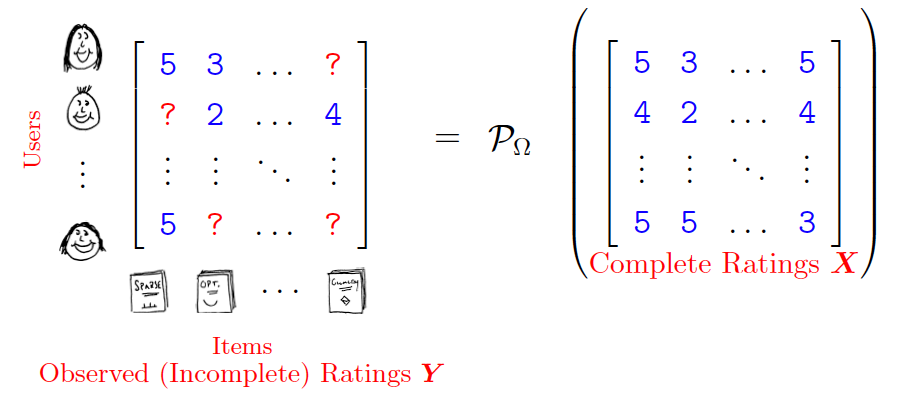
\includegraphics[width=0.8\linewidth]{\toplevelprefix/chapters/chapter6/figs/Matrix-Completion.png}
%     \caption{一个补全条目间具有相关性的矩阵的例子。}
%     \label{fig:matrix-completion}
% \end{figure}

\begin{figure}
\centering
% 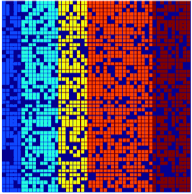
\includegraphics[width=0.3\linewidth]{\toplevelprefix/chapters/chapter6/figs/Matrix-masked.png}
% \hspace{5mm}  \hspace{5mm}
% 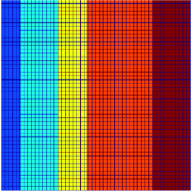
\includegraphics[width=0.3\linewidth]{\toplevelprefix/chapters/chapter6/figs/Matrix-completed.png}
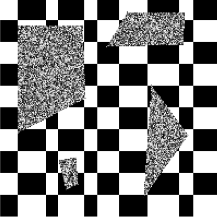
\includegraphics[width=0.3\linewidth]{\toplevelprefix/chapters/chapter6/figs/masked-checkerboard.png}\;\;
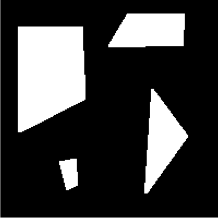
\includegraphics[width=0.3\linewidth]{\toplevelprefix/chapters/chapter6/figs/mask.png}\;\;
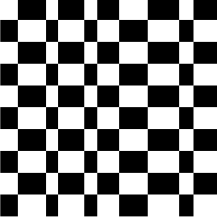
\includegraphics[width=0.3\linewidth]{\toplevelprefix/chapters/chapter6/figs/checkerboard.png}
\caption{将图像视为低秩矩阵并补全其部分被遮盖或损坏的条目的示意图。左图:被遮盖/损坏的图像 $\Y$;中图:掩码 $\Omega$;右图:补全后的图像 $\hat \X$。}
\label{fig:matrix-completion}
\end{figure}

请注意,这样一个矩阵之所以可以被补全,其根本原因在于矩阵的列和行高度相关,并且它们都位于一个低维子空间上。对于图\ref{fig:matrix-completion}中所示的例子,补全后矩阵的维度或秩仅为2。因此,恢复这样一个矩阵的基本思想是寻找一个在所有与观测条目一致的矩阵中秩最低的矩阵:
\begin{equation}
\min_{\X} \mbox{rank}(\X) \quad \mbox{subject to}
\quad
\Y = \mathcal{P}_{\Omega}(\X).
\label{eqn:rank-min}
\end{equation}
这被称为{\em 低秩矩阵补全}问题。关于所有低秩矩阵空间的完整刻画,请参见\cite{Wright-Ma-2022}。由于秩函数是不连续的,秩最小化通常是一个NP难问题,我们希望用一些更易于优化的东西来松弛它。

基于我们从第\ref{ch:compression}章学到的关于压缩的知识,我们可以通过强制使 $\X$ 中数据的有损编码率(或 $\X$ 所张成的体积)变小来促进恢复矩阵 $\X$ 的低秩性:
\begin{equation}
\min R_\epsilon(\X) = \frac{1}{2} \log \det \left(\boldsymbol{I} +
\alpha  \X\X^\top \right) \quad \mbox{subject to}
\quad
\Y = \mathcal{P}_{\Omega}(\X).
\label{eqn:rate-min}
\end{equation}
该问题可以被看作是上述低秩矩阵补全问题\eqref{eqn:rank-min}的一个连续松弛,并且可以通过梯度下降法求解。可以证明,针对 $\log\det$ 目标的梯度下降算子,恰好是在最小化矩阵 $\X\X^\top$ 秩的一个紧密代理。

率失真函数是一个非凸函数,其梯度下降并不总能保证找到全局最优解。然而,由于我们为 $\X$ 寻求的底层结构是分段线性的,秩函数有一个相当有效的凸松弛:核范数——即矩阵 $\X$ 所有奇异值的和。正如在压缩感知文献中所示,在相当广泛的条件下,\footnote{通常,这些条件规定了补全在计算上可行所必需的条目数量和充分性。这些条件已在\cite{Wright-Ma-2022}中被系统地刻画。}矩阵补全问题\eqref{eqn:rank-min}可以通过以下凸规划问题有效求解:
\begin{equation}
\min \|\X\|_* \quad \mbox{subject to}
\quad
\Y = \mathcal{P}_{\Omega}(\X),
\label{eqn:nuclear-min}
\end{equation}
其中核范数 $\|\X\|_*$ 是 $\X$ 的奇异值之和。在实践中,我们常常将上述约束凸优化问题转换为一个无约束问题:
\begin{equation}
\min \|\X\|_*  + \lambda \|
\Y - \mathcal{P}_{\Omega}(\X)\|_F^2,
\label{eqn:nuclear-min-lagrangian}
\end{equation}
对于某个适当选择的 $\lambda > 0$。感兴趣的读者可以参考\cite{Wright-Ma-2022}了解如何开发能够高效且有效地解决上述问题的算法。图\ref{fig:matrix-completion}展示了一个真实例子,其中矩阵 $\hat \X$ 实际上是通过求解上述规划问题恢复的。

\paragraph{进一步扩展。}
研究表明,具有低秩结构的图像(或更准确地说是纹理)和三维场景可以通过求解上述类型的优化问题非常有效地补全,即使存在额外的损坏和失真\cite{Zhang2010TILTTI,Liang-ECCV2012,Yi_2023_ICCV}:
\begin{equation}
    \Y \circ \tau = \X_o + \boldsymbol{E},
\end{equation}
其中 $\tau$ 是图像的某种未知非线性失真,$\boldsymbol{E}$ 是一个建模了某些(稀疏)遮挡和损坏的未知矩阵。同样,感兴趣的读者可以参考\cite{Wright-Ma-2022}以获得更详细的说明。

\section{基于已学得数据表示的条件推断}
在上一小节中,我们之所以能从部分观测 $\y$ 推断出 $\x$,是因为 $\X$ 的(支撑集)分布是{\em 先验}已知或指定的,例如所有低秩矩阵的集合。对于许多实际数据集,比如所有自然图像的集合,我们并没有像低秩矩阵那样具有解析形式的分布。然而,如果我们有足够的数据 $\x$ 的样本,我们应该能够首先学习其低维分布,然后利用它来进行基于观测 $\y = h(\x) + \vw$ 的未来推断任务。在本节中,我们假设观测模型 $h(\cdot)$ 是给定且已知的。我们将在下一节研究 $h(\cdot)$ 未被明确给出的情况。


\subsection{基于掩码自编码的图像补全}
对于一个通用图像 $\vX$,例如图\ref{fig:crate_mae_pipeline}左侧所示的图像,我们不能再将其视为一个低秩矩阵。然而,人类仍然表现出非凡的能力,即使在严重遮挡的情况下也能补全场景并识别熟悉的物体。这表明我们的大脑已经学习了自然图像的低维分布,并能用它来进行补全,进而进行识别。然而,所有自然图像的分布并不像低维线性子空间那样简单。因此,一个自然的问题是,我们能否学习自然图像更复杂的分布,并用它来执行图像补全任务?

\begin{figure}[t!]
%\vspace{-0.5in}
\begin{center}
  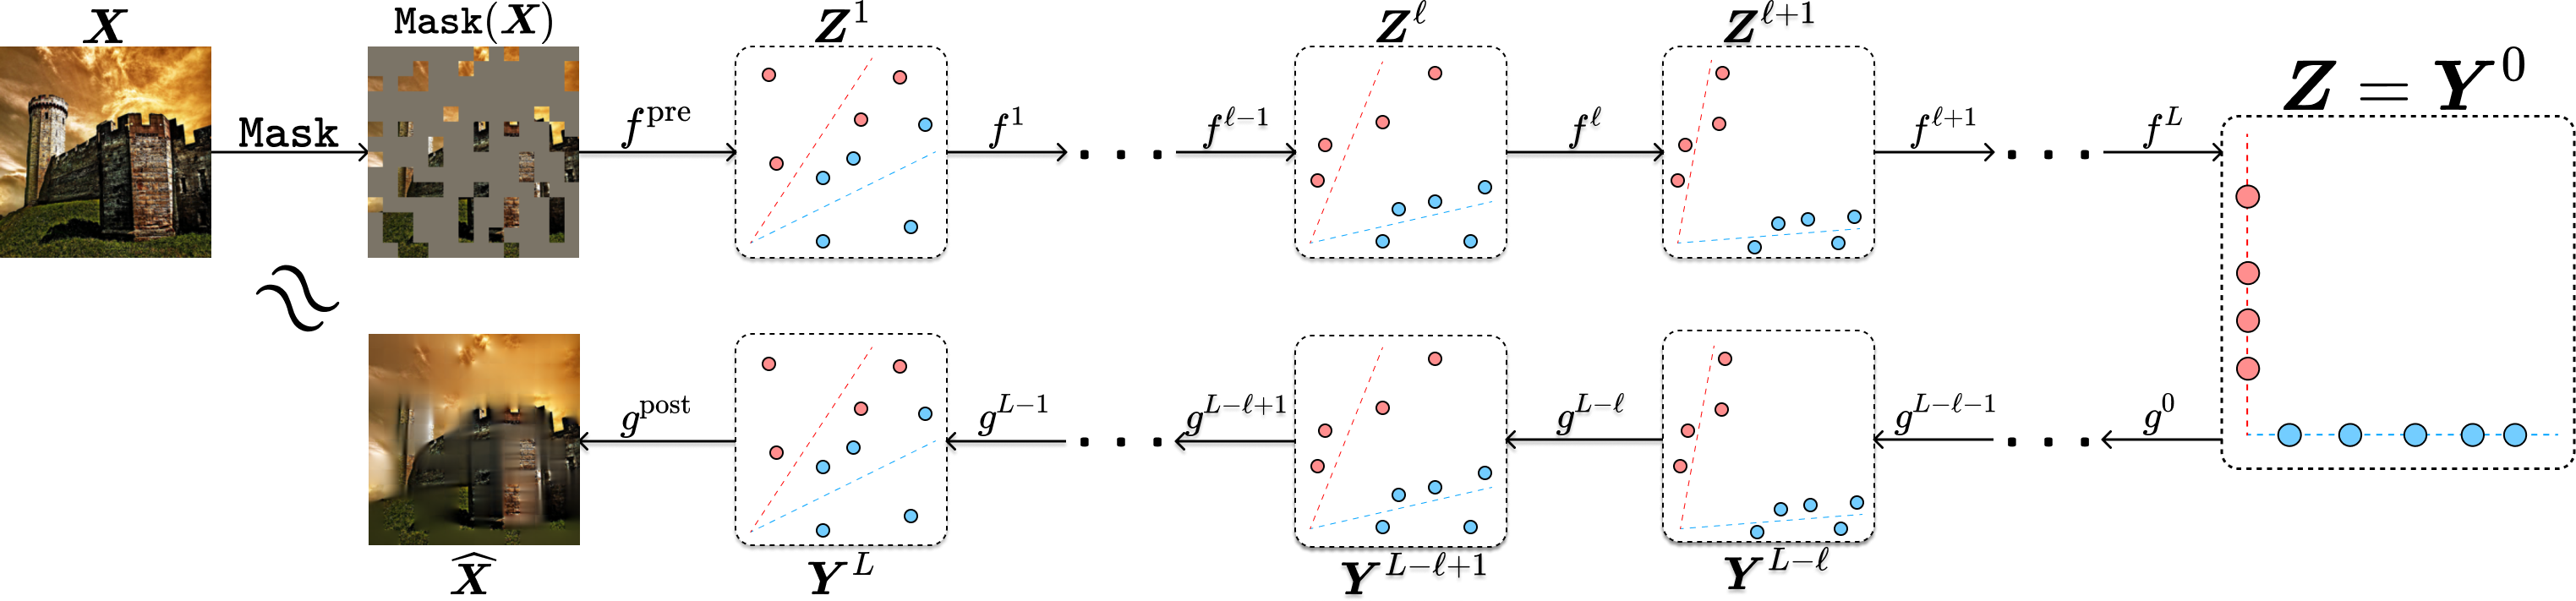
\includegraphics[width=0.99\textwidth]{\toplevelprefix/chapters/chapter6/figs/crate_mae_pipeline.png}
\end{center}
%\vspace{-0.1in}
\caption{\small \textbf{整体(掩码)自编码过程示意图。} (图像)令牌表示通过每个编码器层 \(f^{\ell}\) 被迭代地转换为一个简省的(例如,压缩和稀疏的)表示。此外,这些表示通过解码器层 \(g^{\ell}\) 被转换回原始图像。每个编码器层 \(f^{\ell}\) 旨在被相应的解码器层 \(g^{L - \ell}\)(部分地)逆转。}
\label{fig:crate_mae_pipeline}
%\vspace{-0.2in}
\end{figure}

图像补全任务的一种经验性方法是通过求解以下{\em 掩码自编码}(MAE)规划问题来找到一种编码和解码方案,该问题旨在最小化重构损失:
\begin{equation}\label{eq:mae_loss}
\min_{f, g} L_{\mathrm{MAE}}(f, g) \doteq \mathbb{E}\big[\norm{(g \circ
f)(\mathcal{P}_\Omega(\vX)) - \vX}_{2}^{2}].
\end{equation}
与具有简单底层结构的矩阵补全问题不同,我们不应再期望编码和解码映射具有简单的闭式形式,或者该规划问题可以通过显式算法求解。

对于一幅普通的自然图像,我们不能再假设其列或行是从一个低维子空间或一个低秩高斯分布中采样的。然而,一个合理的假设是图像由多个区域组成。每个区域内的图像块是相似的,可以被建模为一个(低秩)高斯分布或子空间。因此,为了利用分布的低维性,编码器 $f$ 的目标是将 $\X$ 转换为一个表示 $\Z$:
\begin{equation}
    f: \X \mapsto \Z
\end{equation}
使得 $\Z$ 的分布可以很好地被建模为子空间的混合,例如 $\{\vU_{[K]}\}$,从而在最小化稀疏性的同时最大化率缩减:
\begin{equation}\label{eq:sparse_rr}
\mathbb{E}_{\vZ = f(\vX)}[\Delta R_{\epsilon}(\vZ \mid \vU_{[K]}) - \lambda
\norm{\vZ}_{0}] = \mathbb{E}_{\vZ = f(\vX)}[R_\epsilon(\vZ) - R^{c}_\epsilon(\vZ \mid
\vU_{[K]}) - \lambda \norm{\vZ}_{0}],
\end{equation}
其中函数 $R_\epsilon(\cdot)$ 和 $R^c_\epsilon(\cdot)$ 分别在 \eqref{eq:coding_rate} 和 \eqref{eq:def-mcr-Rc} 中定义。

正如我们在前一章第\ref{ch:representation}章中所示,最小化上述目标的编码器 $f$ 可以由一系列类Transformer的算子构建。如\cite{Pai2024masked}的工作所示,解码器 $g$ 可以被视为并因此明确地构建为编码器 $f$ 的逆过程。图\ref{fig:crate_mae_layers}展示了每一层编码器和相应解码器的整体架构。编码器 $f$ 和解码器 $g$ 的参数可以通过梯度下降法优化重构损失\eqref{eq:mae_loss}来学习。

\begin{figure}[t!]
%\vspace{-0.5in}
\centering
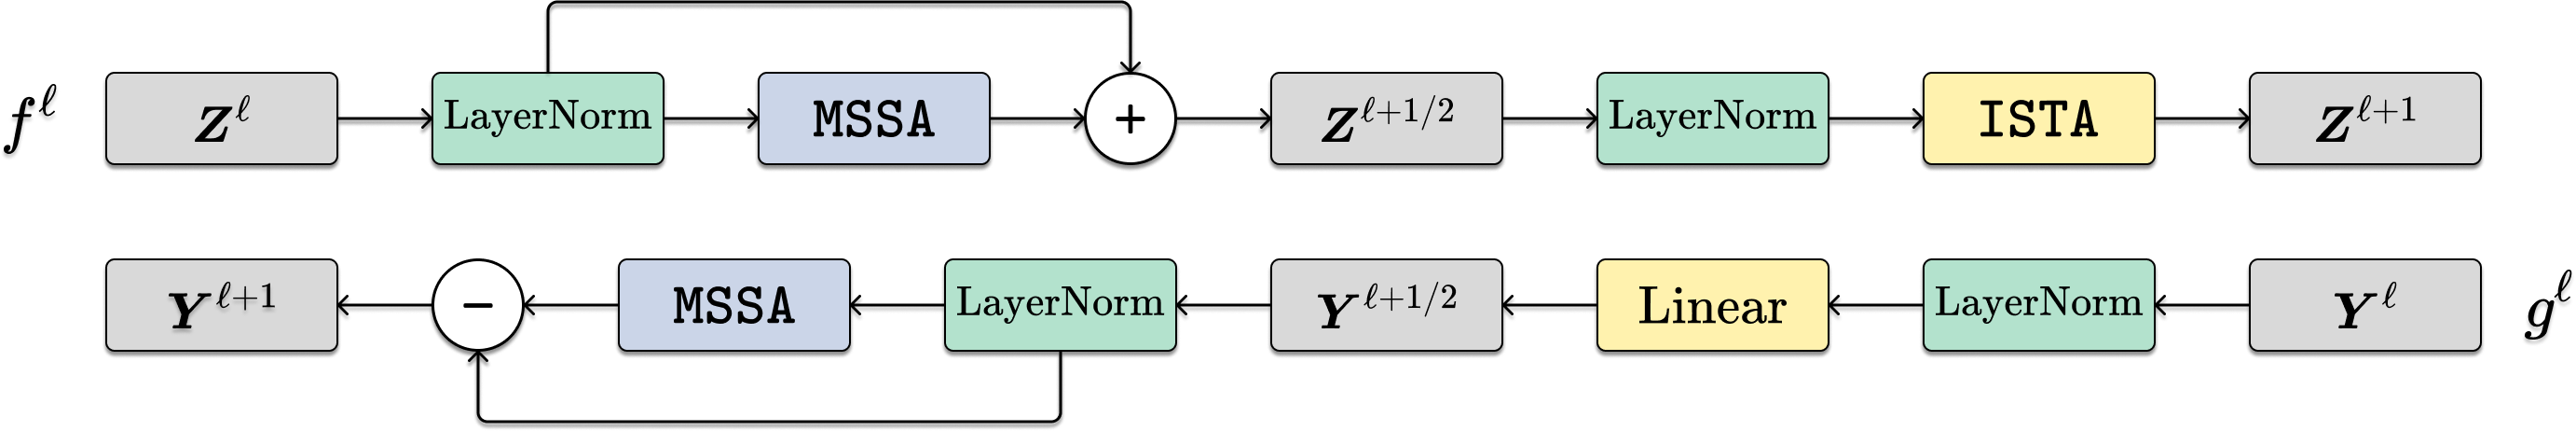
\includegraphics[width=0.99\textwidth]{\toplevelprefix/chapters/chapter6/figs/crate_mae_layers.png}
%\vspace{-0.1in}
\caption{\small \textbf{每个编码器层(\textit{顶部})和解码器层(\textit{底部})的示意图。} 请注意,这两层是高度反向平行的——每一层都被构建为以相反的顺序执行另一层的操作。也就是说,在解码器层 \(g^{\ell}\) 中,\(f^{L - \ell}\) 的 \(\ISTA\) 块首先使用一个线性层被部分地逆转,然后 \(f^{L - \ell}\) 的 \(\MSSA\) 块被逆转;这个顺序解开了在 \(f^{L - \ell}\) 中完成的变换。}
\label{fig:crate_mae_layers}
%\vspace{-0.2in}
\end{figure}

图\ref{fig:mae_autoencoding-small}展示了如此设计的掩码自编码器的一些代表性结果。关于自然图像补全的掩码自编码器的更多实现细节和结果可以在第\ref{ch:applications}章中找到。
\begin{figure}[t]
%\vspace{-0.5in}
\centering
\includegraphics[width=0.99\textwidth]{\toplevelprefix/chapters/chapter6/figs/crate_mae_autoencoding_small.pdf}
%\vspace{-0.1in}
\caption{\small \textbf{CRATE-Base 和 ViT-MAE-Base \cite{he2022masked} 在75\%图像块被掩码情况下的自编码可视化。} 我们观察到,尽管CRATE-Base使用的参数少于 ViT-MAE-Base 的 \(< 1/3\),但其重构效果与后者相当。
}
\label{fig:mae_autoencoding-small}
%\vspace{-0.2in}
\end{figure}

%\yima{将低秩矩阵补全推广到掩码自编码(MAE):\href{https://arxiv.org/abs/2404.02446}{掩码图像补全}。}

%\yima{或许可以尝试优化率缩减类型的目标... 理论依据:或许可以提及曲清组最近关于记忆和泛化的工作(针对PCA或低维高斯混合情况的扩散过程)。可能还有一些关于增量最优传输的工作...}

%\section{条件去噪与扩散}
%\label{sec:auto-denoising-diffusion}
%\yima{我们现在将逐样本重构的要求放宽到逐分布重构。}


\subsection{基于测量匹配的条件采样}
\label{sec:conditioned-decoding}
上述(掩码)自编码问题旨在生成一个与特定观测或条件一致的样本图像。但让我们更仔细地审视这种方法:给定图像的可见部分 $\X_v = \mathcal{P}_{\Omega}(\X)$,我们试图估计被掩码的部分 $\X_m = \mathcal{P}_{\Omega^c}(\X)$。对于随机变量 $\vX=(\vX_v, \vX_m)$ 的实现 $(\vXi_v, \vXi_m)$,令
\[p_{\X_m \mid \X_v}(\vXi_m\mid \vXi_v)\]
为给定 $\X_v$ 时 $\X_m$ 的条件分布。不难证明,MAE公式\eqref{eq:mae_loss}的最优解由条件期望给出:
\begin{equation}
  \argmin_{h = g \circ f}\, L_{\mathrm{MAE}}(h)
  % \doteq \mathbb{E}\big[\norm{(g \circ f)(\mathcal{P}_\Omega(\vX)) - \vX}_{2}^{2}].
  = \vXi_v \mapsto \vXi_v + \mathbb{E}[\X_m \mid \X_v=\vXi_v].
\end{equation}
然而,在一般情况下,这个期望甚至可能不落在自然图像的低维分布上!这部分解释了为什么\Cref{fig:mae_autoencoding-small}中一些恢复的图像块有些模糊。

对于许多实际目的,我们希望学习条件分布 $p_{\X_m \mid \X_v}$(或等价地,$p_{\X \mid \X_v}$)的(一个表示),然后直接从这个分布中获得一个清晰的(最可能的)样本。请注意,当 $\X$ 的分布是低维时,如果观测到 $\X$ 的一个足够大的部分 $\X_v$,它可能完全确定了 $\X$,从而也确定了缺失部分 $\X_m$。换句话说,分布 $p_{\X \mid \X_v}$ 是一个广义函数——如果 $\vX$ 完全由 $\vX_v$ 决定,它就是狄拉克δ函数,更一般地,是其某种奇异的变体。

因此,我们不应将补全任务作为条件估计问题来解决,而应将其作为条件采样问题来处理。为此,我们应首先学习所有自然图像 $\X$ 的(低维)分布。如果我们有足够多的自然图像样本,我们可以通过第\ref{ch:compression}章中描述的去噪过程 $\X_t$ 来学习该分布。然后,从部分观测 $\Y = \mathcal{P}_\Omega(\x) +\vw$ 中恢复 $\X$ 的问题就变成了一个条件生成问题——即在给定观测的条件下对分布进行采样。

\begin{figure}
  \centering
  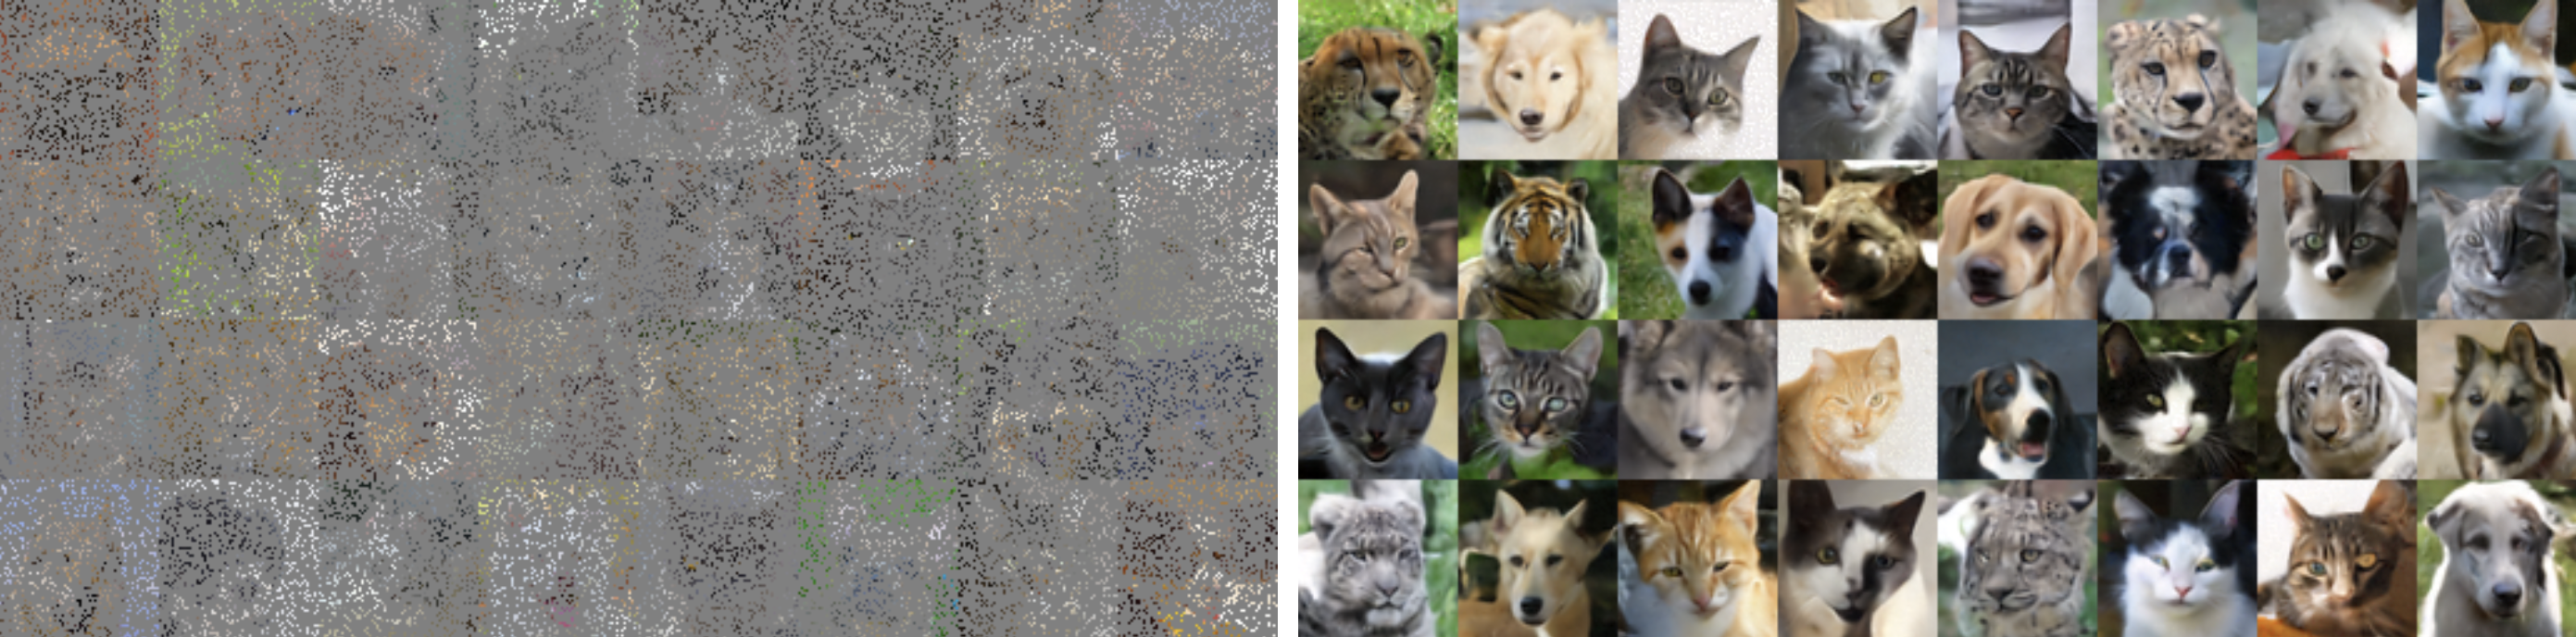
\includegraphics[width=1.0\textwidth]{\toplevelprefix/chapters/chapter6/figs/ambient_diffusion.png}
  \caption{\small \textbf{通过环境扩散(ambient diffusion)\cite{Daras-NIPS2023}训练的模型采样可视化,其中80\%的像素被遮盖。} 使用与\Cref{fig:mae_autoencoding-small}中相似的遮盖像素比例,环境扩散采样算法恢复的图像比基于MAE方法恢复的模糊图像要清晰得多。前者从自然图像的分布中采样,而后者近似于给定观测下该分布的条件期望(即平均值);这种平均化导致了模糊。}
  \label{fig:ambient_diffusion}
\end{figure}

\paragraph{一般线性测量。} 
事实上,我们甚至可以考虑从一个更一般的线性观测模型中恢复 $\X$:
\begin{equation}
    \Y = \vA\X_0,  \quad \X_t = \X_0 + \sigma_t \vG,  
\end{equation}
其中 $\vA$ 是矩阵空间上的一个线性算子\footnote{也就是说,如果我们想象将\(\vX\)展开成一个长向量,那么\(\vA\)就扮演了作用于\(\vX\)空间的一个矩阵的角色。},$\vG \sim \mathcal{N}(\boldsymbol{0}, \vI)$。图像补全任务中的掩码算子 $\mathcal{P}_{\Omega}(\cdot)$ 就是这种线性模型的一个例子。然后,\cite{daras2023ambient}已经证明
\begin{equation}
    \hat{\X}_* = \argmin_{\hat{\X}} \mathbb{E}[\|\vA(\hat{\X}(\vA\X_t, \vA) - \X_0)\|^2]
\end{equation}
满足以下条件:
\begin{equation}
    \vA \hat{\X}_*(\vA(\X_t), \vA) = \vA \mathbb{E}[\X_0 \mid \vA \X_t, \vA].
\end{equation} 
请注意,在 $\vA$ 是满列秩的特殊情况下,我们有 $ \mathbb{E}[\X_0 \mid \vA\X_t, \vA] = \mathbb{E}[\X_0 \mid \X_t]$。因此,在更一般的情况下,\cite{daras2023ambient}建议仍然可以使用如此获得的 $\mathbb{E}[\X_0 \mid \vA(\X_t), \vA]$ 来替代常规 $\X_t$ 去噪过程中的 $\mathbb{E}[\X_0 \mid \X_t]$:
\begin{equation}
    \X_{t-s} = \gamma_t \X_t + (1-\gamma_t) \mathbb{E}[\X_0 \mid \vA\X_t, \vA].
\end{equation}
这在实践中通常效果很好,例如对于许多图像修复任务,如\cite{daras2023ambient}所示。与从MAE恢复的模糊图像相比,通过上述方法恢复的图像要清晰得多,因为它利用了学到的自然图像分布,并从该分布中采样出一个与测量一致的(清晰)图像,如\Cref{fig:ambient_diffusion}所示(与\Cref{fig:mae_autoencoding-small}对比)。


\paragraph{一般非线性测量。}
为了推广上述(图像)补全问题并使之更严谨,我们可以考虑一个随机向量 $\vx \sim p$ 是通过一个更一般的观测函数被部分观测的:
\begin{equation}\label{eq:measurement-matching-observation}
\vy = h(\vx) + \vw,
\end{equation}
其中 $\vw$ 通常代表一些随机测量噪声,比如说高斯分布 $\vw \sim \mathcal{N}(\mathbf{0}, \sigma^2 \boldsymbol{I})$。不难看出,对于这样相关的 $\x$ 和 $\y$,如果噪声 $\vw$ 很小,它们的联合分布 $p(\x, \y)$ 自然是近乎退化的。在很大程度上,我们可以将 $p(\x, \y)$ 视为由函数 $\y = h(\x)$ 在联合空间 $(\x, \y)$ 中定义的超曲面的一个含噪版本。实际上,我们将考虑一种比纯矩阵补全更类似于掩码自编码的设定,即我们对于收到的每一个观测 $\vy$ 总能获得一个对应的干净样本 $\vx$。\footnote{在一些更专门的应用中,特别是在科学成像领域,能够在不接触任何干净/基准的 $\x$ 样本的情况下,学习从后验分布 $p_{\x \mid \y}$ 中生成样本是很有意义的。我们在本章末的注释中对该设定的方法进行了简要概述。}

与图像/矩阵补全类似,我们经常面临这样一种情况:$\vy$ 表示输入 $\vx$ 的一个退化或“有损”的观测。这可以以相当不同的形式表现出来。例如,在各种科学或医学成像问题中,测量数据 $\vy$ 可能是底层数据 $\vx$ 的一个压缩且损坏的观测;而在3D视觉任务中,$\vy$ 可能代表一个相机拍摄的物理对象的图像,该对象的姿态 $\vx$ 是未知的(但低维的)。通常,凭借数学建模(在某些情况下,还有测量系统的协同设计),我们知道 $h$ 并且可以在任何输入上对其进行评估,我们可以利用这一知识来帮助重构和采样 $\vx$。

\begin{figure}[t]
  \centering
  \begin{subfigure}{0.45\textwidth}
    \vspace{0.75cm}
    \centering
    \begin{tikzcd}[column sep=1.5cm]
      \vx \arrow[r, "h(\vx) + \vw"] & \vy \arrow[r, "p_{\vx \mid \vy}"]
      & \posteriorsample \arrow[r, "\posteriorsample + t\vg"] & \posteriorsample_t
    \end{tikzcd}
    \vspace{0.75cm}
    \caption{}
    \label{fig:left}
  \end{subfigure}
  \hfill
  \begin{subfigure}{0.45\textwidth}
    \centering
    \begin{tikzcd}[column sep=1.5cm, row sep=0.5cm]
    & \vy \\
    \vx \arrow[ur, "h(\vx) + \vw"] \arrow[dr, "\vx + t\vg"] & \\
    & \vx_t
    \end{tikzcd}
    \caption{}
    \label{fig:right}
  \end{subfigure}
  \caption{条件采样过程的统计依赖关系图。
  \textbf{左图:} 在将我们在\Cref{ch:compression}中发展的扩散-去噪方案直接(概念上)应用于条件采样时,我们使用来自后验分布 $p_{\vx \mid \vy}$ 的样本,直接在不同噪声水平的后验分布上训练去噪器,然后用它们来生成新样本。然而,在实践中,我们通常没有直接来自后验分布的样本,而是来自联合分布的成对样本 $(\vx, \vy)$。
  \textbf{右图:} 事实证明,仅需要对 $\vx$ 进行含噪观测就足以实现对应于 $p_{\posteriorsample_t \mid \posteriorsample}$ 的去噪器:这是因为在给定 $\vx$ 的条件下,$\vx_t$ 和 $\vy$ 是条件独立的。这意味着 $p_{\posteriorsample_t} = p_{\vx_t \mid \vy}$,这给出了一个用于去噪的得分函数,它由无条件得分函数和一个强制测量一致性的校正项组成。}
  \label{fig:posterior-sampling-cds}
\end{figure}


在技术层面,我们希望学到的数据表示能够帮助我们有效且高效地对条件分布 $p_{\vx\mid \vy}$(也称为后验分布)进行采样。更精确地说,用 $\vnu$ 表示随机变量 $\vy$ 的一个实现。我们希望生成样本 $\hat{\x}$ 使得:
\begin{equation}\label{eq:goal-sample-posterior}
  \hat{\x} \sim   p_{\vx \mid \y}(\spcdot \mid \vy=\vnu).
\end{equation}

回想一下,在\Cref{sub:compression_denoising}中,我们发展了一种自然而有效的方法来生成数据分布 $p$ 的\textit{无条件}样本。其要素是去噪器 $\bar{\x}^\ast(t, \vxi) = \bE[ \x \mid \vx_t=\vxi ]$,或其学到的近似 $\bar{\x}_{\theta}(t, \vxi)$,针对不同噪声水平的观测 $\x_t = \x + t \vg$(及其实现 $\vxi$),其中噪声为高斯噪声 $\vg \sim \cN(\mathbf{0}, \vI)$,且 $t \in [0, T]$,并选择了一系列时间点 $0 = t_1 < \hdots < t_{L} = T$ 来进行迭代去噪,从 $\hat{\vx}_{t_L} \sim \cN(\mathbf{0}, T^2 \vI)$ 开始(回顾\Cref{eq:denoising-iteration-basic})。\footnote{回顾我们在\Cref{sub:sampling_denoising}中的讨论,对这个基本的迭代去噪方案进行一些小的改进就足以带来有竞争力的实际性能。为了在发展条件采样时保持清晰,我们这里将关注最简单的实现。}
我们本可以直接应用这个方案来从后验分布 $p_{\vx \mid \vy}$ 生成样本,\textit{如果}我们对于 $\vy$ 的每个实现 $\vnu$ 都能访问一个样本数据集 $\posteriorsample \sim p_{\vx \mid \y}(\spcdot \mid \vnu)$,方法是生成含噪观测 $\posteriorsample_t$ 并训练去噪器来近似 $\bE[ \posteriorsample \mid \posteriorsample_t=\spcdot, \vy=\vnu ]$,即在含噪观测下后验分布的均值(见\Cref{fig:posterior-sampling-cds}(a))。然而,若仅有来自联合分布的成对样本 $(\vx, \vy)$,通过这种重采样(例如,通过对 $\vy$ 的值进行分箱)需要对高维数据而言多得令人望而却步的样本量,而其他方法则显式或隐式地依赖于密度估计,同样会遭受维度灾难。

幸运的是,事实证明这并非必要。考虑\Cref{fig:posterior-sampling-cds}(b)中的备选统计依赖图,它对应于通常的去噪-扩散过程中的随机变量,以及测量值 $\vy$。因为我们假设的观测模型\eqref{eq:measurement-matching-observation}意味着在给定 $\vx$ 的条件下,$\vx_t$ 和 $\vy$ 是独立的,所以对于 $\vy$ 的任何实现 $\vnu$,我们有
\begin{equation}\label{eq:conditional-denoising-conditioning-order-irrelevant}
  \begin{split}
  p_{\posteriorsample_t\mid \vy}(\spcdot \mid \vnu)
  &= \int
  \underbrace{p_{\posteriorsample_t \mid \posteriorsample}(\spcdot\mid \vxi)}_{=
  \cN(\vxi, t^2 \vI)}
  \spcdot \underbrace{p_{\posteriorsample \mid \vy}}_{= p_{\vx\mid \vy}}(\vxi \mid
  \vnu)
  \odif \vxi
  \\
  &=
  \int p_{\vx_t \mid \vx, \vy}(\spcdot\mid \vxi, \vnu) \spcdot p_{\vx \mid
  \vy}(\vxi\mid \vnu) \odif \vxi
  \\
  &=
  \int p_{\vx_t, \vx \mid \vy}(\spcdot, \vxi \mid \vnu) \odif \vxi
  \\
  &= p_{\vx_t \mid \vy}(\spcdot\mid \vnu).
  \end{split}
\end{equation}
在上述推导中,第一行识别了\Cref{fig:posterior-sampling-cds} (a,b)中出现的分布之间的等价性;第二行应用了这一点以及在给定 $\vx$ 的条件下 $\vx_t$ 和 $\vy$ 的条件独立性;第三行使用了条件概率的定义;最后一行对 $\vx$ 进行了边缘化。
因此,来自概念性后验采样过程的去噪器等于 $\bE[\vx \mid \vx_t=\spcdot, \vy=\vnu]$,这是我们可以仅从成对样本 $(\vx, \vy)$ 中学到的,
% 并且关于 $\vx_t$ 和 $\vy$ 的后验分布可以用贝叶斯法则表示为
% \begin{equation}
%   p(\vx \mid \vx_t, \vy) = \frac{p(\vx_t \mid \vx) p(\vx \mid \vy)}{p(\vx_t \mid
%   \vy)},
% \end{equation}
% 这里我们利用了 $\vx_t$ 在给定 $\vx$ 的条件下是独立高斯的。
并且根据特威迪公式(\Cref{thm:tweedie}),我们可以用 $p_{\vx_t \mid \vy}$ 的得分函数来表示这些去噪器,根据贝叶斯法则,该得分函数满足
\begin{equation}
  p_{\vx_t \mid \vy}(\vxi \mid \vnu) 
  = \frac{p_{\vy \mid \vx_t}(\vnu \mid \vxi) p_{\vx_t}(\vxi)}{p_{\vy}(\vnu)}.
\end{equation}
回想一下,$\vx_t$ 的密度由 $p_t = \varphi_{t} \ast p$ 给出,其中 $\varphi_{t}$ 表示均值为零、协方差为 $t^2 \vI$ 的标准高斯密度,$\ast$ 表示卷积。这正是我们从\Cref{sub:compression_denoising}中发展的标准扩散训练中得到的\textit{无条件得分函数}!
于是,条件得分函数对于 $(\vx_t, \vy)$ 的任何实现 $(\vxi, \vnu)$ 都满足
\begin{equation}
  \nabla_{\vxi} \log p_{\vx_t \mid \vy}(\vxi\mid \vnu)
  =
  \underbrace{\nabla_{\vxi} \log p_t(\vxi)}_{\text{得分匹配}}
  +
  \underbrace{\nabla_{\vxi} \log p_{\vy \mid \vx_t}(\vnu \mid \vxi)}_{\text{测量匹配}},
  \label{eqn:conditional-denoising-score}
\end{equation}
(通过特威迪公式)给出我们提出的去噪器为
\begin{align*}
  \bE[ \vx \mid \vx_t=\vxi, \vy=\vnu]
  &=
  \vxi + t^2 \nabla_{\vxi}\log p_t(\vxi) + t^2 \nabla_{\vxi}\log p_{\vy \mid
  \vx_t}(\vnu \mid \vxi)
  \\
  &=
  \bE[\vx \mid \vx_t=\vxi] + t^2 \nabla_{\vxi}\log p_{\vy \mid \vx_t}(\vnu\mid
  \vxi).
  \labelthis \label{eq:posterior-sampling-denoiser-decomposition}
\end{align*}
得到的算子可以解释为对含噪观测的无条件去噪器的一个\textit{校正}版本,其中校正项(即所谓的“测量匹配”项)强制与观测 $\vy$ 保持一致。读者应注意上述得分函数中梯度算子作用于哪个参数,以便完全掌握该算子的含义。
\yima{我们是否可以直接用测量约束 $\|\y - h(\x_t)\|^2$ 替换 $\log p(\y \mid \x_t)$,并用其梯度替换上述方程中的第二项?} \DP{这要求 \(y \mid \vx_{t}\) 类似于 \(\dNorm(\vy; h(\vx_{t}), \sigma{2}\vI)\),其中 \(1/\sigma^{2}\) 最终成为学习率。这个假设可以陈述,但我认为有点不切实际。}

要使这个过程在计算上可行,剩下的关键问题是如何计算测量匹配校正项,因为通常我们没有似然函数 $p_{\vy \mid \vx_t}$ 的闭式表达式,除非当 $t=0$ 时。在处理这个问题之前,我们讨论一个说明性的具体例子,延续我们在\Cref{sub:compression_denoising}中发展的例子。

\begin{example}\label{example:denoising-conditional-gaussian}
  考虑数据分布为高斯分布,均值为 $\vmu \in \bR^D$,协方差为 $\vSigma \in \bR^{D \times D}$,即 $\vx \sim \cN(\vmu, \vSigma)$。假设 $\vSigma \succeq \Zero$ 且非零。此外,在测量模型\eqref{eq:measurement-matching-observation}中,假设我们获得 $\vx$ 的线性测量,并带有独立高斯噪声,其中 $\vA \in \bR^{d \times D}$ 且 $\vy = \vA \vx + \sigma \vw$,其中 $\vw \sim \cN(\Zero, \vI)$ 且与 $\vx$ 独立。
  那么 $\vx =_{d} \vSigma^{1/2} \vg + \vmu$,其中 $\vg \sim \cN(\Zero, \vI)$ 与 $\vw$ 独立,$\vSigma^{1/2}$ 是协方差矩阵 $\vSigma$ 的唯一正平方根。经过一番代数运算,我们可以写出
  \begin{equation*}
    \begin{bmatrix}
      \vx \\
      \vy
    \end{bmatrix}
    =_{d}
    \begin{bmatrix}
      \vSigma^{1/2} & \Zero \\
      \vA \vSigma^{1/2} & \sigma \vI
    \end{bmatrix}
    \begin{bmatrix}
      \vg \\
      \vw
    \end{bmatrix}
    +
    \begin{bmatrix}
      \vmu \\
      \vA\vmu
    \end{bmatrix}.
  \end{equation*}
  根据独立性,我们有 $(\vg, \vw)$ 是联合高斯分布,这意味着 $(\vx, \vy)$ 也是联合高斯分布,因为它是联合高斯向量的仿射像。其协方差矩阵为
  \begin{equation*}
    \begin{bmatrix}
      \vSigma^{1/2} & \Zero \\
      \vA \vSigma^{1/2} & \sigma \vI
    \end{bmatrix}
    \begin{bmatrix}
      \vSigma^{1/2} & \Zero \\
      \vA \vSigma^{1/2} & \sigma \vI
    \end{bmatrix}^\top
    =
    \begin{bmatrix}
      \vSigma & \vSigma \vA^\top \\
      \vA \vSigma & \vA \vSigma \vA^\top + \sigma^2 \vI
    \end{bmatrix}.
  \end{equation*}
  现在,我们应用一个事实:对一个联合高斯分布的随机向量,以其部分坐标为条件,得到的仍然是一个高斯分布(\Cref{exercise:conditional_gaussian})。由此,我们得到
  \begin{equation}
    p_{\x \mid \y}(\spcdot \mid \vnu) = \cN\left(
    \underbrace{%
      \vmu + \vSigma\vA^\top \left(\vA\vSigma\vA^\top + \sigma^2 \vI\right)^{-1} 
      (\vnu - \vA\vmu)}_{\vmu_{\vx \mid \vy}(\vnu)},
      \underbrace{%
      \vSigma - \vSigma \vA^\top \left(\vA\vSigma\vA^\top + \sigma^2
      \vI\right)^{-1} \vA \vSigma}_{\vSigma_{\vx\mid \vy}}
    \right).
  \end{equation}
  根据我们上面推导的等价性,通过再次应用\Cref{exercise:conditional_gaussian},我们得到
  \begin{equation}\label{eq:conditional-posterior-denoiser-gaussian-case}
    \bE[ \vx \mid \vx_t=\vxi, \vy=\vnu ]
    =
    \vmu_{\vx\mid \vy}(\vnu) + \vSigma_{\vx\mid\vy}\left(
    \vSigma_{\vx\mid \vy} + t^2 \vI 
    \right)^{-1}\left(
    \vxi - \vmu_{\vx\mid \vy}(\vnu)
    \right).
  \end{equation}
  这个去噪器的函数形式相当简单,但它对问题数据 $\vmu$、$\vSigma$、$\vA$ 和 $\sigma^2$ 有着繁琐的依赖。我们可以通过与\Cref{eq:posterior-sampling-denoiser-decomposition}进行比较来进一步洞察其行为。我们像往常一样有
  \begin{equation}\label{eq:posterior-denoiser-gaussian-case}
    \bE[\vx \mid \vx_t=\vxi]
    = \vmu + \vSigma\left(\vSigma + t^2 \vI\right)^{-1} (\vxi - \vmu),
  \end{equation}
  这相当简单——这表明测量匹配项相当复杂。为了证实这一点,我们可以直接使用 $(\vx_t, \vy)$ 的联合分布表达式来计算似然 $p_{\vy \mid \vx_t}$:
  \begin{equation}
    \begin{bmatrix}
      \vx \\
      \vx_t \\
      \vy
    \end{bmatrix}
    =_{d}
    \begin{bmatrix}
      \vSigma^{1/2} & \Zero & \Zero \\
      \vSigma^{1/2} & t\vI & \Zero \\
      \vA \vSigma^{1/2} & \Zero & \sigma \vI
    \end{bmatrix}
    \begin{bmatrix}
      \vg \\
      \vg' \\
      \vw
    \end{bmatrix}
    +
    \begin{bmatrix}
      \vmu \\
      \vmu \\
      \vA\vmu
    \end{bmatrix},
  \end{equation}
  其中 $\vg' \sim \cN(\Zero, \vI)$ 且与其他高斯变量独立。这又是一个联合高斯分布;仅限制在最后两行,我们有协方差
  \begin{equation*}
    \begin{bmatrix}
      \vSigma^{1/2} & t\vI & \Zero \\
      \vA \vSigma^{1/2} & \Zero & \sigma \vI
    \end{bmatrix}
    \begin{bmatrix}
      \vSigma^{1/2} & t\vI & \Zero \\
      \vA \vSigma^{1/2} & \Zero & \sigma \vI
    \end{bmatrix}^\top
    =
    \begin{bmatrix}
      \vSigma + t^2\vI & \vSigma\vA^\top \\
      \vA\vSigma & \vA\vSigma\vA^\top + \sigma^2 \vI
    \end{bmatrix}.
  \end{equation*}
  再次应用\Cref{exercise:conditional_gaussian},我们得到
  \begin{equation}
    p_{\y \mid \vx_t}(\spcdot \mid \vxi) = \cN\left(
    \underbrace{%
      \vA\vmu + \vA\vSigma\left( \vSigma + t^2 \vI \right)^{-1}
      \left(
        \vxi - \vmu
      \right)
      }_{\vmu_{\vy \mid \vx_t}(\vxi)},
      \underbrace{%
        \vA\vSigma\vA^\top + \sigma^2 \vI - \vA\vSigma \left( \vSigma
        + t^2 \vI\right)^{-1} \vSigma \vA^\top
      }_{\vSigma_{\vy\mid \vx_t}}
    \right).
  \end{equation}
  现在注意到 $\vmu_{\vy \mid \vx_t}(\vxi) = \vA \bE[\vx \mid \vx_t=\vxi]$。所以,根据链式法则,
  \begin{align*}
    t^2 \nabla_{\vxi} \log p_{\vy \mid \vx_t}(\vnu \mid \vxi)
    &=
    t^2 \nabla_{\vxi}\left[
      -\frac{1}{2}
      (\vnu - \vA \bE[\vx \mid \vx_t=\vxi])^\top
      \vSigma_{\vy \mid \vx_t}^{-1}
      (\vnu - \vA \bE[\vx \mid \vx_t=\vxi])
      \right]
    \\
    &= t^2 (\vSigma+t^2 \vI)^{-1}\vSigma\vA^\top\vSigma_{\vy \mid \vx_t}^{-1}\left(
    \vnu - \vA \bE[\vx \mid \vx_t=\vxi] \right).
    \labelthis
    \label{eq:conditional-posterior-measurementmatching-gaussian-case}
  \end{align*}
  这给了我们一个对条件后验去噪器\eqref{eq:conditional-posterior-denoiser-gaussian-case}更具解释性的分解:根据\Cref{eq:posterior-sampling-denoiser-decomposition},它是无条件后验去噪器\eqref{eq:posterior-denoiser-gaussian-case}和测量匹配项\eqref{eq:conditional-posterior-measurementmatching-gaussian-case}的和。我们可以进一步分析测量匹配项。注意到
  \begin{equation}
    \vSigma_{\vy \mid \vx_t}
    =
    \sigma^2 \vI + \vA\vSigma^{1/2} \left(
      \vI - \vSigma^{1/2}\left(
      \vSigma + t^2 \vI
      \right)^{-1}
      \vSigma^{1/2}
    \right)\vSigma\vA^\top.
  \end{equation}
  如果我们令 $\vSigma = \vV \vLambda \vV^\top$ 表示 $\vSigma$ 的一个特征值分解,其中 $(\vv_i)$ 是 $\vV$ 的列,我们可以进一步写出
  \begin{align}
    \vSigma^{1/2}\left(
    \vI - \vSigma^{1/2}\left(
    \vSigma + t^2 \vI
    \right)^{-1}
    \vSigma^{1/2}
    \right) \vSigma^{1/2}
    &=
    t^2 \vV \vLambda^{1/2}\left(
      \vLambda + t^2 \vI
    \right)^{-1}
    \vLambda^{1/2}
    \vV^\top
    \\
    &=
    t^2 \sum_{i=1}^D
    \frac{\lambda_i}{\lambda_i + t^2}
    \vv_i \vv_i\adj.
  \end{align}
  那么对于任何等于零的 $\vSigma$ 的特征值,对应的加项为零;并且,记 $\lambda_{\min}(\vSigma)$ 为 $\vSigma$ 的最小正特征值(根据假设,它至少有一个正特征值),我们有(在某种可以被精确量化的意义上)只要 $t \ll \sqrt{\lambda_{\min}(\vSigma)}$,就成立
  \begin{equation}
    \frac{\lambda_i t^2}{\lambda_i + t^2} \approx 0.
  \end{equation}
  所以,当 $t \ll \sqrt{\lambda_{\min}(\vSigma)}$ 时,我们有近似
  \begin{equation}
    \vSigma_{\vy \mid \vx_t} \approx \sigma^2 \vI.
  \end{equation}
  这个近似的右侧等于 $\vSigma_{\vy \mid \vx}$。所以我们继而有
  \begin{equation}
    \nabla_{\vxi} \log p_{\vy \mid \vx_t}(\vnu \mid \vxi)
    \approx
    \nabla_{\vxi} \log p_{\vy \mid \vx}(\vnu \mid \bE[\vx \mid \vx_t = \vxi]).
    \label{eq:conditional-posterior-measurementmatching-gaussian-case-dps-approx}
  \end{equation}

  \begin{figure}[tbp]
    \centering
    % Top row (3 images)
    \begin{subfigure}{0.32\textwidth}
      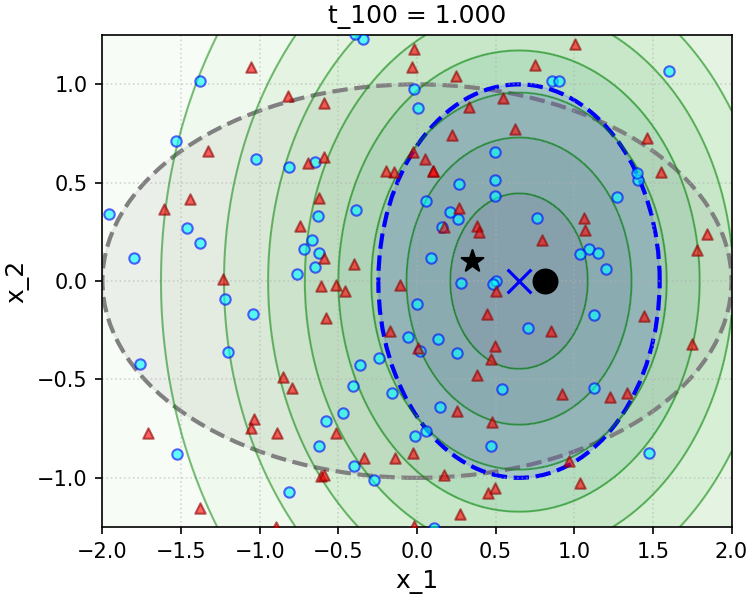
\includegraphics[width=\linewidth]{\toplevelprefix/chapters/chapter6/figs/samples_step_000_t_100_largenoise.png}
      % \caption{}
      % \label{}
    \end{subfigure}
    \hfill
    \begin{subfigure}{0.32\textwidth}
      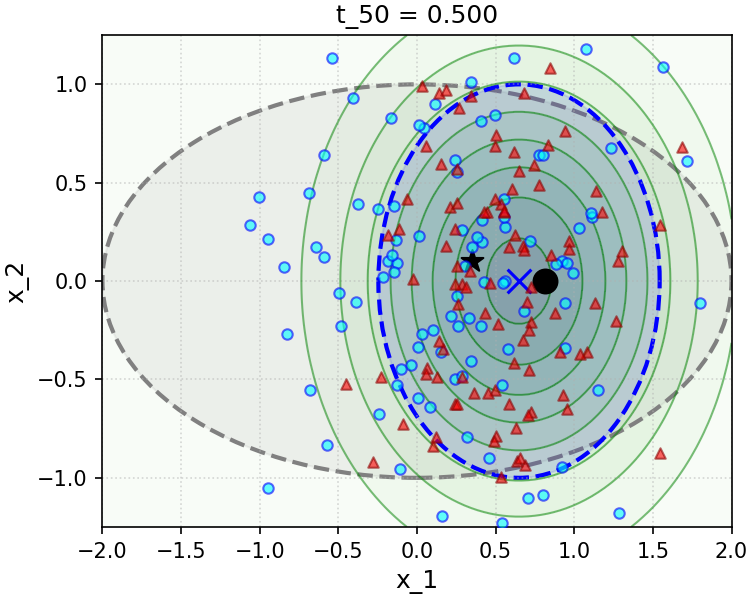
\includegraphics[width=\linewidth]{\toplevelprefix/chapters/chapter6/figs/samples_step_050_t_50_largenoise.png}
      % \caption{}
      % \label{}
    \end{subfigure}
    \hfill
    \begin{subfigure}{0.32\textwidth}
      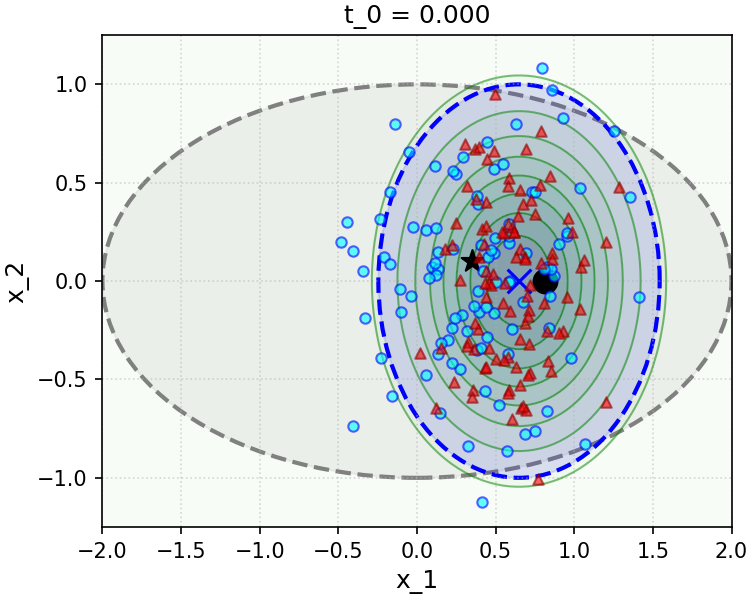
\includegraphics[width=\linewidth]{\toplevelprefix/chapters/chapter6/figs/samples_step_100_t_0_largenoise.png}
      % \caption{}
      % \label{}
    \end{subfigure}

    \vspace{2mm} % Add some vertical space between rows

    % Bottom row (3 images)
    \begin{subfigure}{0.32\textwidth}
      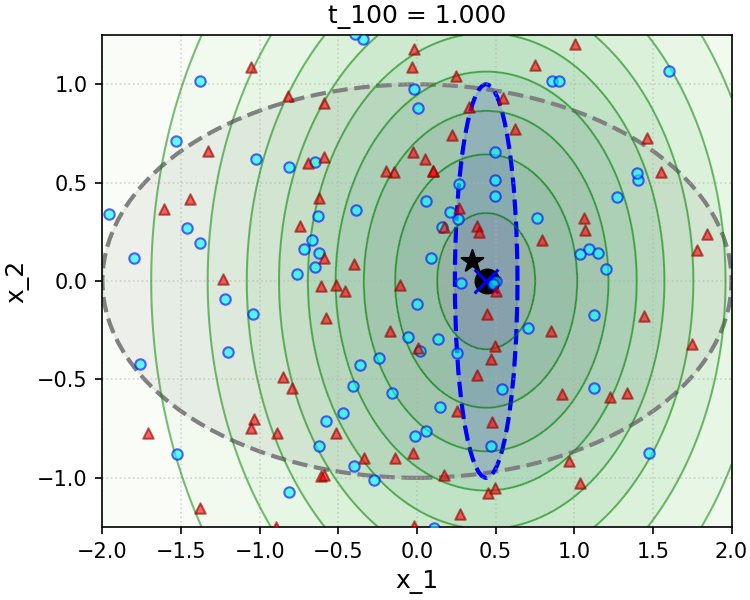
\includegraphics[width=\linewidth]{\toplevelprefix/chapters/chapter6/figs/samples_step_000_t_100_smallnoise.png}
      % \caption{}
      % \label{}
    \end{subfigure}
    \hfill
    \begin{subfigure}{0.32\textwidth}
      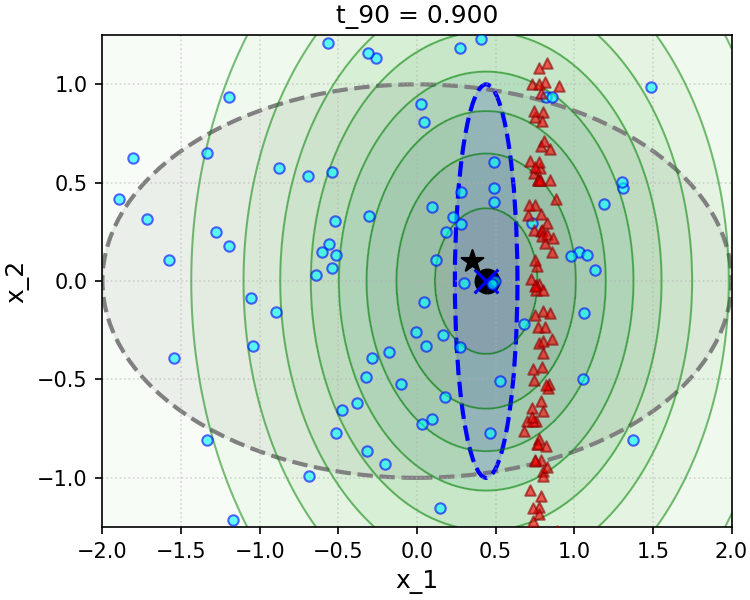
\includegraphics[width=\linewidth]{\toplevelprefix/chapters/chapter6/figs/samples_step_010_t_90_smallnoise.png}
      % \caption{}
      % \label{}
    \end{subfigure}
    \hfill
    \begin{subfigure}{0.32\textwidth}
      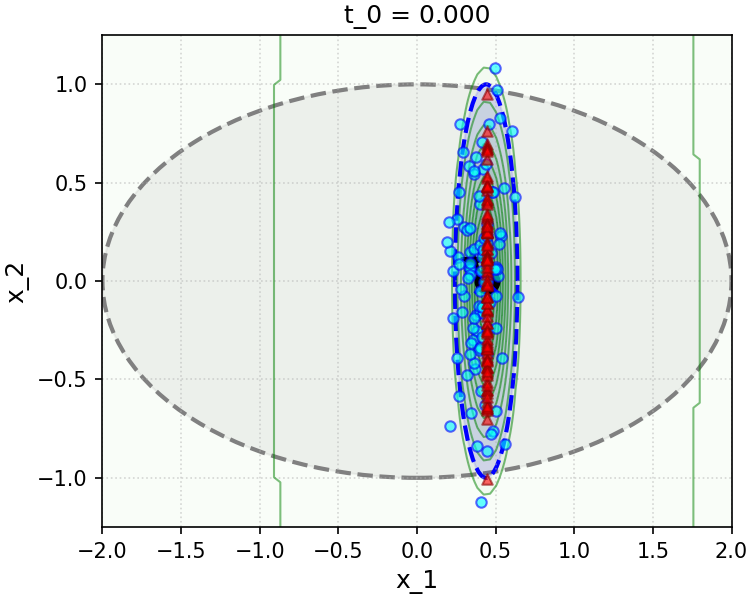
\includegraphics[width=\linewidth]{\toplevelprefix/chapters/chapter6/figs/samples_step_100_t_0_smallnoise.png}
      % \caption{}
      % \label{}
    \end{subfigure}

    \caption{条件采样设定\eqref{eq:measurement-matching-observation}的数值模拟,数据为高斯分布,测量为线性,噪声为高斯分布。我们模拟$D=2$和$d=1$,其中$\vSigma = \ve_1 \ve_1^\top + \tfrac{1}{4} \ve_2 \ve_2^\top$,$\vmu = \Zero$,以及$\vA = \ve_1^\top$。底层信号$\vx$用黑色星号标记,测量值$\vy$用黑色圆圈标记。每个单独的图对应于采样器时间$t_{\ell}$的不同值,不同行对应于不同的观测噪声水平$\sigma^2$。在每个图中,$\vx$的协方差矩阵用灰色绘制,$p_{\vx \mid \vy}$的后验协方差矩阵和后验均值用蓝色绘制(后验均值用蓝色“x”标记),$p_{\vx_{t_{\ell}} \mid \vy}$的等高线用绿色绘制。采样器超参数为$T=1$,$L=100$,我们抽取100个独立样本来初始化采样器。采样器使用在\Cref{example:denoising-conditional-gaussian}中推导的闭式去噪器实现,其中使用近似\eqref{eq:conditional-posterior-measurementmatching-gaussian-case-dps-approx}的用红色三角形标记,使用精确条件后验去噪器的用蓝色圆圈标记。
    \textbf{顶部:}对于较大的观测噪声$\sigma = 0.5$,精确的条件后验去噪器和近似的去噪器都能很好地收敛到后验分布$p_{\vx \mid \vy}$。采样时间(对应于“前向过程”中的时间,所以时间越大意味着噪声越大)从左到右递减。精确和近似的测量匹配项的收敛动态相似。
    \textbf{底部:}对于较小的观测噪声$\sigma = 0.1$,近似的测量匹配项导致采样器出现极端偏差(红色三角形):样本迅速收敛到一个仿射子空间,这些点与测量的基准值一致(除了来自后验均值去噪器的一些收缩),后续的采样迭代无法恢复沿该维度上丢失的后验方差。请注意,底部行绘制了与顶部行不同的时间$t_{\ell}$,以显示近似值沿测量维度向后验分布的快速坍缩。}
    \label{fig:conditional_sampling_computational_gaussian}
  \end{figure}

  \Cref{eq:conditional-posterior-measurementmatching-gaussian-case-dps-approx}当然是我们上述计算的直接结果。然而,请注意,如果我们直接解释这个近似,它\textit{从一开始}就是可计算的:似然函数 $p_{\vy \mid \vx} = \cN(\vA\vx, \sigma^2 \vI)$ 是一个以观测值为中心的简单高斯分布,我们得到的测量匹配项的近似可以被解释为简单地在条件期望 $\bE[\vx \mid \vx_t = \vxi]$ 处评估对数似然,然后对 $\vxi$ 求梯度(并通过条件期望进行反向传播,这里由\Cref{eq:posterior-denoiser-gaussian-case}给出)。然而,请注意\Cref{eq:conditional-posterior-measurementmatching-gaussian-case-dps-approx}中的近似要求 $t \ll \sqrt{\lambda_{\min}(\vSigma)}$,并且当这个条件不成立时,即使在这个高斯设定下,它通常也永远不准确。

  为了深入了解便捷近似\eqref{eq:conditional-posterior-measurementmatching-gaussian-case-dps-approx}的效果,我们在\Cref{fig:conditional_sampling_computational_gaussian}中实现并模拟了一个高斯设定下的简单数值实验。我们实现的采样器是我们在\Cref{ch:compression}中发展并在上面回顾的简单方案\eqref{eq:denoising-iteration-basic}的直接实现,使用了真实的条件后验去噪器,即\Cref{eq:conditional-posterior-denoiser-gaussian-case}(\Cref{fig:conditional_sampling_computational_gaussian}的顶行),以及利用分解\eqref{eq:posterior-sampling-denoiser-decomposition}、后验去噪器\eqref{eq:posterior-denoiser-gaussian-case}和测量匹配近似\eqref{eq:conditional-posterior-measurementmatching-gaussian-case-dps-approx}对该去噪器做的便捷近似(\Cref{fig:conditional_sampling_computational_gaussian}的底行)。我们看到,即使在简单的高斯设定下,我们对测量匹配项所做的近似也并非没有缺点——特别是在小噪声水平 $\sigma^2 \ll 1$ 时,它会导致采样分布的方差沿着与线性测量算子 $\vA$ 的行平行的方向迅速坍缩,这无法被后续的采样迭代所纠正。我们可以从近似\eqref{eq:conditional-posterior-measurementmatching-gaussian-case-dps-approx}和去噪迭代的定义\eqref{eq:denoising-iteration-basic}以及\Cref{eq:posterior-sampling-denoiser-decomposition}中直观地理解这一点:对于 $\sigma^2 \ll 1$,采样的早期步骤实际上是在似然函数上以非常大的步长进行梯度下降,通过\Cref{eq:conditional-posterior-measurementmatching-gaussian-case-dps-approx},这导致采样分布“卡”在一个坍缩的状态。

  % 另一方面,\Cref{fig:posterior-sampling-cds}中的第二个(更易于处理的)方案,涉及通过向$\vx$添加噪声来生成$\vx_t$,然后在之后对$\vy$进行条件化,会产生一个不同的联合分布
  % \begin{equation}
  %   \begin{bmatrix}
  %     \vx \\
  %     \vx_t \\
  %     \vy
  %   \end{bmatrix}
  %   =_{d}
  %   \begin{bmatrix}
  %     \vSigma^{1/2} & \Zero & \Zero \\
  %     \vSigma^{1/2} & t\vI & \Zero \\
  %     \vA \vSigma^{1/2} & \Zero & \sigma \vI
  %   \end{bmatrix}
  %   \begin{bmatrix}
  %     \vg \\
  %     \vg' \\
  %     \vw
  %   \end{bmatrix}
  %   +
  %   \begin{bmatrix}
  %     \vmu \\
  %     \vmu \\
  %     \vA\vmu
  %   \end{bmatrix},
  % \end{equation}
  % 其中 $\vg' \sim \cN(\Zero, \vI)$ 且与其他高斯变量独立。
  % 这又是一个联合高斯分布,其协方差为
  % \begin{equation*}
  %   \begin{bmatrix}
  %     \vSigma^{1/2} & \Zero & \Zero \\
  %     \vSigma^{1/2} & t\vI & \Zero \\
  %     \vA \vSigma^{1/2} & \Zero & \sigma \vI
  %   \end{bmatrix}
  %   \begin{bmatrix}
  %     \vSigma^{1/2} & \Zero & \Zero \\
  %     \vSigma^{1/2} & t\vI & \Zero \\
  %     \vA \vSigma^{1/2} & \Zero & \sigma \vI
  %   \end{bmatrix}^\top
  %   =
  %   \begin{bmatrix}
  %     \vSigma & \vSigma & \vSigma\vA^\top \\
  %     \vSigma & \vSigma + t^2\vI & \vSigma\vA^\top \\
  %     \vA \vSigma & \vA\vSigma & \vA\vSigma\vA^\top + \sigma^2 \vI
  %   \end{bmatrix}.
  % \end{equation*}
  % 再次使用\Cref{exercise:conditional_gaussian},我们推导出后验分布为
  % \begin{equation}
  %   p_{\vx \mid \vy, \vx_t}
  %   =
  %   \cN\left(
  %     ...
  %   \right)
  % \end{equation}
\end{example}


\Cref{example:denoising-conditional-gaussian}为测量匹配项\eqref{eq:conditional-posterior-measurementmatching-gaussian-case-dps-approx}提供了一个方便的近似,这个近似可以推广到该示例的高斯设定之外。为了在更普遍的情况下论证这个近似,注意到由于在给定 $\vx$ 的条件下 $\vy$ 和 $\vx_t$ 是条件独立的,我们可以写出
\begin{equation}
  p_{\vy \mid \vx_t}(\vnu \mid \vxi)
  =
  \int p_{\vy \mid \vx}(\vnu \mid \vxi') p_{\vx \mid \vx_t}(\vxi' \mid \vxi)
  \odif  \vxi'.
\end{equation}
形式上,当后验分布 $p_{\vx\mid \vx_t}$ 是一个以其均值 $\bE[\vx \mid \vx_t=\vxi]$ 为中心的狄拉克δ函数时,近似\eqref{eq:conditional-posterior-measurementmatching-gaussian-case-dps-approx}是精确的。更一般地,当后验分布 $p_{\vx \mid \vx_t}$ 高度集中于其均值附近时,近似\eqref{eq:conditional-posterior-measurementmatching-gaussian-case-dps-approx}是准确的。例如,对于足够小的 $t$ 这就成立,我们在\Cref{example:denoising-conditional-gaussian}的高斯设定中明确看到了这一点。
尽管\Cref{fig:conditional_sampling_computational_gaussian}中的数值模拟表明,这个近似在某些情况下并非没有弊端,但在实践中,它已被证明是一个可靠的基线,由Chung等人作为“扩散后验采样”(DPS)提出\cite{chung2023diffusion}。此外,甚至有原则性的、可推广的方法来改进它,通过整合更好的后验方差估计(这在\Cref{example:denoising-conditional-gaussian}的高斯设定中是精确的),我们将在本章末的总结中进一步讨论。

因此,借助DPS近似,我们通过\Cref{eq:posterior-sampling-denoiser-decomposition}得到了条件后验去噪器 $\bE[\vx \mid \vy, \vx_t]$ 的以下近似:
\begin{equation}
  \bE[ \vx \mid \vx_t=\vxi, \vy=\vnu]
  \approx
  \bE[\vx \mid \vx_t=\vxi] 
  + t^2 \nabla_{\vxi} \log p_{\vy \mid \vx}(\vnu \mid \bE[\vx \mid \vx_t = \vxi]).
  \label{eq:posterior-sampling-denoiser-decomposition-dps}
\end{equation}
并且,对于一个神经网络或其他模型 $\bar{\vx}_{\theta}(t, \vxi)$,它像在\Cref{sub:compression_denoising}中那样被训练来近似每个 $t \in [0, T]$ 的去噪器 $\bE[\vx \mid \vx_t = \vxi]$,我们得到了学到的条件后验去噪器
\begin{equation}
  \bar{\vx}_{\theta}(t, \vxi, \vnu) 
  = \bar{\vx}_{\theta}(t, \vxi)
  + t^2 \nabla_{\vxi} \log p_{\vy \mid \vx}(\vnu \mid \bar{\vx}_{\theta}(t,
  \vxi)).
  \label{eq:posterior-sampling-denoiser-learned-dps}
\end{equation}
请注意,近似\eqref{eq:posterior-sampling-denoiser-decomposition-dps}对于观测模型\eqref{eq:measurement-matching-observation}中任意的前向模型 $h$(包括非线性 $h$)都是有效的,甚至对于任何具有清晰似然函数 $p_{\vy \mid \vx}$ 表达式的噪声模型也有效。实际上,在有高斯噪声的情况下,我们有
\begin{equation}
  p_{\vy \mid \vx}(\vnu \mid \vxi)
  \propto
  \exp\left(
    -\frac{1}{2\sigma^2} \norm*{ h(\vxi) - \vnu }_2^2
  \right).
\end{equation}
因此,评估\eqref{eq:posterior-sampling-denoiser-learned-dps}的右侧仅需要
\begin{enumerate}
  \item 一个预训练的、针对数据分布 $p$($\vx$的分布)的去噪器 $\bar{\vx}_{\theta}(t, \vxi)$,如\Cref{sub:compression_denoising}中通过\Cref{alg:learning_denoiser}学习得到;
  \item 对测量模型\eqref{eq:measurement-matching-observation}的前向模型 $h$ 的前向和后向传播访问;
  \item 对 $\bar{\vx}_{\theta}(t, \vxi)$ 的一次前向和后向传播,这可以(例如)使用反向传播高效地评估。
\end{enumerate}

\begin{algorithm}
  \caption{在测量\eqref{eq:measurement-matching-observation}下的条件采样,使用无条件去噪器和DPS。}
	\label{alg:iterative_denoising_conditional_DPS}
	\begin{algorithmic}[1]
		\Require{一个用于采样的有序时间步长列表 \(0 \leq t_{0} < \cdots < t_{L} \leq T\)。}
    \Require{一个针对$p_{\vx}$的无条件去噪器 \(\bar{\vx}_{\theta} \colon \{t_{\ell}\}_{\ell = 1}^{L} \times \R^{D} \to \R^{D}\)。}
    \Require{要作为条件的$\vy$的测量实现$\vnu$(\Cref{eq:measurement-matching-observation})。}
    \Require{前向模型 $h : \bR^D \to \bR^d$ 和测量噪声方差 $\sigma^2 > 0$。}
		\Require{尺度和噪声水平函数 \(\alpha, \sigma \colon \{t_{\ell}\}_{\ell = 0}^{L} \to \R_{\geq 0}\)。}
    \Ensure{一个样本\(\hat{\vx}\),近似来自\(p_{\vx \mid \vy}\)。}
    \Function{DDIMSamplerConditionalDPS}{$\bar{\vx}_{\theta}, \vnu, h, \sigma^2, (t_{\ell})_{\ell = 0}^{L}$}
		\State{初始化 \(\hat{\vx}_{t_{L}} \sim\) \(\vx_{t_{L}}\)的近似分布} \Comment{VP \(\implies \dNorm(\vzero, \vI)\),VE \(\implies \dNorm(\vzero, t_{L}^{2}\vI)\)。}
		\For{\(\ell = L, L - 1, \dots, 1\)}
		% \State{计算
		% 	\begin{equation*}
  %       \nabla_{\vxi}\left[ -\frac{1}{2\sigma^2} \norm*{h(
  %       \bar{\vx}_{\theta}(t_{\ell}, \vxi)
  %       ) - \vnu}_2^2 \right]\biggl|_{\vxi = \hat{\vx}_{t_{\ell}}}\biggr.
		% 	\end{equation*}
		% }
		\State{计算
			\begin{equation*}
				\hat{\vx}_{t_{\ell - 1}} \doteq \frac{\sigma_{t_{\ell
        - 1}}}{\sigma_{t_{\ell}}}\hat{\vx}_{t_{\ell}} + \bp{\alpha_{t_{\ell
        - 1}} - \frac{\sigma_{t_{\ell
        - 1}}}{\sigma_{t_{\ell}}}\alpha_{t_{\ell}}}\left(
        \bar{\vx}_{\theta}(t_{\ell}, \hat{\vx}_{t_{\ell}})
        - \frac{\sigma_{t_{\ell}}^2}{2\alpha_{t_\ell}\sigma^2}
        \nabla_{\vxi}\left[ \norm*{h( \bar{\vx}_{\theta}(t_{\ell}, \vxi)
        ) - \vnu}_2^2 \right]\biggl|_{\vxi = \hat{\vx}_{t_{\ell}}}\biggr.
        \right)
			\end{equation*}
		}
		\EndFor
		\State{\Return{\(\hat{\vx}_{t_{0}}\)}}
		\EndFunction
	\end{algorithmic}
\end{algorithm}

将此方案与我们在\Cref{sub:compression_denoising}中发展的无条件采样基本实现相结合,我们得到了一个实用的算法,用于在给定遵循\eqref{eq:measurement-matching-observation}的测量条件下,对后验分布 $p_{\vx \mid \vy}$ 进行条件采样。\Cref{alg:iterative_denoising_conditional_DPS}记录了在已知标准差 $\sigma$ 的高斯观测噪声情况下的此方案,并稍作修改以扩展到一般的加噪过程,如\Cref{eq:gen_additive_gaussian_noise_model}及\Cref{ch:compression}中相关讨论所述(我们上面的讨论为了简化,选择了 $\alpha_t = 1$,$\sigma_t = t$,以及 $t_{\ell} = T\ell / L$,与\Cref{sub:compression_denoising}中的\Cref{eq:denoising-iteration-basic}一致)。



\subsection{以头部和手部为条件的身体姿态生成}\label{sub:ego-allo}
这类条件估计或生成问题在许多实际应用中非常自然地出现。一个典型的这类问题是如何在给定头部姿态和第一人称视角图像的条件下,估计和生成身体姿态和手势,如图\ref{fig:pose-teaser}所示。这通常是当人们佩戴头戴式设备,如苹果的Vision Pro或Meta的Project Aria时需要解决的问题。整个身体的姿态和手的姿势需要被推断出来,以便我们能用这些信息来控制人与之交互的虚拟对象。
\begin{figure*}[t]
  \centering
  \includegraphics[width=\linewidth]{\toplevelprefix/chapters/chapter6/figs/pose-teaser.pdf}
    \caption{
一个根据第一人称视角的SLAM姿态和图像(左图)来估计人体身高、姿态和手部参数(中图)的系统。输出捕捉了佩戴者在场景的异我参照系中的动作,我们在这里通过3D重建进行可视化(右图)。
  }
  \label{fig:pose-teaser}

\end{figure*}

请注意,在这种情况下,人们只能获得设备提供的头部姿态,以及对手部和上肢部分非常有限的视野。身体其余部分的姿态需要根据这些部分信息来“推断”或“补全”。唯一能够随时间估计身体姿态的方法是预先学习头部和身体姿态序列的联合分布,然后在给定实时部分输入的情况下对这个先验分布进行条件采样。图\ref{fig:pose-method}概述了一个名为EgoAllo \cite{yi2024egoallo}的系统,它基于一个学到的条件扩散-去噪模型来解决这个问题。
\begin{figure*}[t]
  \centering
  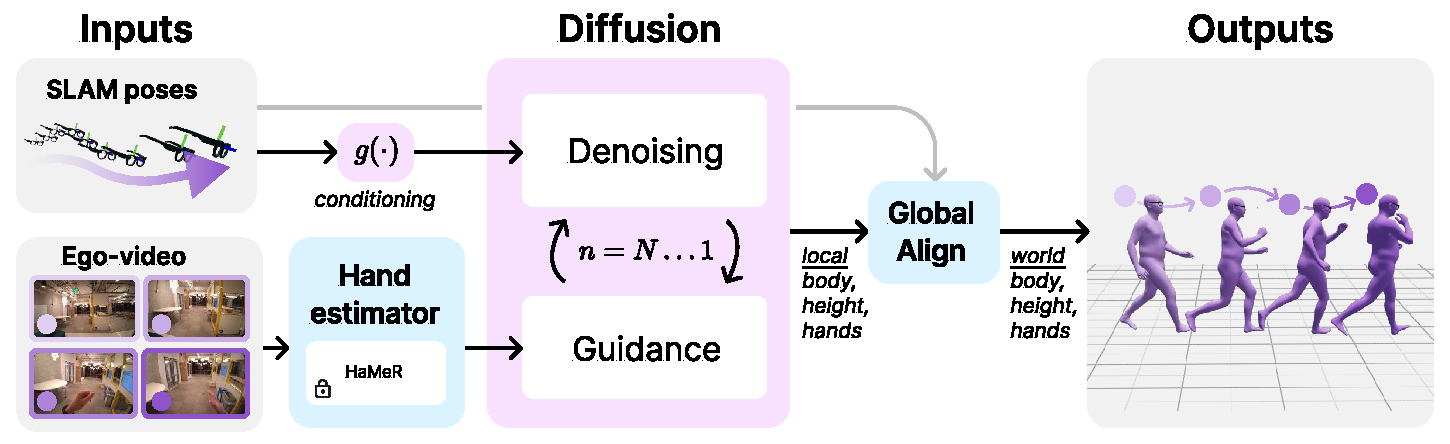
\includegraphics[width=\linewidth]{\toplevelprefix/chapters/chapter6/figs/pose-method.pdf}
\caption{
    \textbf{EgoAllo \cite{yi2024egoallo}技术组件概述。}
    % 我们以SLAM姿态和第一人称视角视频为输入。
    一个扩散模型被预训练,能够根据局部身体参数生成身体姿态序列(中图)。
    SLAM姿态的一个不变参数化$g(\cdot)$(左图)被用来对扩散模型进行条件化。这些参数可以通过全局对齐到输入姿态,从而被放置到全局坐标系中。
    当第一人称视角视频可用时,它被用于通过HaMeR~\cite{pavlakos2023reconstructing}进行手部检测(左图),这可以通过生成的手势进行引导,并融入到样本中。
  }
  \label{fig:pose-method}
\end{figure*}


图\ref{fig:comparison}比较了一些基准运动序列与EgoAllo生成的采样结果。尽管图中对每个输入的头部姿态序列只展示了一个结果,但不同的运行可以生成与给定头部姿态一致的不同身体姿态序列,所有这些都从自然全身运动序列的分布中抽取。
\begin{figure}[t]
\centering
% First row
\begin{subfigure}{0.45\textwidth}
  \centering
  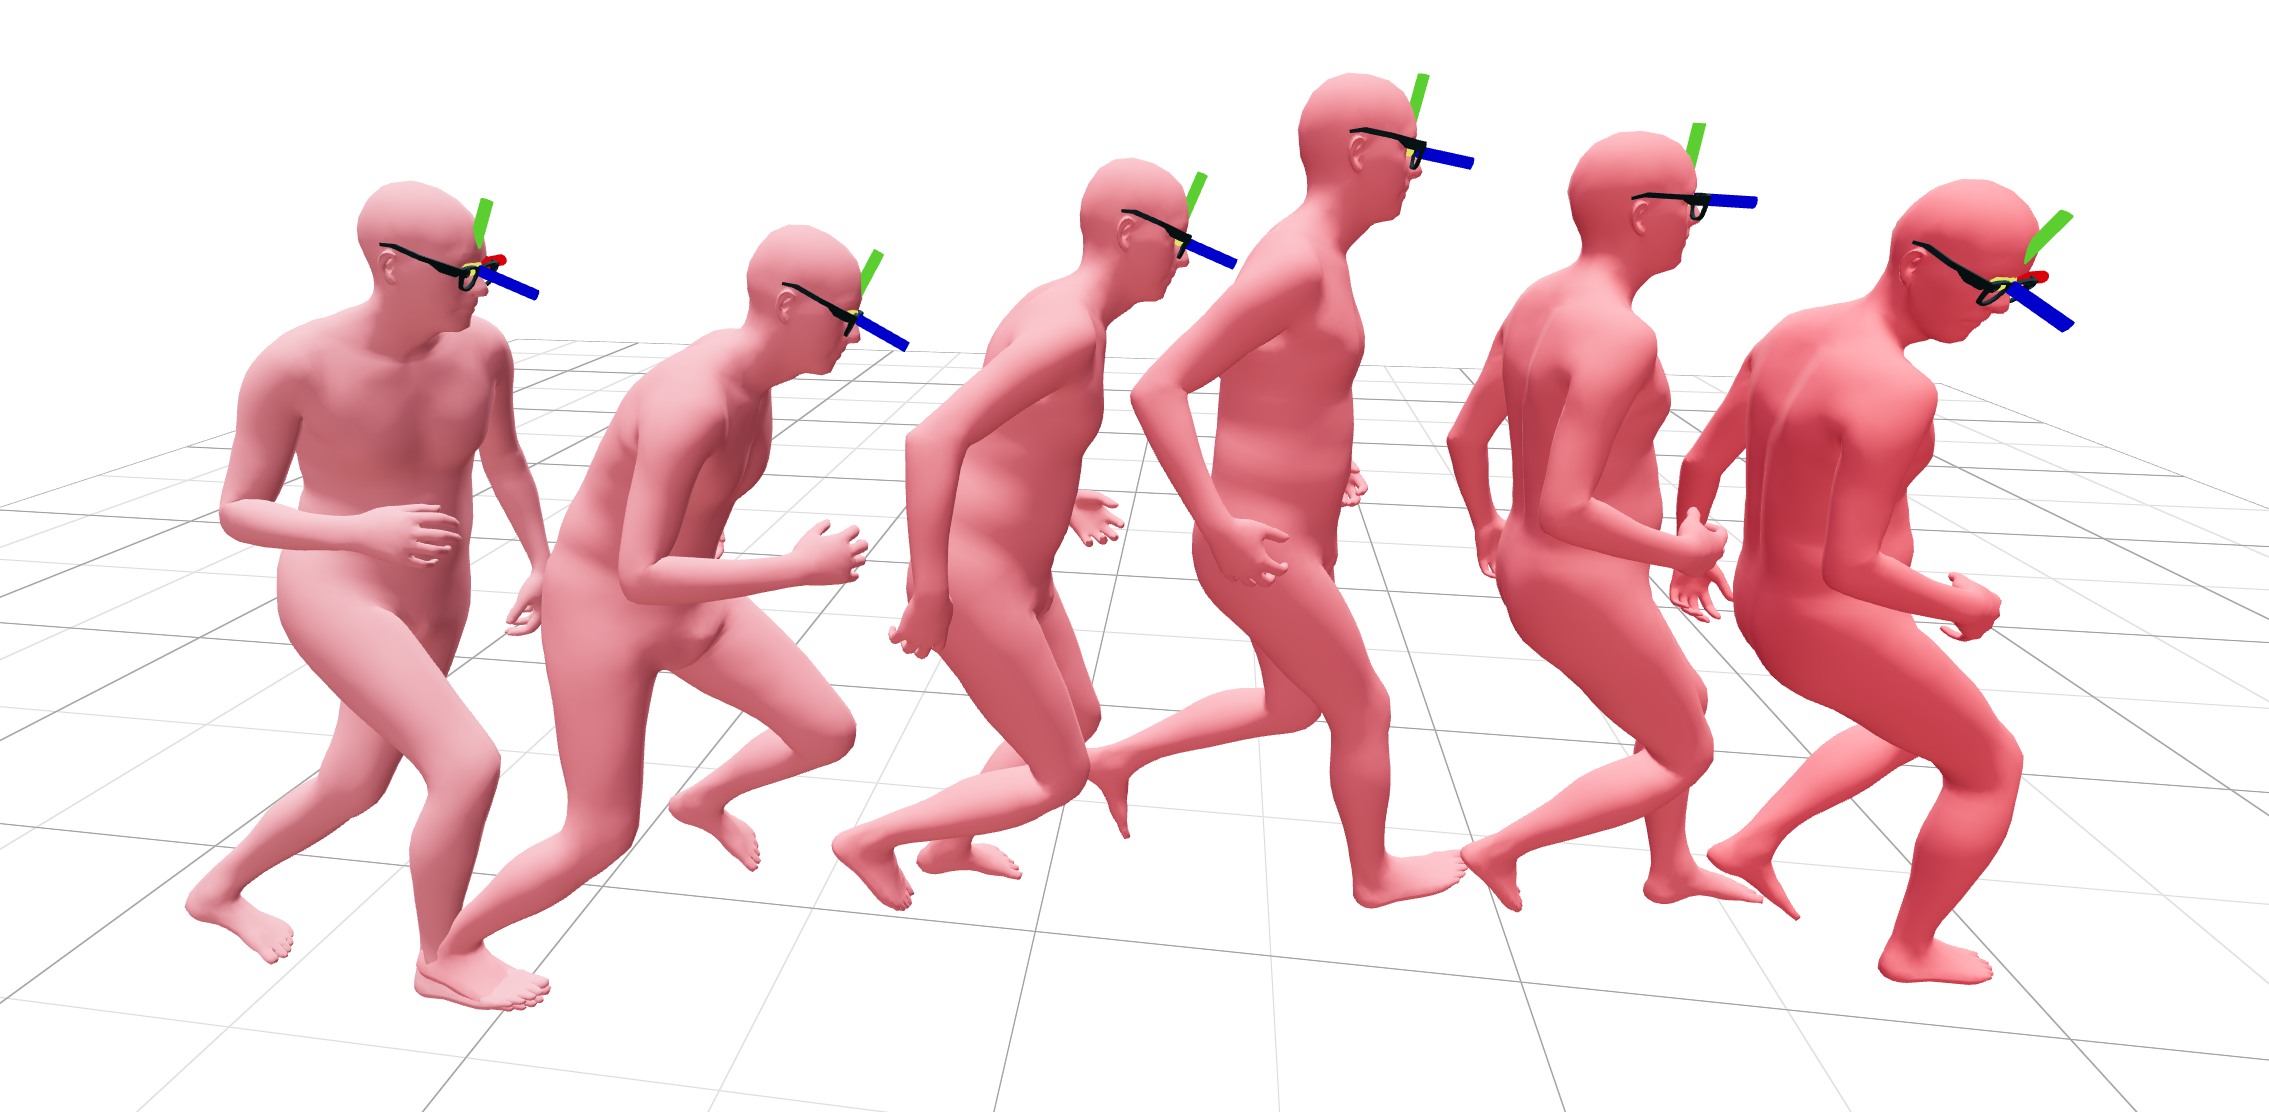
\includegraphics[width=\linewidth]{\toplevelprefix/chapters/chapter6/figs/qual0_gt.png}
  \caption{\centering 基准真值}
\end{subfigure}
\hfill
\begin{subfigure}{0.45\textwidth}
  \centering
  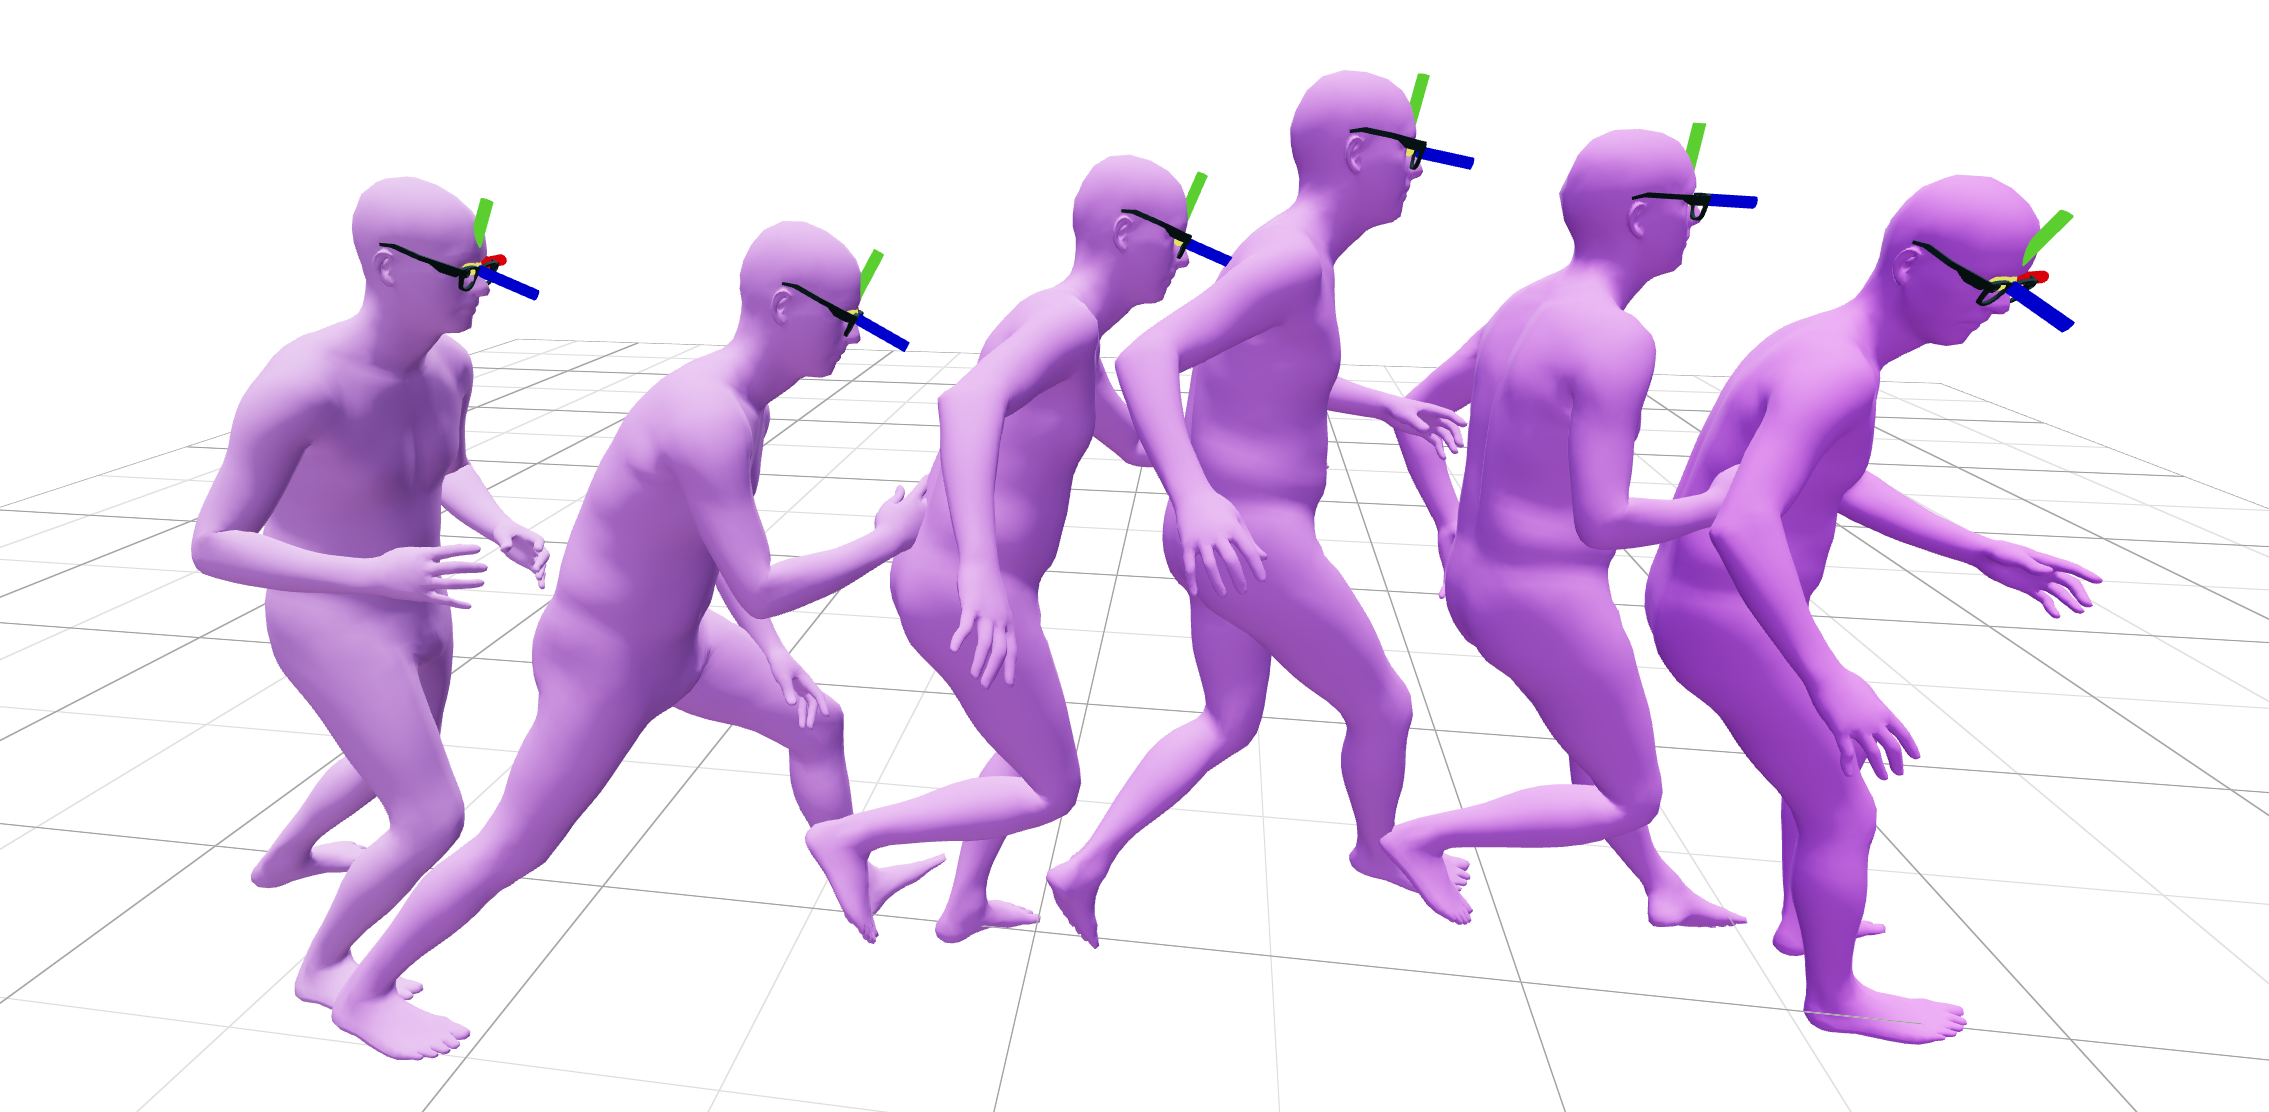
\includegraphics[width=\linewidth]{\toplevelprefix/chapters/chapter6/figs/qual0_ours.png}
  \caption{EgoAllo}
\end{subfigure}

% Second row
\begin{subfigure}{0.45\textwidth}
  \centering
  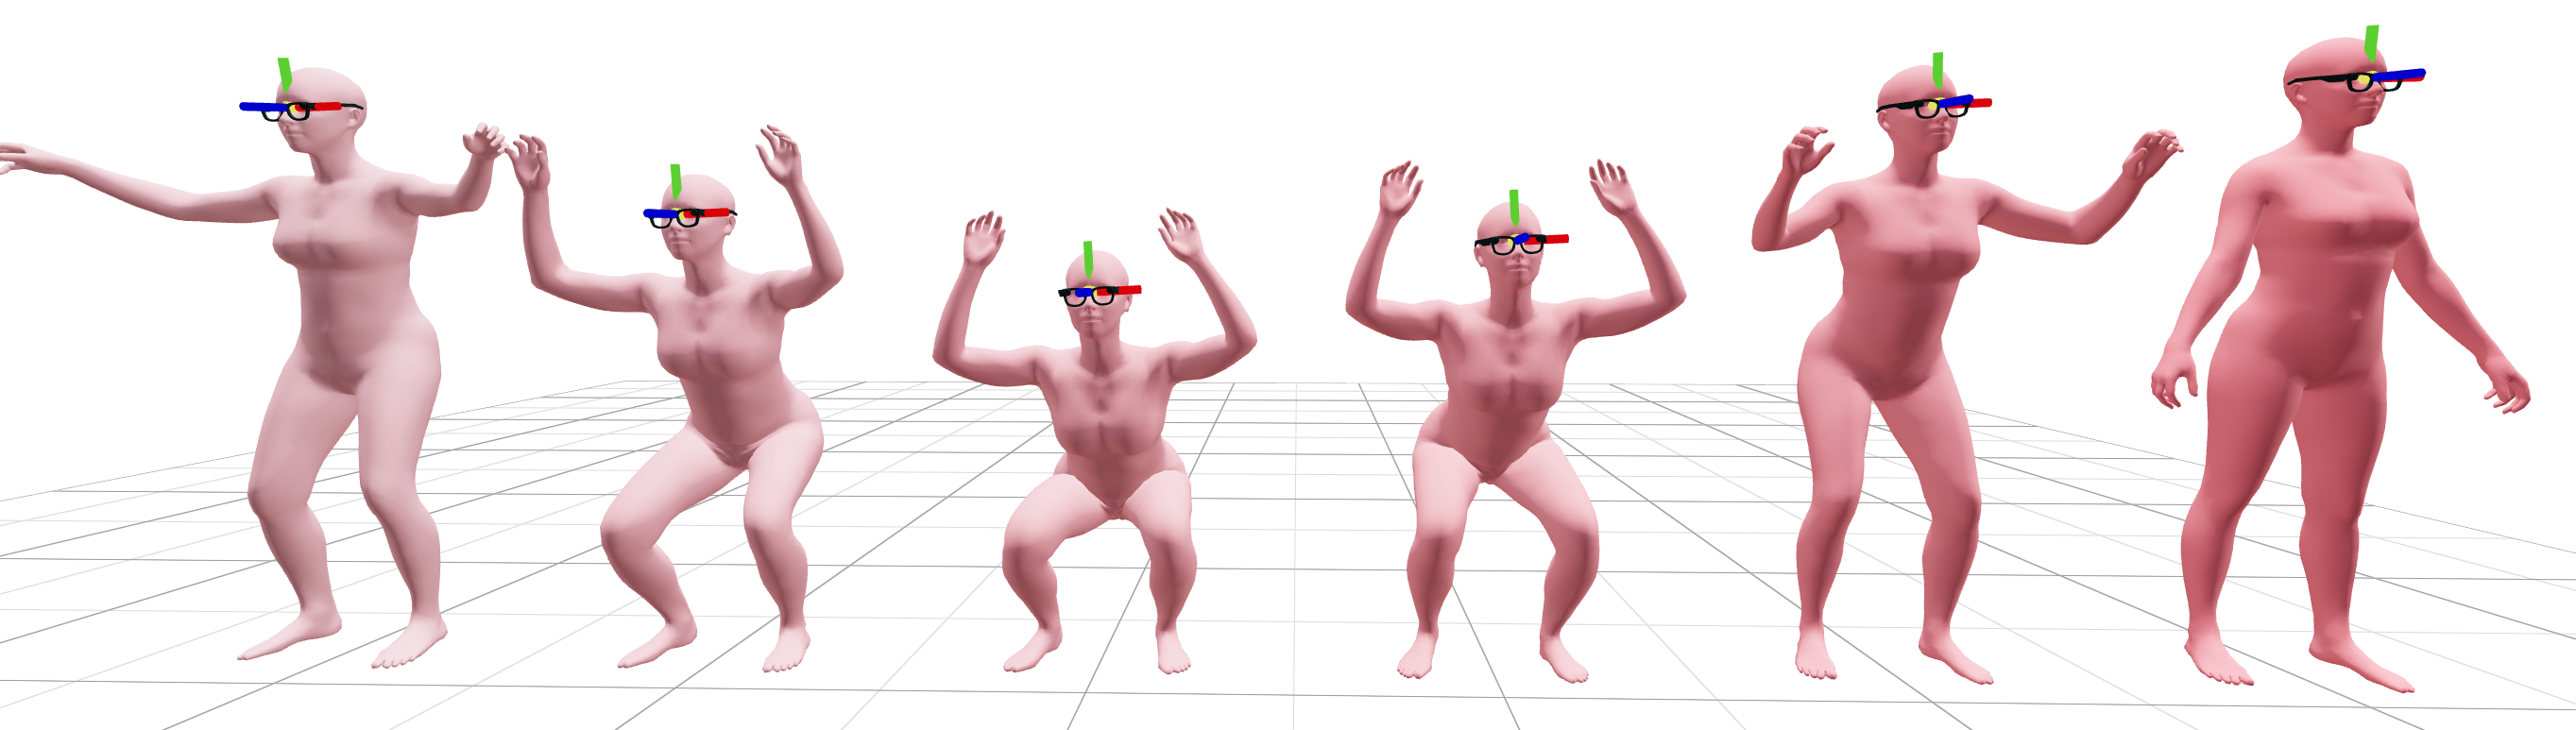
\includegraphics[width=\linewidth]{\toplevelprefix/chapters/chapter6/figs/qual1_gt.png}
  \caption{\centering 基准真值}
\end{subfigure}
\hfill
\begin{subfigure}{0.45\textwidth}
  \centering
  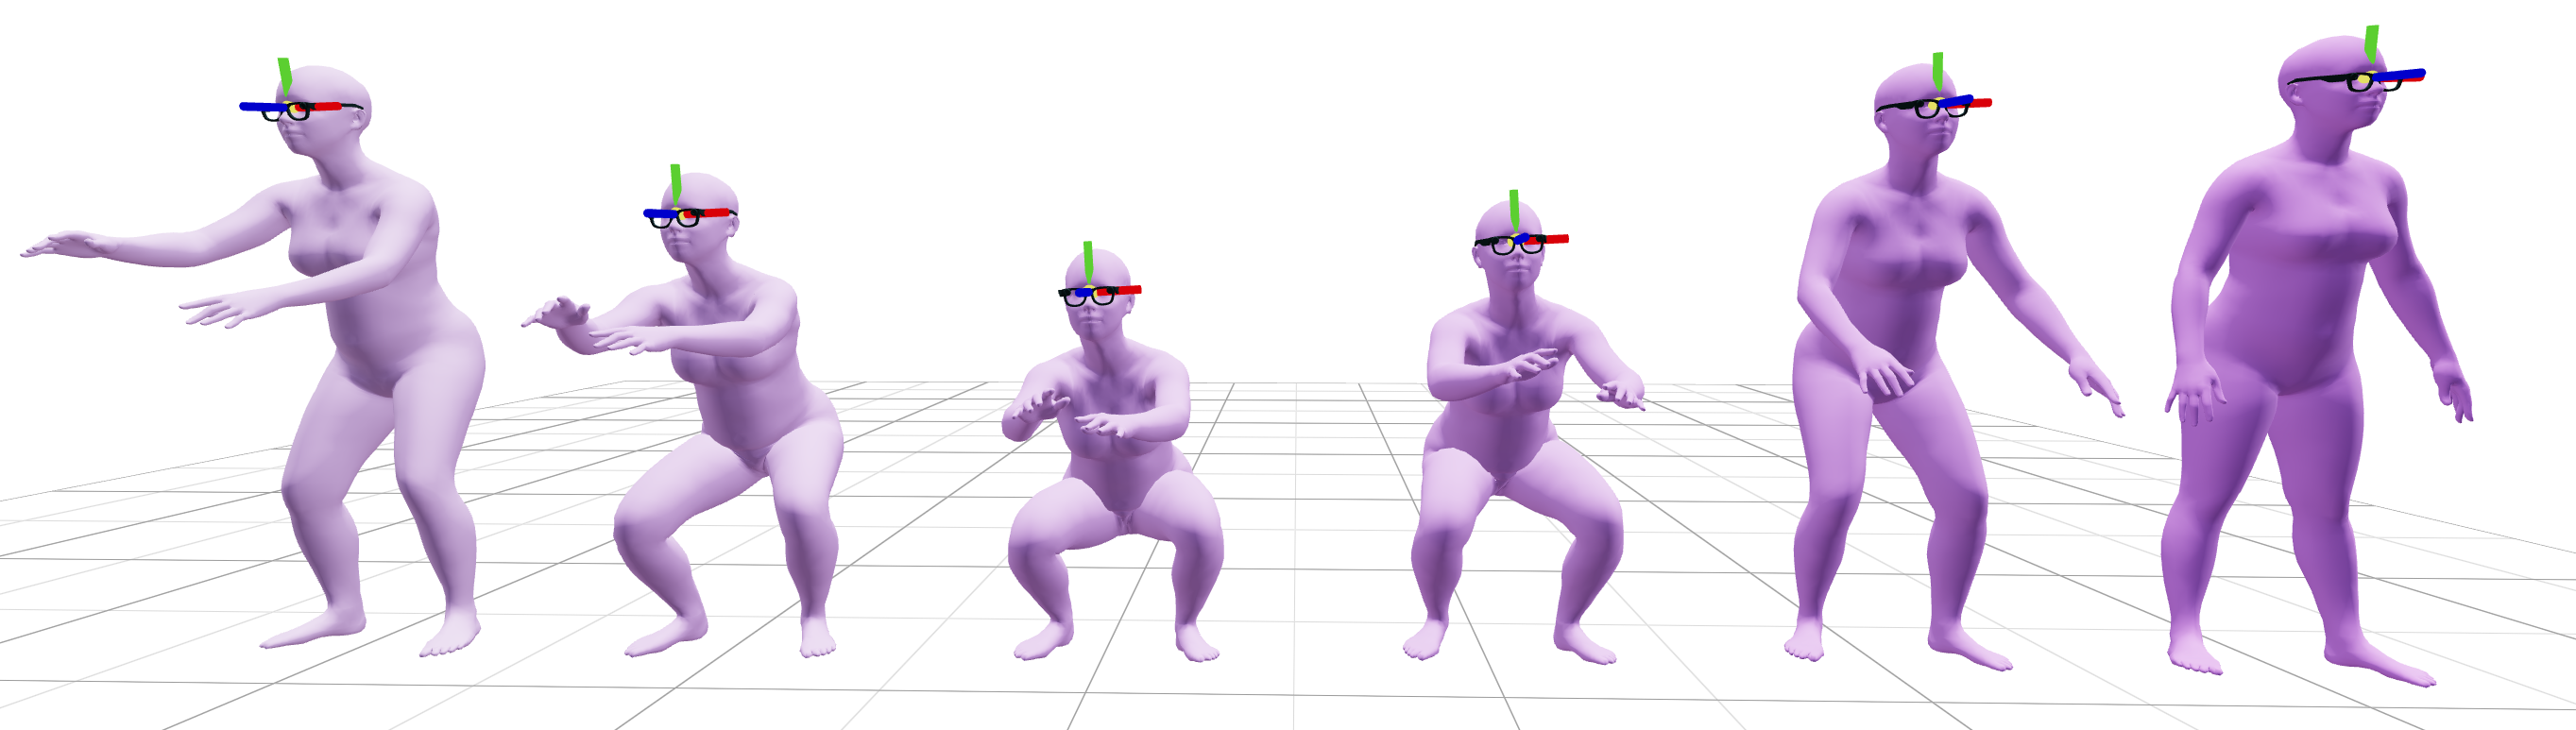
\includegraphics[width=\linewidth]{\toplevelprefix/chapters/chapter6/figs/qual1_ours.png}
  \caption{EgoAllo}
\end{subfigure}

\caption{
\textbf{一个跑步(上)和一个下蹲(下)序列的第一人称人体运动估计。}
基准真值运动与EgoAllo的一个输出进行比较,该输出与给定的头部姿态序列一致。
% 眼镜CAD模型被放置在条件变换$\textbf{T}_{\text{world},\text{cpf}}$处。
% 我们将输入条件姿态可视化为一个眼镜模型和坐标系。
}
\label{fig:comparison}
\end{figure}

严格来说,EgoAllo \cite{yi2024egoallo}中提出的解决方案并未使用上面介绍的技术来强制执行测量匹配。相反,它启发式地利用Transformer架构中的交叉注意力机制来强制施加条件。正如我们将在\Cref{sub:text-cond}中针对成对数据设定更精确地描述的那样,有理由相信交叉注意力机制在某种程度上近似地实现了后验去噪的条件采样。我们相信,如果这里介绍的更具原则性的技术得到妥善实施,可以带来更好的方法,进一步改善身体姿态和手势的估计。

\section{基于成对数据和测量的条件推断}
在许多实际应用中,我们既不知道我们所关心的数据 $\x$ 的分布,也不知道数据与某些观测到的属性 $\y$ 之间的显式关系。我们只有一个(大量的)配对样本集 $(\X, \Y) = \{ (\x_1, \y_1), \ldots, (\x_N, \y_N) \}$,我们需要从中推断数据分布以及一个建模它们之间关系的映射:
\begin{equation}
  h: \x \mapsto \y.
\end{equation}

图像分类问题可视作此类问题的一个实例。在某种意义上,分类问题是为自然图像学习一个(极度有损的)压缩编码器。也就是说,给定一个图像 $\x$ 的随机样本,我们希望预测其类别标签 $\y$,该标签能最好地关联 $\x$ 中的内容。我们知道,与像素空间的维度相比,物体在自然图像中的分布是低维的。从前面的章节中我们已经学到,原则上,只要有足够的样本,我们就可以通过学习一个压缩编码,为 $\x$ 学到一个结构化的低维表示 $\z$:
\begin{equation}
    f: \x \mapsto \z. 
\end{equation}
表示 $\z$ 也可以被看作是为 $\x$ 学习到的一个(有损但结构化的)编码。可以合理地假设,如果类别分配 $\y$ 确实依赖于 $\x$ 的低维结构,并且学习到的编码 $\z$ 确实反映了这种结构,那么 $\y$ 和 $\z$ 就可以变得高度相关,因此它们的联合分布 $p(\z, \y)$ 应该维度极低。因此,我们可以将这两个期望的编码 $\y$ 和 $\z$ 结合在一起,尝试学习一个组合编码器:
\begin{equation}
    f: \x \mapsto (\z, \y) 
\end{equation}
其中 $(\z, \y)$ 的联合分布是维度非常低的。

根据我们在前几章的学习,映射 $f$ 通常是作为同一空间中一系列压缩或去噪算子来学习的。因此,为了利用这类算子,我们可以引入一个辅助向量 $\vw$,它可以被看作是类别标签 $\y$ 的一个初始随机猜测。这样,我们就可以在一个共同的空间内学习一个压缩或去噪映射:
\begin{equation}\label{eq:classifier-with-class-token}
    f: (\x, \vw) \mapsto (\z, \y)
\end{equation}
事实上,在为分类任务训练 Transformer(例如在 ViT 中)时引入一个辅助“类别令牌”的普遍做法,可以被看作是通过压缩给定(带噪)样本 $(\x, \vw)$ 的(编码率)来学习这样一个表示。如果数据 $\x$ 的分布已经是(低维)高斯分布的混合,\cite{wright2008classification} 的工作已经表明,通过直接最小化与给定样本相关的{\em(有损)编码长度},可以有效地完成分类。


\subsection{类别条件的图像生成}\label{sub:cfg} 
虽然一个学习到的分类器允许我们将给定的图像 $\x$ 分类到其对应的类别,但我们通常也希望生成一个给定类别的图像,这需要对学习到的自然图像分布进行采样。在某种程度上,这可以被看作是图像分类的“逆”问题。设 $p_{\x}$ 表示自然图像的分布,例如通过一个扩散-去噪过程来建模。给定一个类别标签随机变量 $y \in [K]$,其实际值为 $\nu$,比如说“苹果”,我们希望对条件分布 $p_{\x \mid y}(\,\cdot\, \mid \nu)$ 进行采样,以生成一张苹果的图像:
\begin{equation}
  %g: \vnu \mapsto \hat{\x}, \quad 
  \hat{\x} \sim p_{\x\mid \y}(\,\cdot\, \mid \vnu).
\end{equation}
我们称之为{\em 类别条件的图像生成}。

在 \Cref{sec:conditioned-decoding} 中,我们已经看到了如何使用去噪-扩散范式,在给定\textit{基于模型的}测量 $\vy = h(\vx) + \vw$(\Cref{eq:measurement-matching-observation})的情况下,从后验 $p_{\vx \mid \vy}$ 进行条件采样,最终得到了 DPS 算法 \eqref{alg:iterative_denoising_conditional_DPS}。这是一个强大的框架,但它不适用于这里的类别(或文本)条件的图像生成问题,因为观测/属性 $y$ 的显式生成模型 $h$ 由于解析建模的棘手性而无法获得。在本节中,我们将介绍将条件采样扩展到此设定的技术。


因此,我们现在只假设我们能够从 $(\vx, y)$ 的联合分布中获取样本:
\begin{equation}
  (\vx, y) \sim p_{\vx, y}.
\end{equation}
% Our goal remains to produce conditional samples $\hat{\vx}$ from the posterior,
% given realizations $\vnu$ of $\vy$:
% \begin{equation}
%   \hat{\vx} \sim p_{\vx \mid \vy}(\spcdot \mid \vnu).
% \end{equation}
与前一节一样,我们定义 $\vx_t = \alpha_t \vx + \sigma_t \vg$,其中 $\vg \sim \cN(\Zero, \vI)$ 且独立于 $(\vx, \vy)$,这与 \Cref{ch:compression} 中的 \Cref{eq:gen_additive_gaussian_noise_model} 一致,并且我们将反复使用符号 $\vxi$ 来表示 $\vx$ 和 $\vx_t$ 的实现。

为了继续,我们注意到,我们对在测量 $\vy = h(\vx) + \vw$ 下的条件采样的推导,仅在进行 DPS 近似 \eqref{eq:conditional-posterior-measurementmatching-gaussian-case-dps-approx} 时明确使用了前向模型 $h$。特别地,条件后验去噪器分解 \eqref{eq:posterior-sampling-denoiser-decomposition} \textit{在配对数据设定下仍然成立},这是由于贝叶斯法则以及在给定 $\vx$ 的情况下 $\vy$ 和 $\vx_t$ 的条件独立性(回想 \Cref{fig:posterior-sampling-cds})。因此,在配-对数据设定下我们仍然可以写出
\begin{equation}\label{eq:conditional-denoising-mmse-denoiser-paired-data}
  \bE[ \vx \mid \vx_t=\vxi, y=\nu]
  =
  \bE[\vx \mid \vx_t=\vxi] 
  + \frac{\sigma_t^2}{\alpha_t} 
  \nabla_{\vxi}\log p_{y \mid \vx_t}(\nu\mid \vxi).
\end{equation}
一个自然的想法是直接使用一个带有参数 $\theta_{\mathrm{c}}$ 的深度网络 $f_{\theta_{\mathrm{c}}}$ 来实现 \eqref{eq:conditional-denoising-mmse-denoiser-paired-data} 中的似然校正项,如 \Cref{eq:classifier-with-class-token} 中所示:
% which maps noisy samples
% $\vx_t$ (and, as is common in practice, the time $t$ in the noising process) to
% a probability distribution over class labels $\vy$:
\begin{equation}
  f_{\theta_{\mathrm{c}}} : (t, \vx_t) \mapsto \softmax(\vW_{\mathrm{head}}
  \vz(t, \vx_t)).
\end{equation}
这个表达式将带噪输入 $\vx_t$ 的最终表示 $\vz(t, \vx_t)$(也依赖于 $\theta_{\mathrm{c}}$)与一个分类头 $\vW_{\mathrm{head}} \in \bR^{K \times d}$ 结合起来,该分类头将表示映射到 $K$ 个可能类别上的概率分布。
在实践中,通常也会将加噪过程中的时间 $t$ 作为输入。
因此,通过适当的训练,它提供了对数似然 $\log p_{y \mid \vx_t}$ 的一个近似,并且对 $\log f_{\theta_{\mathrm{c}}}$ 关于其输入 $\vx_t$ 求导,可以得到 \Cref{eq:conditional-denoising-mmse-denoiser-paired-data} 中第二项的近似:
\begin{equation}\label{eq:conditional-denoising-mmse-denoiser-paired-data-approx}
  % \bE[ \vx \mid \vx_t=\vxi, \vy=\vnu]
  \bar{\vx}_{\theta}^{\mathrm{naive}}(t, \vx_t, y)
  =
  % \bE[\vx \mid \vx_t=\vxi] 
  \bar{\vx}_{\theta_{\mathrm{d}}}(t, \vx_t)
  + \frac{\sigma_t^2}{\alpha_t}
  \nabla_{\vx_t}
  \ip*{
    \log f_{\theta_{\mathrm{c}}}(t, \vx_t)
  }{
    \ve_{y}
  }
\end{equation}
这里,像往常一样,我们通过一个学习到的、带有参数 $\theta_{\mathrm{d}}$ 的无条件去噪器来近似 \Cref{eq:conditional-denoising-mmse-denoiser-paired-data} 中的第一项,并且我们用 $\ve_k$(对于 $k \in [K]$)表示 $\R^K$ 的第 $k$ 个标准基向量(即在第 $k$ 个位置为 1,其他位置为 0 的向量)。
读者应该注意到,条件去噪器 $\bar{\vx}_{\theta}$ 需要两次独立的训练过程,使用不同的损失函数:一次是针对分类器参数 $\theta_{\mathrm{c}}$ 的分类损失,\footnote{在 \Cref{ch:applications} 中,我们详细回顾了训练这样一个分类器的过程。} 另一次是针对去噪器参数 $\theta_{\mathrm{d}}$ 的去噪损失。这种条件采样方法在扩散模型的早期开创性工作中已经被认识到并加以利用,特别是 \citet{Sohl-Dickstein2015} 和 \citet{song2020score} 的工作。
% To use \eqref{eq:conditional-denoising-mmse-denoiser-paired-data-approx} at
% sampling time, it suffices to substitute
% \eqref{eq:conditional-denoising-mmse-denoiser-paired-data-approx} for the 

% the network maps noisy data samples $\vx_t$ to a probability distribution over
% measurements $\vy$, then one evaluates its gradient with respect to $\vx_t$
% using backpropagation to compute the correction term in
% \Cref{eq:conditional-denoising-mmse-denoiser-paired-data}.
% Such an approach was already recognized and exploited to perform conditional
% sampling in pioneering early works on diffusion models, notably those by
% \citet{Sohl-Dickstein2015} and by \citet{song2020score}. For example, in the
% setting where $\vy$ corresponds to a class label taking values in the index set
% $\set{1, \dots, K}$, a deep network mapping noisy
% inputs and their corresponding noise levels $(\vx_t, t) \in \bR^{D} \times
% \bR$ to a probability distribution over labels $y \in \set{1, \dots, K}$ can be
% trained via the standard cross entropy training with a labeled dataset by adding
% independent noise to the training images.

然而,这种直接的方法有两个关键的缺点(这也是我们称之为“朴素”的原因)。第一个是,根据经验,这样一个训练好的深度网络分类器通常不能提供足够强的指导信号(在 \Cref{eq:conditional-denoising-mmse-denoiser-paired-data} 中),以确保生成的样本能反映条件信息 $y$。这一点首先由 \citet{Dhariwal2021-hg} 强调,他们指出,在类别条件的 ImageNet 生成任务中,学习到的深度网络分类器对条件类别 $y$ 的概率输出常常在 $0.5$ 左右——虽然足以成为主导类别,但不足以提供强大的指导信号——并且经检查,生成的图像与条件类别 $y$ 不一致。\citet{Dhariwal2021-hg} 提议通过在朴素条件去噪器 \eqref{eq:conditional-denoising-mmse-denoiser-paired-data-approx} 的定义中引入一个“逆温度”超参数 $\gamma > 0$ 来启发式地解决这个问题,并将得到的条件去噪器称为融入了“分类器指导”(CG):
\begin{equation}\label{eq:conditional-denoising-mmse-denoiser-paired-data-approx-cg}
  \bar{\vx}_{\theta}^{\mathrm{CG}}(t, \vx_t, y)
  =
  \bar{\vx}_{\theta_{\mathrm{d}}}(t, \vx_t)
  + \gamma\frac{\sigma_t^2}{\alpha_t}
  \nabla_{\vx_t}
  \ip*{
    \log f_{\theta_{\mathrm{c}}}(t, \vx_t)
  }{
    \ve_{y}
  }
\end{equation}
其中 $\gamma = 1$ 的情况与 \eqref{eq:conditional-denoising-mmse-denoiser-paired-data-approx} 一致。
\citet{Dhariwal2021-hg} 发现,在经验上,设置 $\gamma > 1$ 的表现最好。
对此一个可能的解释如下:注意,在\textit{真实}似然项 \Cref{eq:conditional-denoising-mmse-denoiser-paired-data} 的背景下,乘以 $\gamma$ 等价于
\begin{align}
  \gamma\frac{\sigma_t^2}{\alpha_t} \nabla_{\vxi}\log p_{\vy \mid \vx_t}(\vnu\mid
  \vxi)
  &=
  \frac{\sigma_t^2}{\alpha_t} \nabla_{\vxi}\log \left(
  p_{\vy \mid \vx_t}(\vnu\mid \vxi)^\gamma
  \right), %\\
  % &=
  % \frac{\sigma_t^2}{\alpha_t} \nabla_{\vxi}\log \left(
  % \frac{
  %   p_{\vy \mid \vx_t}(\vnu\mid \vxi)^w
  % }{
  %   \int p_{\vy \mid \vx_t}(\vnu'\mid \vxi)^w \odif \vnu'
  % }
  % \right)
\end{align}
这自然地引出了参数 $\gamma$ 是对似然 $p_{\vy \mid \vx_t}$ 进行(逆)\textit{温度缩放}的解释,如果我们考虑重归一化分布 $ { p_{\vy \mid \vx_t}(\vnu\mid \vxi)^\gamma } / { \int p_{\vy \mid \vx_t}(\vnu'\mid \vxi)^\gamma \odif \vnu' } $,这个解释是精确的。
然而,请注意,在 \Cref{eq:conditional-denoising-mmse-denoiser-paired-data} 的背景下,这\textit{不是}一个严格的解释,因为梯度是关于 $\vxi$ 计算的,而温度缩放分布中的归一化常数通常是 $\vxi$ 的函数。
相反,参数 $\gamma$ 应该被简单地理解为放大了深度网络分类器输出概率 $f_{\theta_{\mathrm{c}}}(t, \vx_t)$ 的大值\textit{相对于}小值,这在深度网络 $f$ 将其分配为 $K$ 个类别中最大概率的情况下,有效地放大了提供的指导信号。
% We will return to this point \sdb{in a subsequent example}.
% Regardless, choosing $w > 1$ has the effect of exaggerating large values of the
% likelihood $p_{\vy \mid \vx_t}$ relative to smaller ones, which amplifies the
% guidance signal provided, leading to dramatic improvements in generation quality
% and faithfulness to the conditioning signal in practice.

% \begin{example}[Classification] One may view the problem of
% classification as a special case for completing or predicting
% missing parts of a random vector. For classification, given a
% sample vector $\x$, we would like to predict its class label $\y$.
% If we stack the two together as one joint vector:
% \begin{equation}
%   \vw = (\x, \y),
% \end{equation}
% one may view the problem of predicting the class label $\y$ as a
% problem of completing $\vw$ by observing only the $\x$ part. This
% is usually done by estimating and transforming the joint
% distribution of $\vw$ that minimizes the entropy (or coding
% rate) of the resulting representation of the empirical distribution
% of $\vx$.\footnote{A set of samples for $\x$ and their associated
% class labels $\y$} In fact, the common practice of introducing an
% auxiliary ``class token'' in the training of a Transformer for
% classification tasks can be viewed as learning such a
% representation by compressing (the coding rate of) given samples of
% $\vw$. If the distribution of the data $\x$ is already a
% mixture of (low-dimensional) Gaussians, the work
% \cite{wright2008classification} showed that classification can be
% done effectively by directly minimizing {\em the (lossy) coding
% length} associated with the given samples.
% \end{example}

然而,分类器指导并没有解决朴素方法的第二个关键缺点:除了无条件去噪器 $\bar{\vx}_{\theta_{\mathrm{d}}}$ 之外,还必须训练一个辅助分类器 $f_{\theta_{\mathrm{c}}}$,这既繁琐又浪费,因为无法直接调整一个预训练的分类器来使其在带噪输入 $\vx_t$ 上表现良好,并融入其他经验驱动的架构修改。
特别地,\citet{Dhariwal2021-hg} 发现,有必要明确设计实现分类器的深度网络架构,以匹配去噪器的架构。
此外,从纯粹的实践角度——试图从最终的采样器中获得最佳性能——表现最佳的基于分类器指导的采样配置甚至进一步偏离了我们上面介绍的理想化和概念上合理的框架。
为了获得最佳性能,\citet{Dhariwal2021-hg} 发现有必要将类别标签 $y$ 作为额外输入提供给去噪器 $\bar{\vx}_{\theta_{\mathrm{d}}}$。因此,由 \citet{Dhariwal2021-hg} 如我们上面从条件后验去噪器分解 \eqref{eq:conditional-denoising-mmse-denoiser-paired-data} 推导出的理想化分类器指导去噪器 \eqref{eq:conditional-denoising-mmse-denoiser-paired-data-approx-cg},并不能完全反映实践中表现最佳的去噪器——这样的去噪器实际上是将一个给定 $y$ 的\textit{条件}去噪器与来自辅助分类器的额外指导信号相结合!

这种由经验驱动的状况,导致 \citet{Ho2022-ry} 在后续工作中提出了一种更具经验实用性的方法,称为无分类器指导(CFG)。他们没有将条件去噪器 \eqref{eq:conditional-denoising-mmse-denoiser-paired-data} 表示为无条件去噪器与对数似然校正项的加权和(可能像在分类器指导中那样修改权重),而是接受了训练一个给定 $y$ 的条件去噪器的明显必要性,正如 \citet{Dhariwal2021-hg} 的实验结果所证明的那样,并用这个条件去噪器与一个给定 $\vx_t$ 的\textit{无条件}去噪器的正确加权和来替换对数似然梯度项。\footnote{话虽如此,\textcite{Ho2022-ry} 实际上提出了使用与我们在此处呈现的不同的加权方式,这是基于 \textcite{Dhariwal2021-hg} 启发式地将 \eqref{eq:conditional-denoising-mmse-denoiser-paired-data} 中的无条件去噪器替换为条件去噪器的事实。实际上,我们推导并在此处呈现的加权方式反映了现代实践,特别是在最先进的扩散模型如 Stable Diffusion 3.5 \cite{DBLP:conf/icml/EsserKBEMSLLSBP24} 中使用。} 为了看清这种结构是如何产生的,我们从 \eqref{eq:conditional-denoising-mmse-denoiser-paired-data-approx-cg} 中定义的分类器指导去噪器 $\bar{\vx}_{\theta}^{\mathrm{CG}}$ 的一个“理想化”版本开始,其中去噪器 $\bar{\vx}_{\theta_{\mathrm{d}}}$ 和分类器 $f_{\theta_{\mathrm{c}}}$ 通过 \eqref{eq:conditional-denoising-mmse-denoiser-paired-data} 完美地逼近了它们的目标:
\begin{equation}\label{eq:conditional-denoising-mmse-denoiser-paired-data-exact-cg}
  \bar{\vx}_{\theta}^{\mathrm{CG,\,ideal}}(t, \vxi, \nu)
  =
  \bE[\vx \mid \vx_t=\vxi]
  + \gamma\frac{\sigma_t^2}{\alpha_t}
  \nabla_{\vxi}\log p_{y \mid \vx_t}(\nu\mid \vxi).
\end{equation}
然后我们使用贝叶斯法则,其形式为
\begin{equation}
  \log p_{y \mid \vx_t}
  =
  \log p_{\vx_t \mid y} + \log p_{y} - \log p_{\vx_t},
\end{equation}
并结合特威迪公式(\Cref{thm:tweedie},按 \Cref{eq:gen_tweedie} 修改)在得分函数和去噪器之间进行转换,得到
\begin{align*}
  \bar{\vx}_{\theta}^{\mathrm{CG,\,ideal}}(t, \vxi, \nu)
  &=
  % \bE[\vx \mid \vx_t=\vxi]
  % + \gamma\frac{\sigma_t^2}{\alpha_t}
  % \nabla_{\vxi}\log p_{y \mid \vx_t}(\nu\mid \vxi).
  \frac{1}{\alpha_t} \vxi 
  + (1-\gamma) \frac{\sigma_t^2}{\alpha_t} 
  \nabla_{\vxi}\log p_{\vx_t}(\vxi)
  + \gamma \frac{\sigma_t^2}{\alpha_t} 
  \nabla_{\vxi}\log p_{\vx_t \mid y}(\vxi \mid \nu)
  \\
  &=
  (1 - \gamma) \bE[\vx \mid \vx_t=\vxi]
  +
  \gamma \bE[\vx \mid \vx_t=\vxi, y=\nu],
  \labelthis\label{eq:ideal-cfg-denoiser}
\end{align*}
在最后一行,我们应用了 \Cref{eq:conditional-denoising-conditioning-order-irrelevant}。
现在,\Cref{eq:ideal-cfg-denoiser} 提出了一个自然的近似策略:我们将一个学习到的、给定 $\vx_t$ 的无条件去噪器与一个学习到的、给定 $\vx_t$ 和 $y$ 的\textit{条件}去噪器相结合。

%\yima{Following the geometric interpretation of the conditional generation, how effective the above approaches are to utilize the conditional probability $p(y\mid \x)$ depends on whether the conditional probability is given in a form of an effective constraint on $\x$.}

然而,遵循 \textcite{Ho2022-ry} 和训练深度网络去噪器的普遍做法,标准做法是使用\textit{同一个}深度网络来表示条件和无条件去噪器,通过引入一个额外的标签,我们将其表示为 $\varnothing$,来表示“无条件”情况。
这导致了 CFG 去噪器的形式:
\begin{equation}\label{eq:conditional-denoising-mmse-denoiser-paired-data-approx-cfg}
  \bar{\vx}_{\theta}^{\mathrm{CFG}}(t, \vx_t, y)
  =
  (1 - \gamma) \bar{\vx}_{\theta}(t, \vx_t, \varnothing)
  +
  \gamma \bar{\vx}_{\theta}(t, \vx_t, y).
\end{equation}
为了训练一个用于无分类器指导采样的去噪器 $\bar{\vx}_{\theta}(t, \vx_t, y^+)$,其中 $y^+ \in \set{1, \dots, K, \varnothing}$,我们的做法与 \Cref{alg:learning_denoiser} 中的无条件训练过程几乎相同,但有两处修改:
\begin{enumerate}
  \item 当我们从数据集中采样时,我们采样一个对 $(\vx, y)$ 而不仅仅是一个样本 $\vx$。
  \item 每当我们从数据集中采样一个对时,我们通过以下方式采样增强标签 $y^+$:
    \begin{equation}
      y^+ = \begin{cases}
        \varnothing & \text{以概率 } p_{\mathrm{uncond}}; \\
        y & \text{其他情况}.
      \end{cases}
    \end{equation}
    这里,$p_{\mathrm{uncond}} \in [0, 1]$ 是一个新的超参数。
    这可以被看作是 dropout \cite{srivastava2014dropout} 的一种形式。
\end{enumerate}
通过这种方式,我们训练了一个适用于无分类器指导采样的条件去噪器。我们在 \Cref{alg:iterative_denoising_conditional_CFG} 中总结了使用无分类器指导进行类别条件采样的整个采样过程。

% \sdb{I think it makes sense just to present the algorithm box for CFG.}
% \begin{algorithm}
%   \caption{Conditional sampling with classification data, with an unconditional
%   denoiser and guidance.}
% 	\label{alg:iterative_denoising_conditional_CG}
% 	\begin{algorithmic}[1]
% 		\Require{An ordered list of timesteps \(0 \leq t_{0} < \cdots < t_{L} \leq T\) to use for sampling.}
%     \Require{An unconditional denoiser \(\bar{\vx}_{\theta} \colon
%     \{t_{\ell}\}_{\ell = 1}^{L} \times \R^{D} \to \R^{D}\) for $p_{\vx}$.}
%     \Require{Class label $\nu \in \set{1, \dots, K}$ to condition on.}
%     \Require{Forward model $h : \bR^D \to \bR^d$ and measurement noise variance
%     $\sigma^2 > 0$.}
% 		\Require{Scale and noise level functions \(\alpha, \sigma \colon \{t_{\ell}\}_{\ell = 0}^{L} \to \R_{\geq 0}\).}
%     \Ensure{A sample \(\hat{\vx}\), approximately from \(p_{y \mid \vx}(\nu \mid
%     \,\cdot\,)\).}
%     \Function{DDIMSamplerConditionalDPS}{$\bar{\vx}_{\theta}, \nu, \sigma^2,
%     (t_{\ell})_{\ell = 0}^{L}$}
% 		\State{Initialize \(\hat{\vx}_{t_{L}} \sim\) approximate distribution of \(\vx_{t_{L}}\)} \Comment{VP \(\implies \dNorm(\vzero, \vI)\), VE \(\implies \dNorm(\vzero, t_{L}^{2}\vI)\).}
% 		\For{\(\ell = L, L - 1, \dots, 1\)}
% 		% \State{Compute
% 		% 	\begin{equation*}
%   %       \nabla_{\vxi}\left[ -\frac{1}{2\sigma^2} \norm*{h(
%   %       \bar{\vx}_{\theta}(t_{\ell}, \vxi)
%   %       ) - \vnu}_2^2 \right]\biggl|_{\vxi = \hat{\vx}_{t_{\ell}}}\biggr.
% 		% 	\end{equation*}
% 		% }
% 		\State{Compute
% 			\begin{equation*}
% 				\hat{\vx}_{t_{\ell - 1}} \doteq \frac{\sigma_{t_{\ell
%         - 1}}}{\sigma_{t_{\ell}}}\hat{\vx}_{t_{\ell}} + \bp{\alpha_{t_{\ell
%         - 1}} - \frac{\sigma_{t_{\ell
%         - 1}}}{\sigma_{t_{\ell}}}\alpha_{t_{\ell}}}\left(
%         \bar{\vx}_{\theta}(t_{\ell}, \hat{\vx}_{t_{\ell}})
%         - \frac{\sigma_{t_{\ell}}^2}{2\alpha_{t_\ell}\sigma^2}
%         \nabla_{\vxi}\left[ \norm*{h( \bar{\vx}_{\theta}(t_{\ell}, \vxi)
%         ) - \vnu}_2^2 \right]\biggl|_{\vxi = \hat{\vx}_{t_{\ell}}}\biggr.
%         \right)
% 			\end{equation*}
% 		}
% 		\EndFor
% 		\State{\Return{\(\hat{\vx}_{t_{0}}\)}}
% 		\EndFunction
% 	\end{algorithmic}
% \end{algorithm}

\begin{algorithm}
  \caption{使用类别条件去噪器,对分类数据进行条件采样。}
	\label{alg:iterative_denoising_conditional_CFG}
	\begin{algorithmic}[1]
		\Require{用于采样的一系列有序时间步 \(0 \leq t_{0} < \cdots < t_{L} \leq T\)。}
    \Require{要作为条件的类别标签 $\nu \in \set{1, \dots, K}$。}
    \Require{一个用于 $p_{\vx \mid y}$ 和 $p_{\vx}$ 的去噪器 \(\bar{\vx}_{\theta} \colon \{t_{\ell}\}_{\ell = 1}^{L} \times \R^{D} \times \set{1, \dots, K, \varnothing} \to \R^{D}\)(对于 $p_{\vx}$ 输入 $\varnothing$)。}
		\Require{尺度和噪声水平函数 \(\alpha, \sigma \colon \{t_{\ell}\}_{\ell = 0}^{L} \to \R_{\geq 0}\)。}
    \Require{指导强度 $\gamma \geq 0$(为获得更好性能,推荐 $\gamma > 1$)。}
    \Ensure{一个样本 \(\hat{\vx}\),近似来自 \(p_{\vx \mid y}(\,\cdot\, \mid \nu)\)。}
    \Function{DDIMSamplerConditionalCFG}{$\bar{\vx}_{\theta}, \nu, \gamma, (t_{\ell})_{\ell = 0}^{L}$}
		\State{初始化 \(\hat{\vx}_{t_{L}} \sim\) \(\vx_{t_{L}}\) 的近似分布} \Comment{VP \(\implies \dNorm(\vzero, \vI)\), VE \(\implies \dNorm(\vzero, t_{L}^{2}\vI)\)。}
		\For{\(\ell = L, L - 1, \dots, 1\)}
		% \State{Compute
		% 	\begin{equation*}
  %       \nabla_{\vxi}\left[ -\frac{1}{2\sigma^2} \norm*{h(
  %       \bar{\vx}_{\theta}(t_{\ell}, \vxi)
  %       ) - \vnu}_2^2 \right]\biggl|_{\vxi = \hat{\vx}_{t_{\ell}}}\biggr.
		% 	\end{equation*}
		% }
		\State{计算
			\begin{equation*}
				\hat{\vx}_{t_{\ell - 1}} \doteq \frac{\sigma_{t_{\ell
        - 1}}}{\sigma_{t_{\ell}}}\hat{\vx}_{t_{\ell}} + \bp{\alpha_{t_{\ell
        - 1}} - \frac{\sigma_{t_{\ell
        - 1}}}{\sigma_{t_{\ell}}}\alpha_{t_{\ell}}}\bigl(
        (1 - \gamma) \bar{\vx}_{\theta}(t_{\ell}, \hat{\vx}_{t_{\ell}}, \varnothing)
        + \gamma \bar{\vx}_{\theta}(t_{\ell}, \hat{\vx}_{t_{\ell}}, \nu)
        \bigr)
			\end{equation*}
		}
		\EndFor
		\State{\Return{\(\hat{\vx}_{t_{0}}\)}}
		\EndFunction
	\end{algorithmic}
\end{algorithm}

\textcite{Ho2022-ry} 报告了无分类器指导在类别条件图像生成方面的强大经验性能,并且它已成为最大规模的实用扩散模型(如 Stable Diffusion \cite{rombach2022high} 及其衍生品)的支柱。
同时,它的推导过程相当不透明且受经验驱动,对其强大性能背后的机制提供的洞见甚少。
一些理论工作研究了这一点,为整个 CFG 方法的某些部分提供了解释 \cite{Bradley2024-jg,Li2025-li,Wu2024-js}——其本身涵盖了去噪器的参数化和训练,以及指导强度的配置和采样时的性能。
下面,我们将在一个简化的设置中给出一个解释,即高斯混合模型数据分布和去噪器,这将展示 %
% an interesting connection to the rate reduction objective studied in
% chapters \Cref{ch:compression,ch:unrolling}, and thereby 
一个关于在存在此类低维结构时去噪器\textit{参数化}的洞见。

% \sdb{CFG generalizes previous schemes to perform conditional denoising, by
% directly training a conditional denoiser (what operators/architecture?), and
% modifying the sampling process with an additional hyperparameter $\gamma$ the
% guidance strength. How to understand these?
% The expression for the ideal conditional denoiser with classifier guidance in
% \Cref{eq:ideal-cfg-denoiser} demonstrates an interesting alternate geometric
% interpretation of the role guidance plays in shaping the conditional sampling
% process. $\gamma=1$ just uses the conditional denoiser.
% Other values of $\gamma > 0$ can be interpreted as an affine combination of
% these two denoisers. From a low-dimensional structure perspective, conditional
% and unconditional denoisers behave similarly near the support of the data
% distribution, which allows convergence! We will get more insight into this
% sampling-time effect, as well as the architecture question, by studying our
% running special case from ch3.}

\begin{example}\label{example:denoising-gaussian-mixture-cfg}
  让我们回顾一下我们在 \Cref{example:denoising_gaussian_mixture} 中研究的低秩高斯混合数据生成过程(特别是 \Cref{eq:MoG1} 中的形式)。给定 $K \in \bN$ 个类别,我们假设
  \begin{equation}\label{eq:MoG1-ch6}
    \vx \sim \frac{1}{K}\sum_{k = 1}^{K}\dNorm(\vzero, \vU_{k}\vU_{k}^{\top}),
  \end{equation}
  其中每个 \(\vU_{k} \in \O(D, P) \subseteq \R^{D \times P}\) 是一个具有正交列的矩阵,且 $P \ll D$。
  此外,我们假设类别标签 $y \in [K]$ 是 $\vx$ 的一个确定性函数,它将一个样本映射到其对应的混合分量。
  应用 \Cref{example:denoising_gaussian_mixture} 中的分析(以及后续对低秩情况的分析,最终得到 \Cref{eq:gmm_lowrank_denoiser}),我们得到类别条件的最优去噪器为
  \begin{equation}\label{eq:gmm_lowrank_denoiser-ch6-classcond}
    % \bar{\vx}^{\ast}(t, \vx_{t}, y)
    \bE[ \vx \mid \vx_t = \vxi, y = \nu ]
    = \frac{1}{1 + t^{2}}
    \vU_{\nu}\vU_{\nu}^{\top}\vxi
  \end{equation}
  对于每个 $\nu \in [K]$,而对于最优无条件去噪器,我们得到
  \begin{equation}\label{eq:gmm_lowrank_denoiser-ch6-uncond}
    % \bar{\vx}^{\ast}(t, \vx_{t}) 
    \bE[ \vx \mid \vx_t = \vxi ]
    = \frac{1}{1 + t^{2}}\sum_{k = 1}^{K}\frac{\exp\rp{\frac{1}{2t^{2}(1 + t^{2})}\norm{\vU_{k}^{\top}\vxi}_{2}^{2}}}{\sum_{i = 1}^{K}\exp\rp{\frac{1}{2t^{2}(1 + t^{2})}\norm{\vU_{i}^{\top}\vxi}_{2}^{2}}}\vU_{k}\vU_{k}^{\top}\vxi.
  \end{equation}
  因此,我们可以将指导强度为 $\gamma > 1$ 的 CFG 去噪器表示为
  \begin{equation}\label{eq:cfg-denoiser-mog-low-rank}
    \bar{\vx}^{\mathrm{CFG,\,ideal}}(t, \vx_t, y)
    =
    \frac{1}{1 + t^{2}}
    \left(
    (1 - \gamma) 
    \sum_{k = 1}^{K}\frac{\exp\rp{\frac{1}{2t^{2}(1
    + t^{2})}\norm{\vU_{k}^{\top}\vx_t}_{2}^{2}}}{\sum_{i
    = 1}^{K}\exp\rp{\frac{1}{2t^{2}(1
    + t^{2})}\norm{\vU_{i}^{\top}\vx_t}_{2}^{2}}}\vU_{k}\vU_{k}^{\top}
    +
    \gamma 
    \vU_{y}\vU_{y}^{\top}
    \right)
    \vx_t.
  \end{equation}
  这个去噪器有一个简单、可解释的形式。第一项对应于无条件去噪器,它根据信号 $\vx_t$ 与每个子空间的相关程度,对信号进行加权平均的去噪。第二项对应于条件去噪器,它简单地使用条件类别的去噪器进行去噪。CFG 方案进一步对这两个去噪器进行平均:其效果可以从以下重构中看出
  \begin{equation}\label{eq:cfg-denoiser-mog-low-rank-2}
    \begin{split}
      \bar{\vx}^{\mathrm{CFG,\,ideal}}(t, \vx_t, y)
      =
      \frac{1}{1 + t^{2}}
      &\Biggl(
      \left[\gamma + (1 - \gamma) 
      \frac{\exp\rp{\frac{1}{2t^{2}(1
      + t^{2})}\norm{\vU_{y}^{\top}\vx_t}_{2}^{2}}}{\sum_{i
      = 1}^{K}\exp\rp{\frac{1}{2t^{2}(1
      + t^{2})}\norm{\vU_{i}^{\top}\vx_t}_{2}^{2}}}
      \right]
      \vU_{y}\vU_{y}^{\top}
      \\
      &\quad+
      (1 - \gamma) 
      \sum_{k \neq y}\frac{\exp\rp{\frac{1}{2t^{2}(1
      + t^{2})}\norm{\vU_{k}^{\top}\vx_t}_{2}^{2}}}{\sum_{i
      = 1}^{K}\exp\rp{\frac{1}{2t^{2}(1
      + t^{2})}\norm{\vU_{i}^{\top}\vx_t}_{2}^{2}}}\vU_{k}\vU_{k}^{\top}
      \Biggr)
      \vx_t.
    \end{split}
  \end{equation}
  我们有
  \begin{equation}
    \sum_{k=1}^K
    \frac{\exp\rp{\frac{1}{2t^{2}(1
    + t^{2})}\norm{\vU_{k}^{\top}\vx_t}_{2}^{2}}}{\sum_{i
    = 1}^{K}\exp\rp{\frac{1}{2t^{2}(1
    + t^{2})}\norm{\vU_{i}^{\top}\vx_t}_{2}^{2}}}
    = 1,
  \end{equation}
  并且每个加数都是非负的,因此也以 $1$ 为上界。
  所以我们可以为 \Cref{eq:cfg-denoiser-mog-low-rank-2} 中的项得出两种情况:
  % which corresponding to the conditioning
  % variable $y$ with contributions from both denoisers:
  \begin{enumerate}
    \item \textbf{强相关区域:} 如果 $\vx_t$ 与 $\vU_y$ 强相关,那么无条件去噪器中对应于 $k=y$ 的加数的归一化权重接近于 $1$。
      那么
      \begin{equation}
        \gamma + (1 - \gamma) 
      \frac{\exp\rp{\frac{1}{2t^{2}(1
      + t^{2})}\norm{\vU_{y}^{\top}\vx_t}_{2}^{2}}}{\sum_{i
      = 1}^{K}\exp\rp{\frac{1}{2t^{2}(1
      + t^{2})}\norm{\vU_{i}^{\top}\vx_t}_{2}^{2}}}
        \approx 1,
      \end{equation}
      所有其他权重必然接近于零,CFG 去噪器近似等于与条件类别 $y$ 相关的去噪器。
    \item \textbf{弱相关区域:} 相反,如果 $\vx_t$ \textit{不}与 $\vU_y$ 强相关(比如说因为 $t$ 很大),那么无条件去噪器中对应于 $k=y$ 的加数的归一化权重接近于 $0$。因此,
      \begin{equation}
        \gamma + (1 - \gamma) 
      \frac{\exp\rp{\frac{1}{2t^{2}(1
      + t^{2})}\norm{\vU_{y}^{\top}\vx_t}_{2}^{2}}}{\sum_{i
      = 1}^{K}\exp\rp{\frac{1}{2t^{2}(1
      + t^{2})}\norm{\vU_{i}^{\top}\vx_t}_{2}^{2}}}
        \approx \gamma,
      \end{equation}
      因此指导强度 $\gamma \gg 1$ 会在与 $y$ 相关的去噪器上施加一个大的正权重。
      同时,在 \Cref{eq:cfg-denoiser-mog-low-rank-2} 的第二项中,任何与 $\vx_t$ 强相关的类别 $k \neq y$ 都会从 $1 - \gamma$ 系数中获得一个大的\textit{负}权重。
      这同时具有使去噪后的信号与条件类别 $y$ 的相关性大大增强,并使其与前一个迭代(即去噪前的迭代)负相关的效果。
      换句话说,CFG 将迭代去噪过程引向条件类别,并远离前一个迭代,这是一种与纯条件采样(即 $\gamma = 1$ 的情况)不同的动力学。
  \end{enumerate}

  我们现在对这种指导去噪器的形式进行进一步分析,以便对 CFG 的作用做出一些推断。这些洞见中的许多也将与具有低维几何结构的\textit{一般}数据分布相关。
  首先,注意到在 $\vx_t$ 与单个子空间 $\vU_y$ 的相关性比任何其他 $\vU_{y'}$ 强得多的情况下,CFG 去噪器 \eqref{eq:cfg-denoiser-mog-low-rank} 呈现出一种简单的形式。确实,因为类别条件去噪器中权重的比率由下式给出
  \begin{equation}
    \frac{
      \exp\rp{\frac{1}{2t^{2}(1 + t^{2})}\norm{\vU_{y}^{\top}\vx_t}_{2}^{2}}
    }{
      \exp\rp{\frac{1}{2t^{2}(1 + t^{2})}\norm{\vU_{y'}^{\top}\vx_t}_{2}^{2}}
    }
    =
    \exp\rp{
      \frac{1}{2t^{2}(1 + t^{2})}\left(
      \norm{\vU_{y}^{\top}\vx_t}_{2}^{2}
      -
      \norm{\vU_{y'}^{\top}\vx_t}_{2}^{2}
      \right)
    },
  \end{equation}
  $\vx_t$ 与 $\vU_{y}$ 和其他子空间 $\vU_{y'}$ 之间相关性的巨大差异意味着关于 $k$ 的和集中在 $k=y$ 的加数上,这表明\textit{CFG 去噪器仍然等于类别条件去噪器}。此外,当 $t \approx 0$ 时,任何这种差距的量级在指数中被放大,使得这种在 $k=y$ 加数上的集中更加强烈。特别地,对于小的时间 $t$(即接近数据分布的支撑集),CFG 去噪与标准的类别条件去噪没有区别——这意味着一旦达到这种配置,它将稳定收敛。
  因此,CFG 的经验优势应该归因于它在 $\vx_t$ 并非明确来自单个类别的情况下的行为。

  接下来,我们考虑参数化一个可学习的去噪器 $\vx_{\theta}^{\mathrm{CFG}}$ 来表示最优去噪器 \eqref{eq:cfg-denoiser-mog-low-rank} 的问题。
  在这里,最初可能看起来混合分布的分类设置相对于学习实际数据分布是一个过于特殊的案例,因为理想去噪器 \eqref{eq:cfg-denoiser-mog-low-rank} 在这种设置下具有一种简单的形式,即对带噪信号 $\vx_t$ 进行\textit{硬分配}到与 $\vx$ 的真实类别标签 $y$ 对应的子空间 $\vU_y$(的去噪器),并与与所有子空间 $\vU_k$ 相关的\textit{软分配}去噪器进行平均,权重由 $\vx_t$ 与这些不同子空间的相关性给出。
  然而,我们可以从这个例子中提取出类别条件去噪器的一种更通用的形式,这对于使用高斯混合分布的几何结构进行实际参数化是相关的,这实际上与现实世界数据中常见的几何结构类型相似。
  更精确地说,我们增加一个与子空间 $\vU_k$ 相互“可区分”相关的额外假设,这在实践中是自然的:具体来说,我们假设对于任何一对索引 $k, k' \in [K]$ 且 $k \neq k'$,我们可以找到一组 $K$ 个方向 $\vv_{k} \in \bR^D$,使得
  \begin{equation}
    \vU_{k}\vU_{k}^\top \vv_k = \vv_k, \quad
    \vU_{k'}\vU_{k'}^\top \vv_k = \Zero, \enspace k' \neq k.
  \end{equation}
  这是一个比简单的可区分性稍强的假设,但需要注意的是,它并不过于限制性:例如,它仍然允许子空间 $\vU_{k}$ 之间有显著的相关性。\footnote{ 更一般地,这个假设自然地被表述为子空间 $\vU_{[K]}$ 之间的\textit{非相干条件},这是压缩感知理论中一个熟悉的概念。}
  这些向量 $\vv_k$ 可以被认为是类别标签 $y \in [K]$ 的\textit{嵌入},我们可以用它们来定义一个更通用的算子,该算子可以表示无条件和类别条件的去噪器。
  更精确地,考虑映射
  \begin{equation}\label{eq:mog-conditional-denoising-unified-operator}
    (\vx_t, \vv) \mapsto
    \sum_{k = 1}^{K}\frac{
      \exp\rp{\frac{1}{2t^{2}(1
      + t^{2})}\vx_t^\top \vU_k \vU_k^\top \vv}
    }
    {
      \sum_{i
      = 1}^{K}\exp\rp{\frac{1}{2t^{2}(1
      + t^{2})}\vx_t^\top \vU_i \vU_i^\top \vv}
    }
    \vU_{k}\vU_{k}^{\top}\vx_t.
  \end{equation}
  如果我们代入 $\vv = \vv_y$ 对于某个 $y \in [K]$,我们得到
  \begin{align}
    \begin{split}
    \sum_{k = 1}^{K}
    \frac{
      \exp\rp{\frac{1}{2t^{2}(1
      + t^{2})}\vx_t^\top \vU_k \vU_k^\top \vv_y}
    }
    {
      \sum_{i
      = 1}^{K}\exp\rp{\frac{1}{2t^{2}(1
      + t^{2})}\vx_t^\top \vU_i \vU_i^\top \vv_y}
    }
    \vU_{k}\vU_{k}^{\top}\vx_t
    &=
    \frac{
      \exp\rp{\frac{1}{2t^{2}(1
      + t^{2})}\vx_t^\top \vv_y}
    }
    {
      \exp\rp{\frac{1}{2t^{2}(1
      + t^{2})}\vx_t^\top \vv_y}
      + K-1
    }
    \vU_{y}\vU_{y}^{\top}\vx_t
    \\
    &\quad+
    \sum_{k \neq y}
    \frac{
      1
    }
    {
      \exp\rp{\frac{1}{2t^{2}(1
      + t^{2})}\vx_t^\top \vv_y}
      + K-1
    }
    \vU_{k}\vU_{k}^{\top}\vx_t.
    \end{split}
  \end{align}
  现在,因为 $\vx_t = \alpha_t \vx + \sigma_t \vg$,如果子空间维度 $P$ 足够大——例如,如果我们考虑一个大规模的渐近区域,其中 $P, D \to \infty$ 且它们的比率 $P/D$ 收敛到一个固定常数——我们有对于 $t \approx 0$,$\norm{\vx_t}_2$ 接近 $\sqrt{P}$,这是由于测度集中现象\footnote{少数几个\textit{维度之福}之一——见 \textcite{Wright-Ma-2022}。}。那么
  根据前一段的论证,我们有在这种区域中,对于\textit{几乎所有}的 $\vx_t$ 的实现,以下近似成立:
  \begin{equation}
    \sum_{k = 1}^{K}
    \frac{
      \exp\rp{\frac{1}{2t^{2}(1
      + t^{2})}\vx_t^\top \vU_k \vU_k^\top \vv_y}
    }
    {
      \sum_{i
      = 1}^{K}\exp\rp{\frac{1}{2t^{2}(1
      + t^{2})}\vx_t^\top \vU_i \vU_i^\top \vv_y}
    }
    \vU_{k}\vU_{k}^{\top}\vx_t
    \approx
    \vU_{y}\vU_{y}^{\top}\vx_t.
  \end{equation}
  这个论证表明,算子 \eqref{eq:mog-conditional-denoising-unified-operator} 以压倒性的概率\textit{等于当 $\vv = \vv_y$ 时 $y$ 的最优类别条件去噪器 \eqref{eq:gmm_lowrank_denoiser-ch6-classcond}}!直观地说,在小噪声水平 $t \approx 0$ 时——对应于去噪过程中强制结构的部分——将给定类别 $y$ 的嵌入插入到算子 \eqref{eq:mog-conditional-denoising-unified-operator} 的第二个参数中,会导致得到的关于 $\vx_t$ 的函数很好地逼近 $y$ 的最优类别条件去噪器 \eqref{eq:gmm_lowrank_denoiser-ch6-classcond}。此外,很明显,将 $\vv = \vx_t$ 插入到算子 \eqref{eq:mog-conditional-denoising-unified-operator} 中会(精确地)产生 $\vx_t$ 的最优无条件去噪器 \eqref{eq:gmm_lowrank_denoiser-ch6-uncond}。
  因此,这个算子提供了一种统一的方式来参数化 $\vx$ 的最优去噪器中的组成算子,\textit{在单个‘网络’内}:将输入为 $(\vx_t, \vx_t)$ 的 \eqref{eq:mog-conditional-denoising-unified-operator} 的一个实例的输出与输入为 $(\vx_t, \vv_y)$ 的一个实例的输出相加就足够了。得到的算子是 $(\vx_t, y)$ 的函数,在计算上,子空间 $(\vU_k)_{k=1}^K$ 和嵌入 $y \mapsto \vv_y$ 成为其可学习的参数。
\end{example}

\Cref{example:denoising-gaussian-mixture-cfg} 表明,在 $\vx$ 的数据分布为具有非相干分量的低秩高斯混合的特殊情况下,形式为
\begin{equation}\label{eq:operator-for-parameterizing-cfg-denoiser-mog}
  (\vx_t, \vv) \mapsto
  \sum_{k = 1}^{K}\frac{
    \exp\rp{\frac{1}{2t^{2}(1
    + t^{2})}\vx_t^\top \vU_k \vU_k^\top \vv}
  }
  {
    \sum_{i
    = 1}^{K}\exp\rp{\frac{1}{2t^{2}(1
    + t^{2})}\vx_t^\top \vU_i \vU_i^\top \vv}
  }
  \vU_{k}\vU_{k}^{\top}\vx_t
\end{equation}
的算子提供了一个足够丰富的算子类别,来参数化 $\vx$ 的带噪观测 $\vx_t$ 的 MMSE-最优去噪器,在无分类器指导的设置中,一个网络被用来表示 $\vx_t$ 的无条件和类别条件去噪器。对于这样的算子,辅助输入 $\vv$ 可以取为 $\vx_t$ 或类别标签 $y \mapsto \vv_y$ 的适当嵌入,以实现这样的去噪器。
基于 \Cref{ch:unrolling} 中的框架,该框架使用低秩高斯混合模型作为基本单元,为将更一般的数据分布转换为结构化表示开发了深度网络架构,很自然地可以想象,类型为 \eqref{eq:operator-for-parameterizing-cfg-denoiser-mog} 的算子可以在具有低维几何结构化且彼此足够可区分(例如,非相干)的分量的一般数据分布 $\vx$ 的去噪器中得到利用。
下一节将证明情况确实如此。

% In practice, there are typically two situations:
% one is that the observation function $h(\spcdot)$ is explicitly known,
% and the other is when $h(\spcdot)$ is not known but only samples of the
% joint distribution $p(\vx, \vy)$ are given.
% Two representative subclasses of these settings worth keeping in mind are:
% \begin{enumerate}
%   \item \textbf{Known $h$: Analytically-Structured Observations.} 
%     Like image/matrix completion, we
%     are often faced with a setting where $\vy$ denotes a degraded or otherwise
%     ``lossy''
%     observation of the input $\vx$. This can manifest in quite different
%     forms. For example, in various scientific or
%     medical imaging problems, the measured data $\vy$ may be a compressed and
%     corrupted observation of the underlying data $\vx$; whereas in 3D vision tasks,
%     $\vy$ may represent an image captured by a camera of a physical object with an
%     unknown (low-dimensional) pose $\vx$ \sdb{TODO: verify}.
%     Generally, by virtue of mathematical modeling (and, in some cases, co-design
%     of the measurement system), we know $h$, and can exploit this knowledge to help
%     reconstruct or sample $\vx$.
%   \item \textbf{Paired Samples $(\vx, \vy)$: Controllable Generation.} In more
%     general applications such as computer vision or natural language processing
%     on internet-scale datasets,
%     it is common for data $\vx$, say images or texts, to have known
%     \textit{attributes} that we want to use for controllable sampling of the
%     data distribution. In these cases,
%     the analytical relationship between the data $\vx$ and its attributes $\vy$
%     is intractable to model, but we may still proceed by exploiting the
%     statistical relationship between the paired samples $(\vx, \vy)$.
%     We will illustrate this setting with detailed vignettes from vision,
%     where, for example, $\vy$ represents a text caption or a segmentation mask
%     for an image $\vx$.
% \end{enumerate}
% The attentive reader may ask why we need to study the first class of scenarios,
% given that it is technically a special case of the latter. We will see later,
% both in theory and in practice, that exploiting knowledge of $h$ can lead to
% superior performance.


\subsection{标题条件的图像生成}\label{sub:text-cond}

在上一小节中,我们为类别条件的去噪制定了使用无分类器指导的去噪器,这是一种在最大规模的扩散模型中普遍使用的实用方法,并展示了如何在低秩高斯混合模型数据分布的特殊情况下对其进行参数化(在 \Cref{example:denoising-gaussian-mixture-cfg} 中)。
这个例子的一个有趣的副产品是,它突出了将类别标签 $y$ \textit{嵌入}到与图像 $\vx$ 共享的空间中的关键作用,以便为参数化最优去噪器(条件和无条件)提供一个简洁统一的方案。
下面,我们将描述一个早期的此类实例,它构成了最初的开源 Stable Diffusion 实现 \cite{rombach2022high} 的基础。
在这种设置中,嵌入和随后的条件作用不是在类别标签上进行的,而是在描述所需图像内容的文本提示上进行的(\Cref{fig:text-to-image})。在这种情况下,我们将原始的分词后文本提示表示为 $\vY \in \bR^{D_{\mathrm{text}} \times N}$,因为它对应于一个向量序列——在 \Cref{sec:clm_text} 中,我们详细描述了将文本序列编码为向量表示的过程。

\begin{figure}[tbp]
  \centering
  \begin{subfigure}{0.47\textwidth}
    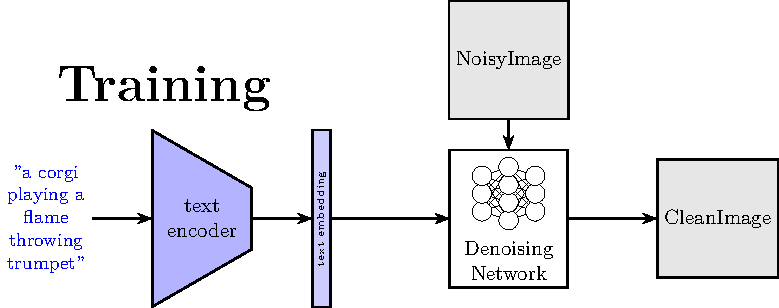
\includegraphics[width=\linewidth]{\toplevelprefix/chapters/chapter6/figs/tti-train.pdf}
    \caption{}
    % \label{}
  \end{subfigure}
  \hfill
  \begin{subfigure}{0.47\textwidth}
    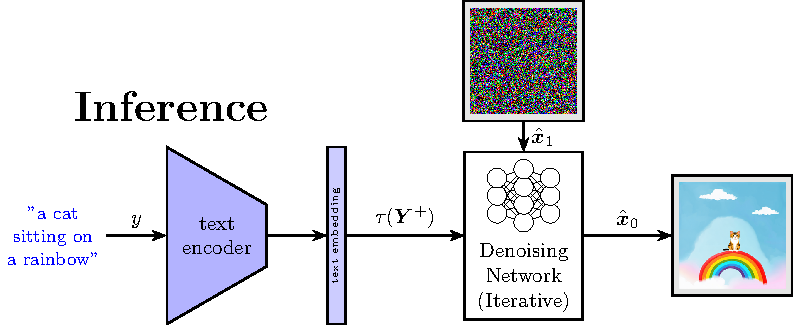
\includegraphics[width=\linewidth]{\toplevelprefix/chapters/chapter6/figs/tti-inf.pdf}
    \caption{}
    % \label{}
  \end{subfigure}
  % 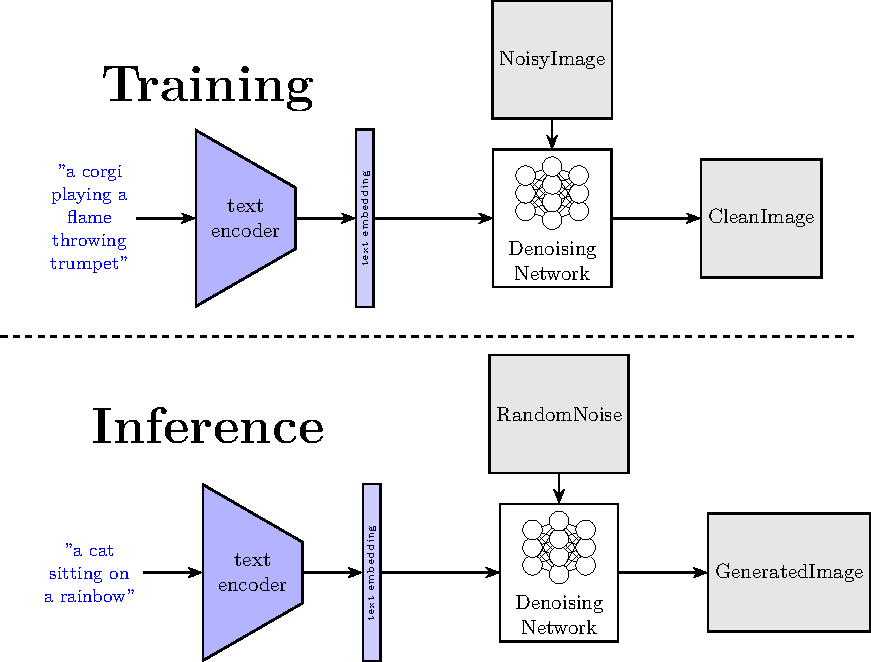
\includegraphics[width=0.8\linewidth]{\toplevelprefix/chapters/chapter6/figs/tti.pdf}

  \caption{训练和应用文本到图像生成模型的高层示意图,通过文本提示进行条件生成。\textbf{左图:}为了训练一个文本到图像模型,使用了一个大型的图像与相应文本标题配对的数据集。一个编码器被用来将标题映射到向量序列,这些向量序列被用作条件去噪器的条件信号,如 \Cref{sub:cfg} 中所述进行训练。文本编码器可以是预训练并冻结的,也可以与去噪器联合训练。\textbf{右图:}在应用训练好的模型时,使用一个期望的文本提示作为条件,然后用训练好的模型进行采样,如 \Cref{alg:iterative_denoising_conditional_CFG} 中所示(\textit{mutatis mutandis},稍作修改以用于编码后的文本提示)。有关将文本编码为向量序列过程的全部细节,请参见 \Cref{sec:clm_text}。}
  \label{fig:text-to-image}
\end{figure}

Stable Diffusion 遵循我们在 \Cref{sub:cfg} 中概述的条件生成方法,但有两个关键修改:(i)条件信号是分词后的文本提示 $\vY$,而不是类别标签;(ii)图像去噪是在“潜”空间中进行的,而不是在原始像素上,使用的是一个专门的、预训练的变分自编码器对 $f : \bR^{D_{\mathrm{img}}} \to \bR^{d_{\mathrm{img}}}$,$g : \bR^{d_{\mathrm{img}}} \to \bR^{D_{\mathrm{img}}}$(见 \Cref{sec:vae}),其中 $f$ 是编码器,$g$ 是解码器。随后的模型发展表明,第(ii)点是一个效率问题,而不是核心概念问题,所以我们不会重点关注它,只是提一下它只是导致对 \Cref{fig:text-to-image} 中勾勒的文本到图像流程进行以下直接修改:
\begin{enumerate}
  \item \textbf{在训练时},编码器 $f : \vx \mapsto \vz$ 被用来生成去噪目标,所有的去噪都在编码后的表示 $\vz_t \in \bR^{d_{\mathrm{img}}}$ 上进行;
  \item \textbf{在生成时},采样在表示 $\hat{\vz}_t$ 上进行,最终的图像通过应用解码器 $g(\hat{\vz}_0)$ 生成。
\end{enumerate}
相比之下,问题(i)是至关重要的,为处理它而提出的方法代表了 \textcite{rombach2022high} 的持久方法论创新之一。
在我们于 \Cref{sub:cfg} 中发展的迭代条件去噪框架的背景下,这涉及到去噪器 $\bar{\vz}_{\theta}(t, \vz_t, \vY^+)$ 的参数化。\footnote{在文本条件的设置中,“增强”标签 $\vY^+$,它要么是编码后的文本提示,要么是表示无条件去噪的 $\varnothing$,通常通过将 $\varnothing$ 映射到空字符串“”,然后像往常一样用分词器对这个文本提示进行编码来实现。这为处理文本条件的条件和无条件去噪提供了一种简单、统一的方法。}
\textcite{rombach2022high} 使用一种称为交叉注意力的层在去噪器中实现文本条件,其灵感来自 \textcite{vaswani2017attention} 的原始编码器-解码器 transformer 架构。交叉注意力的实现如下。我们让 $\tau : \bR^{D_{\mathrm{text}} \times N} \to \bR^{d_{\mathrm{model}} \times N_{\mathrm{text}}}$ 表示文本嵌入的编码网络(通常是一个因果 transformer——见 \Cref{sec:clm_text}),让 $\psi : \bR^{d_{\mathrm{img}}} \to \bR^{d_{\mathrm{model}} \times N_{\mathrm{img}}}$ 表示对应于去噪器中某个中间表示的映射。\footnote{在实践中,文本条件的去噪器在去噪器的前向传播中定期添加交叉注意力层,所以 $\psi$ 应被视为层依赖的,而 $\tau$ 则不是。详情请见 \textcite{rombach2022high}。} 这里,$N_{\mathrm{text}}$ 是最大分词文本提示长度,$N_{\mathrm{img}}$ 大致对应于表示中的图像通道数(层依赖),如果输入图像分辨率固定,则该值是固定的。交叉注意力(有 $K$ 个头,无偏置)定义为
    \begin{equation}
      \mathrm{MHCA}(\vz_t, \vY^+) \label{eq:mhca}
        = \vU_{\out}\mat{\SA([\vU_{\query}^{1}]^{\top}\psi(\vz_t),
        [\vU_{\rm key}^{1}]^{\top}\tau(\vY^+), [\vU_{\val}^{1}]^{\top}\tau(\vY^+)) \\ \vdots \\
        \SA([\vU_{\query}^{K}]^{\top}\psi(\vz_t),
        [\vU_{\rm key}^{K}]^{\top}\tau(\vY^+),
        [\vU_{\val}^{K}]^{\top}\tau(\vY^+))},
    \end{equation}
其中 $\mathrm{SA}$ 表示 transformer 中无处不在的自注意力操作(我们在 \Cref{ch:applications} 中详细回顾:见 \Cref{eq:mhsa,eq:self_attention}),而 $\vU_{*}^{k} \in \bR^{d_{\mathrm{model}}\times d_{\mathrm{attn}} }$ 对于 $* \in \set{\mathrm{qry}, \mathrm{key}, \mathrm{val}}$(以及输出投影 $\vU_{\mathrm{out}}$)是该层的可学习参数。

注意,根据自注意力操作的定义,交叉注意力\textit{输出的是值投影文本嵌入的线性组合,其权重由图像特征和文本嵌入之间的相关性决定。}
在 \textcite{rombach2022high} 使用的去噪器架构中,应用于当前层图像表示的自注意力残差块(其定义类似于视觉 transformer 的 \Cref{eq:vit-res-block} 中的那些)之后,是形式为 \eqref{eq:mhca} 的交叉注意力残差块。
这样的结构要求文本编码器 $\tau$ 在某种意义上,其输出与图像特征嵌入 $\psi$ 共享某些结构:这可以通过适当的联合文本-图像预训练(如使用 CLIP \cite{Radford2021-ir})或与去噪器本身联合训练来强制实现(后者由 \textcite{rombach2022high} 提出并展示,但由于高性能所需的高数据和训练成本而不再受欢迎)。
从概念上讲,这个联合的文本-图像嵌入空间和交叉注意力层本身与我们在上一节中推导的条件高斯混合去噪器(回顾 \eqref{eq:mog-conditional-denoising-unified-operator})在单个令牌序列的特殊情况下有很强的相似性。在多令牌设置中,可以遵循用于推导深度网络架构的率减框架(在 \Cref{ch:unrolling} 中讨论),并在 CRATE transformer 类架构的推导中体现出来,从而建立更深的联系。

这同一个基本设计已被进一步扩展到更大的模型和数据集规模,特别是在 Stable Diffusion 的现代实例 \cite{DBLP:conf/icml/EsserKBEMSLLSBP24} 中,以及在诸如 FLUX.1 \cite{Labs2025-fb}、Imagen \cite{Saharia2022-na} 和 DALL-E \cite{Ramesh2022-nu} 等竞争模型中。
交叉注意力的条件机制也已在其他应用中变得无处不在,如在 EgoAllo (\Cref{sub:ego-allo}) 中。


% \begin{itemize}
%   \item Embed image and text in a common space. (Embeddings, CLIP, reference
%     ch7)
%   \item Diffusion model to generate the images. Using CLIP. How to train it.
%   \item How to parameterize the denoiser. Cross-attention discussion, comparison
%     to the example.
%   \item Other stuff (``prior'', which maps from CLIP text embeddings to CLIP
%     image embeddings. Because the model maps from a CLIP image embedding to its
%     corresponding image (also conditioned on text). )
% \end{itemize}
%
% An vignette for image generation conditioned on a given caption.  \sdb{TODO:
% Discuss the cross-attention-type operator here. Can get it by considering
% a joint denoising of $p(x, y)$, with Gaussian conditional models for $p(y \mid
% x)$ and $p(x \mid y)$...}

% \sdb{Align Visual Data with Texts such as CLIP, with other attributes ControlNet, ... discuss dhariwal and nichol (classifier aware guidance), then mention DALLE type architecture for
% text-conditioned image generation?} \yima{Actually the original work ``\href{https://arxiv.org/abs/2105.05233}{Diffusion Models Beat GANs on Image Synthesis}'', by Prafulla Dhariwal and Alex Nichol, proposed to compute the two matching functions proposed above. The follow-up work ``Classifer-Free Diffusion Guidance''  by
% Jonathan Ho and Tim Salimans tried to simplify this by training the two matching functions together with one network with different condition inputs. We should feature those works here. However, we can mention that the large-scale realization DALLE, with a learned joint image-text binding by CLIP, adopts a somewhat heuristic way to realize the conditioning. So were many other follow-up works such as the ControlNet etc. ...}



\section{基于测量自洽性的条件推断}
\label{sec:measurement-self-consistency}
在本节的最后,我们考虑一个更极端但实际上普遍存在的分布学习情况,即我们只有一组观测到的数据样本 $\Y = \{\y_1,\ldots, \y_N\}$,而没有 $\x$ 的直接样本!通常,观测 $\y \in \mathbb{R}^d$ 的维度低于 $\x \in \mathbb{R}^D$。为了使问题明确,我们确实假设 $\y$ 和 $\x$ 之间的观测模型已知属于某个解析模型族,表示为 $\y = h(\x, \theta) +\vw$,其中 $\theta$ 可能已知或未知。

让我们首先通过一个简单的案例来从概念上理解这个问题,即当测量函数 $h$ 已知且观测到的 $\y = h(\x) + \vw$ 对 $\x$ 具有信息量时。也就是说,我们假设 $h$ 是从 $\x$ 的空间到 $\y$ 的空间上的满射,并且分布 $\y_0 = h(\x_0)$ 的支撑集是低维的。这通常要求 $\y$ 的\textit{外在}维度 $d$ 高于 $\x$ 分布支撑集的\textit{内在}维度。不失一般性,我们可以假设存在函数:
\begin{equation}
F(\x) = \boldsymbol{0},\quad     G(\y) = \boldsymbol{0}.
\end{equation}
注意,这里我们可以假设我们知道 $G(\y)$ 但不知道 $F(\x)$。设 $\mathcal{S}_{\y} \doteq \{\y \mid G(\y) = \boldsymbol{0}\}$ 为 $p(\y)$ 的支撑集。通常,$h^{-1}(\mathcal{S}_{\y}) = \{\x \mid G(h(\x)) = \boldsymbol{0}\}$ 是 $\mathcal{S}_{\x} \doteq \{\x \mid F(\x) = \boldsymbol{0}\}$ 的一个超集。也就是说,我们有 $h(\mathcal{S}_{\x}) \subseteq \mathcal{S}_{\y}$。

% \paragraph{Geometric Interpretation via Constrained Optimization.}
% Now given $\vnu = h(\x) + \vw$, to solve for $\x$, we can solve the following constrained optimization problem:
% \begin{equation}
%     \max_{\x} - \frac{1}{2}\|h(\x) - \vnu\|_2^2 \quad \mbox{s.t.} \quad G(h(\x)) = \boldsymbol{0}. 
% \end{equation}
% Using augmented Lagrange multiplier method, we can solve the following unconstrained program:
% \begin{equation}
%    \max_{\x} -\frac{1}{2}\|h(\x) - \vnu\|_2^2  + \vlambda^TG(h(\x)) -  \frac{\mu}{2} \|G(h(\x)) \|_2^2,
% \end{equation}
% for some Lagrange multipliers. This is equivalent to the following program:
% \begin{equation}
% \max_{\x} = \log\exp\Big(- \frac{1}{2}\|h(\x) - \vnu\|_2^2\Big)  + \log \exp\Big( - \frac{\mu}{2} \|G(h(\x)) - \vlambda/\mu\|_2^2\Big),
% \end{equation}
% for some vector $\vc = \vlambda/\mu$. That is, the augmented Lagrange multiplier method that enforces the constraint $G(\y) = \boldsymbol{0}$ is equivalent to use the score function of the probability density:
% \begin{equation}
%     p(\y) = \exp\Big( - \frac{\mu}{2}\|G(\y) - \vc\|_2^2\Big).
% \end{equation}


\subsection{线性测量模型}
首先,为简单起见,我们考虑测量是我们所关心的数据 $\x$ 的一个线性函数:
\begin{equation}
    \y = \vA\x.
\end{equation}
这里矩阵 $\vA \in \mathbb{R}^{m\times n}$ 是行满秩的,且 $m$ 通常小于 $n$。我们暂时假设 $\vA$ 是已知的。我们感兴趣的是如何从这样的测量中学习 $\x$ 的分布。由于我们不再有 $\x$ 的直接样本,我们想知道是否仍然可以为 $\x$ 开发一个去噪器,仅使用观测 $\y$。让我们考虑以下扩散过程:
\begin{equation}
    \y_t = \y_0 + t \vg, \quad \y_0 = \vA(\x_0), 
\end{equation}
其中 $\vg \sim \mathcal{N}(\boldsymbol{0}, \vI)$。

% \paragraph{Having access to the diffusion process $\x_t$.}
% Let us first consider the following diffusion process:
% \begin{equation}
%     \x_t = \x_0 + \sigma_t \vg, \quad \y_t = \vA(\x_t), 
% \end{equation}
% where $\vg \sim \mathcal{N}(\boldsymbol{0}, \vI)$. 
% Then one show that 
% \begin{equation}
%     \hat{\x}_* = \argmin \mathbb{E}[\|\vA(\hat{\x}(\vA\x_t, \vA) - \x_0)\|^2]
% \end{equation}
% satisfies the condition that:
% \begin{equation}
%     \vA \hat{\x}_*(\vA\x_t, \vA) = \vA \mathbb{E}[\x_0 \mid \vA \x_t, \vA].
% \end{equation} Notice that in the special case when $\vA$ is of  full column rank, we have $ \mathbb{E}[\x_0 \mid \vA\x_t, \vA] = \mathbb{E}[\x_0 \mid \x_t]$. Hence, in the more general case, it was suggested in the work \cite{daras2023ambient} that one could still use the so obtained $\mathbb{E}[\x_0 \mid \vA\x_t, \vA]$ to replace the $\mathbb{E}[\x_0 \mid \x_t]$ in the normal denoising process. This usually works very well in practice, say for many image restoration tasks.

% However, one should notice that the above process relies on the assumption that we have access to samples of the diffused distribution of $\x_t$, in an order to learn the denoiser $\mathbb{E}[\x_0 \mid \vA\x_t, \vA]$. That is often not the case in practice when we only have samples of the measurement $\y$ and its diffusion process $\y_t$. 
% \yima{Druv, actually, I think the above so-called ambient diffusion is more related to the measurement matching case studied in Subsection 2, where we train a masked auto-encoder...}

不失一般性,我们假设 $\vA$ 是行满秩的,即欠定的。我们定义相应的过程 $\x_t$ 为满足以下条件的过程:
\begin{equation}
\y_t = \vA \x_t.   
\end{equation}

从 $\y_t$ 的去噪过程中,我们有
\begin{equation}
    \y_{t-s} \approx  \y_t + st \nabla \log p_t(\y_t).
\end{equation}
那么我们有:
\begin{equation}
    \vA\x_{t-s} \approx   \vA\x_t + st \nabla \log p_t(\vA \x_t),
\end{equation}
对于一个小的 $s >0$。所以 $\x_{t-s}$ 和 $\x_t$ 需要满足:
\begin{equation}
    \vA(\x_{t-s} - \x_t) \approx st \nabla \log p_t(\vA\x_t). 
\end{equation}
在所有满足上述约束的 $\x_{t_s}$ 中,我们任意选择最小化距离 $\|\x_{t-s} - \x_t\|_2^2$ 的那一个。因此,我们得到了一个针对 $\x_t$ 的“去噪”过程:
\begin{equation}
    \x_{t-s}  \approx \x_t + st\vA^\dagger \nabla \log p_t(\vA\x_t). 
\label{eqn:denoising-projection}
\end{equation}
注意,这个过程并不是从 $\vx_t$ 的分布中采样。特别是,$\vA$ 的零空间/核中的 $\vx$ 的分量永远无法从观测中恢复。因此,严格来说,需要更多信息才能恢复 $\vx$ 的完整分布。但这恢复了与 $\vA$ 的零空间正交的 $\vx$ 的分量。

% \paragraph{Inference.}
% Notice that the above process is trying to enforce the constraints learned for the low-dimensional distribution of $\y$. Given a specific observation of $\y = \vnu$, to solve the inverse problem of inferring $\x$, we also want to enforce the measurement constraint $\vnu = \vA \x$, say through the gradient descent of $\frac{1}{2} \|\vA \x_t - \vnu\|_2^2$:
% \begin{equation}
%     \x_{t-s} = \x_t + s \vA^\dagger (\vnu - \vA \x_t).
% \end{equation}
% Combining the two terms we obtain an iterative process for $\x_t$:
% \begin{equation}
%     \x_{t-s} = \x_t + s \vA^\dagger\big[t \nabla \log p_t(\vA \x_t) +  (\vnu - \vA \x_t)\big].
% \end{equation}

% \paragraph{The Over-determined Case.}
% Now let us consider the case when $\vA$ is over-determined. We may define the process $\x_t$ by 
% \begin{equation}
% \x_t = \argmin_{\x} \|\vA \x - \y_t\|^2 = \vA^\dagger \y_t.
% \end{equation}
% From the denoising process for $\y_t$, we have
% \begin{equation}
%    \vA^\dagger \y_{t-s} =  \vA^\dagger\y_t + st \vA^\dagger \nabla \log p_t(\y_t).
% \end{equation}
% Since $\x_t = \vA^\dagger \y_t$ and $\vA \x_t = \vA\vA^\dagger \y_t$, we have
% \begin{equation}
%     \x_{t-s}  \approx \x_t + st\vA^\dagger \nabla \log p_t(\vA\x_t),
% \label{eqn:denoising-lifting}
% \end{equation}
% where for the score function $\nabla \log p_t(\y_t)$, we only care about how to denoise $\y_t$ in the range of $\vA$.

% We may consider the following estimate
% \begin{equation}
%     \hat{\x}_*(\y_t) = \argmin \mathbb{E}[\|\y_t - \vA\x_0)\|^2]
% \end{equation}


\subsection{从已标定的图像对学习三维视觉模型}
在实践中,测量模型通常是非线性的或仅部分已知。这类问题的一个典型例子实际上是我们如何从感知的图像(例如通过我们的眼睛、望远镜或显微镜)中学习外部世界的工作模型。特别是,人类和动物能够通过一系列二维投影——即一系列二维图像(或立体图像对)——建立一个三维世界(或动态世界的四维)模型。投影的数学或几何模型通常是已知的:
\begin{equation}
    \y^i = h(\x, \theta^i) +\vw^{i}, 
\end{equation}
其中 $h(\cdot)$ 表示在某个相机视角 $t_i$ 下,三维(或四维)场景到二维图像(或立体对)的(透视)投影,而 $\vw$ 是某种可能为加性的小测量噪声。\Cref{fig:projection-2D} 具体说明了这种关系,而 \Cref{fig:inference_distributed} 则抽象地说明了这个问题模型。关于三维场景的多个二维视图相关的几何学的完整阐述超出了本书的范围。感兴趣的读者可以参考书籍 \cite{MaY2003}。目前,我们继续所需要的只是,这样的投影是众所周知的,并且一个场景的多个图像包含了关于该场景的足够信息。
\begin{figure}[t]
    \centering
    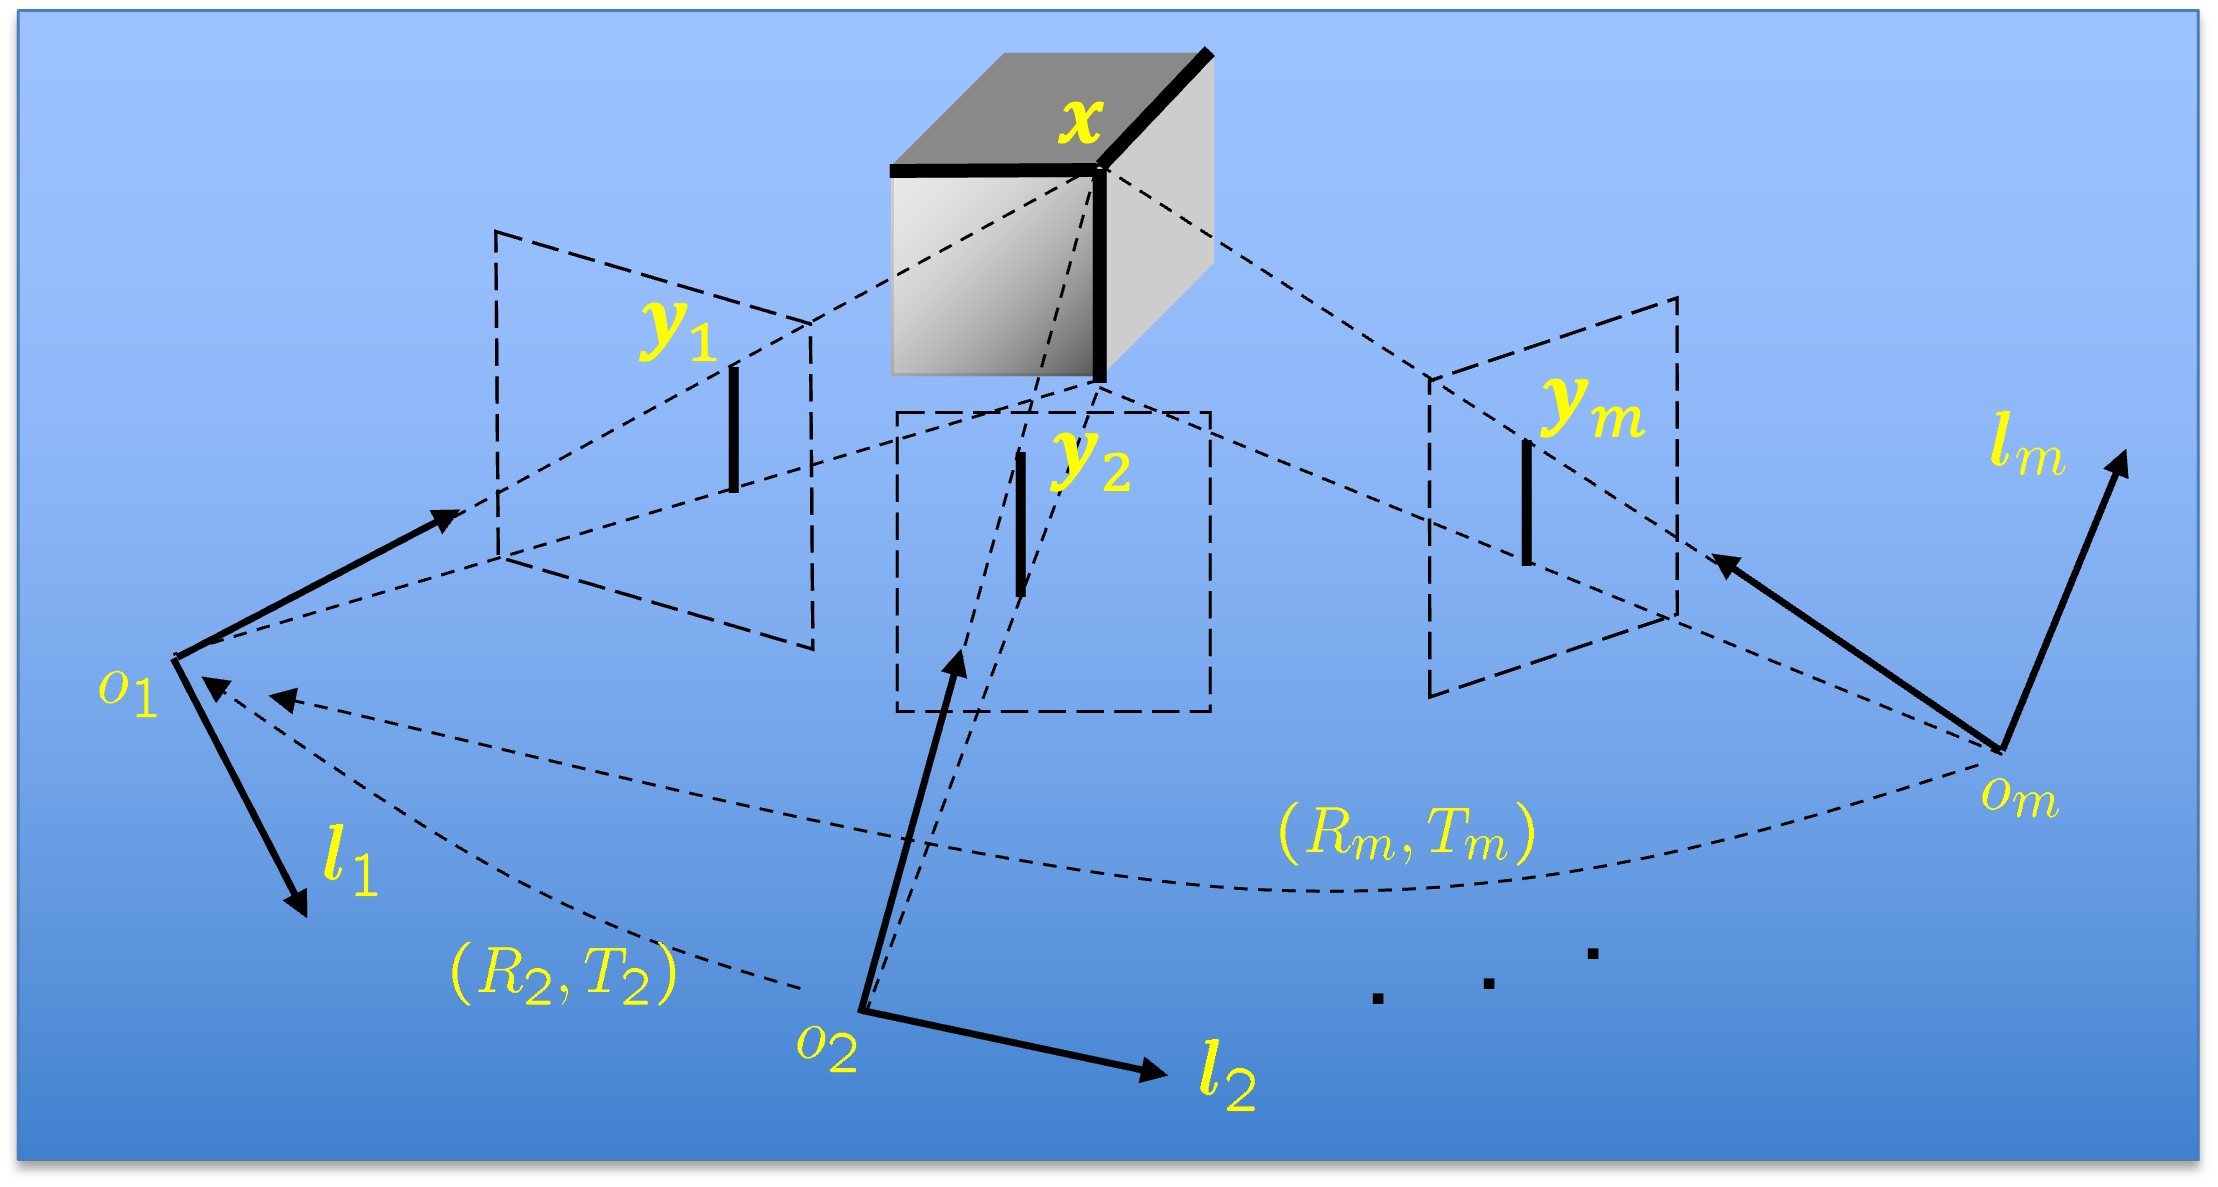
\includegraphics[width=0.7\linewidth]{\toplevelprefix/chapters/chapter6/figs/3D-2D-projection.png}
    \caption{三维物体/场景与其二维投影之间的关系。这里我们展示了一个点 $\x$ 和一条与该点相交的线的投影。}
    \label{fig:projection-2D}
\end{figure}

\begin{figure}[t]
  \centering 
  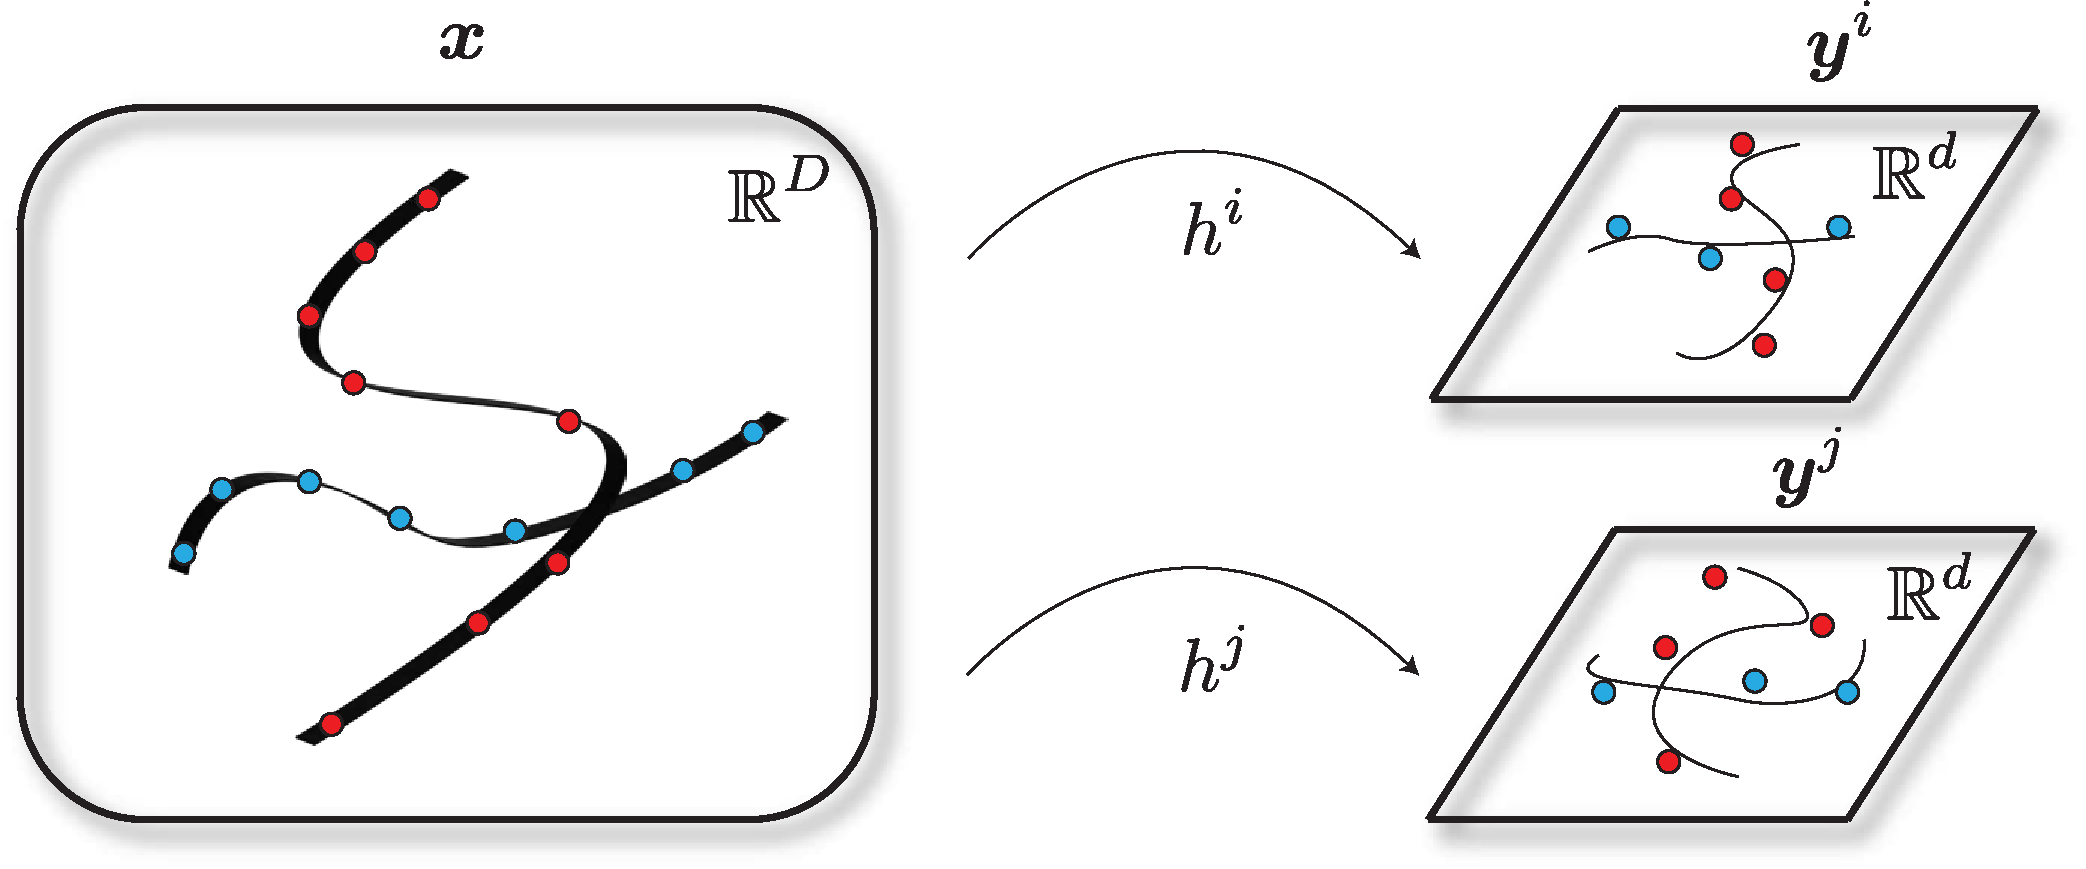
\includegraphics[width=0.7\linewidth]{\toplevelprefix/chapters/chapter6/figs/inference_distributed.pdf}
  \caption{\small \textbf{基于分布式测量的推断。} 我们有一个低维分布 \(\vx\)(这里,与 \Cref{fig:inference_roadmap} 类似,描绘为 \(\R^{3}\) 中两个二维流形的并集)和一个测量模型 \(\y^{i} = h^{i}(\vx) + \vw^{i}\)。和之前一样,我们希望推断给定 \(\vy\) 时 \(\vx\) 的条件分布的各种性质,其中 \(\vy\) 是所有测量 \(\y^{i}\) 的集合。}
  \label{fig:inference_distributed}
\end{figure}

通常,我们希望从迄今为止感知到的世界的二维图像中学习三维(或四维)世界场景 $\x$ 的分布 $p(\x)$。\footnote{这里,为了方便,我们使用 $\x$ 来表示三维空间中的一个点,或者一个由许多点组成的完整三维物体或场景的样本。} 这样一个(视觉)世界模型的主要功能是让我们能够识别我们曾经去过的地方,或者预测当前场景在未来的某个时间点从一个新的视角看会是什么样子。

让我们首先考察立体视觉这个特殊但重要的案例。在这种情况下,我们有两个关于三维场景 $\x$ 的已标定视图:
\begin{equation}
    \y^0 = h(\x, \theta^0) +\vw^0, \quad \y^1 = h(\x, \theta^1) +\vw^1, 
\end{equation}
其中视图姿态的参数 $\theta_0$ 和 $\theta_1$ 可以假设是已知的。$\y^0$ 和 $\y^1$ 是三维场景 $\x$ 的两个二维投影。我们也可以假设它们具有相同的边缘分布 $p(\y)$,并且我们已经为其学习了一个扩散和去噪模型。也就是说,我们知道去噪器:
\begin{equation}
  \bE[\vy \mid \vy_t=\vnu] =
  \vnu + t^2 \nabla_{\vnu}\log p_t(\vnu). 
 \label{eq:y-posterior-sampling-denoiser}    
\end{equation}
或者,更进一步,我们可以假设我们有足够数量的立体对 $(\y^0, \y^1)$ 样本,并且也学习了这对样本的联合分布。为方便起见,我们也用 $\y = h(\x)$ 来表示这对 $\y = (\y^0, \y^1)$,并用 $p(\y)$ 表示这对样本学习到的概率分布(例如,通过上述的去噪器)。

现在的主要问题是:如何从两个已知关系的投影中学习三维场景 $\x$ 的分布(或其表示)?
% Or equivalently, how to learn a denoiser for $\x$
% \begin{equation}
%   \bE[\vx \mid \vx_t=\vxi] =
%   \vxi + t^2 \nabla_{\vxi}\log p_t(\vxi),
%  \label{eq:x-posterior-sampling-denoiser}    
% \end{equation}
% where we have $\vnu^0 = h(\vxi, \theta^0)$ and $\vnu^1 = h(\vxi, \theta^1)$.
人们可能会质疑这样做的理由:如果函数 $h(\cdot)$ 在很大程度上是可逆的,为什么这是必要的?也就是说,观测 $\y$ 可以在很大程度上确定未知的 $\x$,这对于立体视觉来说在某种程度上是成立的——通常,两个(已标定的)图像包含关于场景深度的足够信息,从给定的有利位置来看。然而,二维图像远非三维场景最紧凑的表示,因为同一个场景可以产生无限多个(高度相关的)二维图像或图像对。事实上,一个好的三维场景表示应该是对视点不变的。因此,一个正确的三维场景分布表示应该比二维图像、立体对或图像-深度对的分布更紧凑和结构化。

考虑在 \eqref{eq:y-posterior-sampling-denoiser} 中扩散过程 $\y_t = \y + t\vg $ 的(逆)去噪过程,其中 $\vg$ 是标准高斯分布。从 \eqref{eq:y-posterior-sampling-denoiser} 的去噪过程中,我们有
\begin{equation}
    \y_{t-s} =  \y_t + st \nabla_{\y} \log p_t(\y_t).
\end{equation}
我们试图找到一个对应的 $\x_t$ 的“去噪”过程,使得 $\x$ 与 $y$ 的关系为:
\begin{equation}
    \y =  h(\x).
\end{equation}

那么我们有:
\begin{equation}
    h(\x_{t-s}) \approx  h(\x_t) + st \nabla_{\y} \log p_t(h(\x_t)),
\end{equation}
对于一个小的 $s >0$。
% We then can iteratively solve for $\x_{t-s}$ from
% \begin{equation}
%     \hat{\x}_{t-s} = \argmin_{\z} \|h(\z) - h(\x_t) - st \nabla \log p_t(h(\x_t))\|_2^2.
% \end{equation}
假设 $\x_{t-s} = \x_t + s \vv$ 对于某个向量 $\vv$ 和小增量 $s$。我们有
\begin{equation}
    h(\x_{t-s}) \approx h(\x_t) + \frac{\partial h}{\partial \x}(\vx_{t}) \cdot \vv s \doteq h(\x_t) + \vA(\x_t) \vv s. 
\end{equation}
因此,我们有
\begin{equation}
    \vA(\x_t) \vv = t \nabla_{\y} \log p_t(h(\x_t)).
    \label{eqn:pushforward}
\end{equation}
几何上,$\x$ 域中的向量 $\vv$ 可以被看作是向量场 $t \nabla \log p_t(\y)$ 在映射 $\y = h(\x)$ 下的拉回。通常,和之前一样,我们可以(任意地)选择 $\vv$ 为满足拉回关系的最小 2-范数向量。因此,我们可以近似地将 $\hat{\x}_{t-s}$ 表示为:
\begin{equation}
    \hat{\x}_{t-s} \approx \x_t + st\vA(\x_t)^\dagger \nabla_{\y} \log p_t(h(\x_t)). 
\label{eqn:pullback-denoise}
\end{equation}


\begin{remark}[并行感知与分布式去噪]
{上述方程 \eqref{eqn:pullback-denoise} 中有一些非常有趣的地方。它似乎表明我们可以尝试通过一个与(许多)其(部分)观测耦合的过程来学习 $\x$ 的分布:
\begin{equation}
\y^i = h^i(\x) +\vw^i, i =1, \ldots, K.
\end{equation} 在这种情况下,我们得到了一组 $\x$ 域中向量场 $\vv$ 应满足的方程:
\begin{equation}
    \vA^i(\x_t) \vv = t \nabla_{\y^i} \log p_t(h^i(\x_t)),
\label{eqn:federated-pushforward}
\end{equation}
其中 $\vA^i(\x_t) = \frac{\partial h^i}{\partial \x}(\vx_t)$。最终的 $\vv$ 可以被选择为满足所有上述方程的“集中式”解,或者它可以被选择为所有 $\vv^i$ 的某种(随机的)“聚合”版本:
\begin{equation}
    \vv^i = t\vA^i(\x_t)^\dagger \big[\nabla_{\y^i} \log p_t(h^i(\x_t))\big], \quad i = 1, \ldots, K,
\end{equation}
这些是以并行和分布式的方式计算的?这里一个悬而未决的问题是,即使在线性测量模型的情况下,这样定义的 $\x_t$ 的“去噪”过程究竟会收敛到什么?当 $\y_t$ 收敛到 $\y = h(\x_0)$ 时,它何时会收敛到一个与原始 $\x_0$ 具有相同低维支撑集的分布? }
\end{remark}

% \paragraph{Inference.}
% Notice that the above process is to enforce the low-dimensional constraint for the support of $\y$. In the case when we like to conduct inference of $\x$ from an observation $\y = h(\x)$, we also need to enforce constraint on the measurement, say through gradient descent on $\frac{1}{2} \|h(\x) - \y\|_2^2$:
% \begin{equation}
%     \hat{\x}_{t-s} = \x_t + s \vA(\x_t)^\dagger (\y - h(\x_t)). 
% \end{equation}
% Hence together, we have the following iterative process for inferring $\x$:
% \begin{eqnarray}
%  \hat{\x}_{t-s} = \x_t + s \vA(\x_t)^\dagger\big[t \nabla_{\y} \log p_t(h(\x_t)) +  (\y - h(\x_t)) \big].   
% \end{eqnarray}
% Notice that when $h$ is linear, the above approximation reduces to the same form that we have obtained in the previous subsection. 


\paragraph{从未标定的图像序列学习视觉世界模型}

在上述推导中,我们假设测量模型 $h(\cdot)$ 是完全已知的。在立体视觉的情况下,这是相当合理的,因为两个相机视图(或两只眼睛\footnote{我们两只眼睛的相对姿态对我们的大脑来说是众所周知的。})的相对姿态(和标定)通常是预先知道的。因此,通过立体图像对,原则上我们应该能够学习三维场景的分布,至少是三维场景的自我中心分布。然而,所谓的学习到的分布的低维结构包含了由于改变视点而引起的变化。也就是说,当我们相对于同一个三维场景改变我们的视点时,立体图像的外观会发生变化。对于许多实际的视觉任务(如定位和导航),如果我们能将这种视点变化从三维场景的不变表示中解耦出来,那将非常重要。

\begin{remark}请注意,上述目标与克莱因的爱尔兰根纲领对现代几何学的目标非常吻合,即研究一个流形在一组变换下的不变量。在这里,我们可以将感兴趣的流形看作是三维场景的自我中心表示的分布。我们已经知道它允许一个三维刚体运动群作用于其上。值得注意的是,我们的大脑已经学会了有效地将这种变换与观测到的三维世界解耦。
\end{remark}


请注意,我们已经在第 \ref{ch:representation} 章中,在一个有限的设置下研究了学习对平移和旋转不变的表示。我们知道,相关的压缩算子必然采用(多通道)卷积的形式,从而导致(深度)卷积神经网络。然而,与更一般的变换群不变的压缩或去噪相关的算子仍然难以刻画 \cite{cohen2016group}。
对于最一般设置下的三维视觉问题,我们知道我们视点的变化可以很好地建模为刚体运动。然而,我们眼睛在不同视点之间的确切相对运动通常是未知的。更一般地,场景中也可能有物体(例如,汽车、人、手)在移动,而我们通常也不知道它们的运动。我们如何将用已标定的立体对学习三维场景分布的问题推广到这样更一般的设置?更精确地说,我们想要学习一个三维场景的紧凑表示 $\x$,它对相机/眼睛的运动是不变的。一旦学习了这样的表示,我们就可以采样并生成一个三维场景,并从任意姿态渲染图像或立体对。

% In fact, without specifying the ego-centric frame as the reference for each stereo pair, it might lead to a more compact representation of the 3D scene that is invariant to the ego-centric viewpoint (say, if the camera views are specified with respect to some canonical world frame of the scene). In fact, our brain seems to be able to learn such a representation that decouples objects in a 3D scene and the motion of the observer or the objects.

为此,注意到我们可以将一系列立体对建模为:
\begin{equation}
    \y^k = h(\x^k, \theta^k), \quad k=1, \ldots, K,
\end{equation}
其中 $h(\cdot)$ 表示从三维到二维的投影图。$\theta^k$ 表示第 $k$ 个视图的刚体运动参数,相对于世界中的某个规范坐标系。$\x^k$ 表示时间 $k$ 的三维场景。如果场景是静态的,$\x^k$ 应该都是相同的 $\x^k = \x$。为了简化符号,我们可以将这 $k$ 个方程的集合表示为一个:
\begin{equation}
    \Y = H(\x,\Theta). 
\end{equation}
我们可以假设我们被给予了许多这样的立体图像序列 $\{\Y_i\}$ 的样本。问题是如何恢复相关的运动序列 $\{\Theta_i\}$ 并学习场景 $\x$ 的分布(该分布对运动是不变的)。据我们所知,这仍然是一个悬而未决的挑战性问题,可能是三维视觉问题的最后前沿。

% Now suppose we have learned the distribution $p(\y)$ of the ego-centric stereo pairs $\y$ via a denoisng process $\y_t \sim p_t$. Similar as before, we associate a process $(\x_t, \Theta)$ with $\Y_t$ as:
% \begin{equation}
%     \Y_t \approx H(\x_t, \Theta). 
% \end{equation}

% Heuristically, we then can iteratively solve for $\x_{t-s}$ from
% \begin{equation}
%     (\hat{\x}_{t-s}) = \argmin_{\z} \|H(\z, \Theta) - H(\x_t, \Theta) - st \nabla \log p_t(H(\x_t,\Theta))\|_2^2.
% \end{equation}
% Suppose $\z = \x_t + \Delta \x$ for some small increment. We have
% \begin{equation}
%     H(\z, \Theta) \approx H(\x_t, \Theta) + \frac{\partial H}{\partial \z}\bigg\rvert_{\x_t, \Theta} \Delta \x  \doteq H(\x_t,\Theta) + \vA \Delta \x. 
% \end{equation}
% Given an estimate of $\x_t$, we also would like to enforce better measurement consistency by optimizing $\Theta$ through
% \begin{equation}
%     \min_{\Theta} \frac{1}{2}\|H(\x_t, \Theta) - \Y\|_2^2.
% \end{equation}

% Hence, we can solve for $\hat{\X}_{t-s}, \hat{\Theta}_{t-s}$ in an iterative and alternating fashion:
% \begin{eqnarray}
%     \hat{\Theta}_{t-s} &\approx& \Theta_t +  s \vB^\dagger\big[\Y - H(\x_{t}, \Theta_t)\big], \quad \quad \quad \vB = \frac{\partial H}{\partial\Theta}\bigg\rvert_{\x_t, \Theta_t},\\
%     \hat{\x}_{t-s} &\approx& \x_t + s \vA^\dagger\big[t  \nabla \log p_t(H(\x_t, \Theta_{t-s}))  \big], \quad \vA = \frac{\partial H}{\partial \z}\bigg\rvert_{\x_t, \Theta_{t-s}}.
% \end{eqnarray}
% \yima{Under what conditions, the learned denoiosing process for $\x$ can be invariant to the motions of the viewpoints?}


\section{总结与注释}
\paragraph{无干净样本的测量匹配。} 在我们对条件采样的发展中,我们考虑了在观测模型 \eqref{eq:measurement-matching-observation} 下的测量匹配,其中我们假设我们有配对数据 $(\vx, \vy)$——即每个观测 $\vy$ 都有真实值。
在许多实际相关的逆问题中,情况并非如此:最基本的例子之一是在压缩感知的背景下,我们回顾了 \Cref{ch:classic},其中我们需要利用关于 $\vx$ 的先验知识(即稀疏性)从 $\vy$ 重建 $\vx$。
在去噪-扩散的设置中,我们通过学习到的去噪器 $\bar{\vx}_{\theta}(t, \vxi)$ 获得了 $\vx$ 的隐式先验。我们是否仍然可以在没有真实样本 $\vx$ 的情况下进行条件采样?

为了直观地理解为什么这可能是可能的,我们回顾一个统计学中的经典例子,称为斯坦无偏风险估计(SURE)。
在观测模型 $\vx_t = \vx + t \vg$ 下,其中 $\vg \sim \cN(\Zero, \vI)$ 且 $t>0$,事实证明,对于任何弱可微的 $f : \bR^D \to \bR^D$,
\begin{equation}\label{eq:sure-risk}
  \bE_{\vg}\left[
    \norm*{\vx - f(\vx + t \vg)}_2^2
    \right]
  =
  \bE_{\vg}\left[
    \norm*{\vx+t\vg - f(\vx + t \vg)}_2^2
    + 2t^2 \nabla \cdot f(\vx + t\vg)
    \right]
  - t^2 D,
\end{equation}
其中 $\nabla \cdot$ 表示散度算子:
\begin{equation*}
	\nabla \cdot f = \sum_{i=1}^D \partial_i f_i.
\end{equation*}
\Cref{eq:sure-risk} 右侧的依赖于 $\vx$ 的部分被称为斯坦无偏风险估计(SURE)。如果我们在 \Cref{eq:sure-risk} 中对 $\vx$ 取期望,注意右侧可以写成关于 $\vx_t$ 的期望——特别地,\textit{任何去噪器 $f$} 的均方误差都可以\textit{仅从带噪样本中估计}!
这个非凡的事实,以精炼的形式,构成了许多仅使用带噪数据进行图像恢复、去噪-扩散等实用技术的基础:著名的例子包括“noise2noise”范式 \cite{pmlr-v80-lehtinen18a} 和 Ambient Diffusion \cite{daras2023ambient}。

作为一个有趣的旁注,我们指出 \Cref{eq:sure-risk} 导致了特威迪公式(\Cref{thm:tweedie})的另一种证明。从高层次看,我们对 $\vx$ 取期望,并通过分部积分将 \Cref{eq:sure-risk} 右侧的主要部分等价地表示为
\begin{equation}
  \bE_{\vx_t}\left[
    \norm*{\vx_t - f(\vx_t)}_2^2
    + 2t^2 \nabla \cdot f(\vx_t)
    \right]
  =
  \bE_{\vx_t}\left[
    \norm*{\vx_t - f(\vx_t)}_2^2
    \right]
  - 2t^2 \int
  \ip*{\nabla p_{\vx_t}(\vxi)}{f(\vxi)}
  \odif \vxi.
\end{equation}
这是一个关于 $f$ 的二次函数,形式上求导可以得出最优的 $f$ 满足特威迪公式(\Cref{thm:tweedie})。这个论证可以使用变分法的基本思想来使其严谨。


\paragraph{对扩散后验采样(DPS)近似的修正。}
在 \Cref{example:denoising-conditional-gaussian} 中,特别是在 \Cref{fig:conditional_sampling_computational_gaussian} 中,我们指出了 DPS 近似 \Cref{eq:conditional-posterior-measurementmatching-gaussian-case-dps-approx} 在小测量噪声水平下的一个局限性。
这个局限性已得到充分理解,Rozet 等人 \cite{rozet2024learning} 提出了一种有原则的改进方法。
该方法涉及在 \Cref{eq:conditional-posterior-measurementmatching-gaussian-case-dps-approx} 中加入对带噪后验 $p_{\vx \mid \vx_t}$ 方差的额外估计——详情请参阅该论文。
对后验方差的自然估计比 DPS 本身的可扩展性稍差,因为需要对后验去噪器 $\bE[\vx \mid \vx_t=\vxi]$ 的雅可比矩阵(一个大矩阵)的仿射变换求逆。Rozet 等人 \cite{rozet2024learning} 使用自动微分和基于共轭梯度的逆近似相对高效地完成了这一步。似乎应该有可能在此方法的基础上进一步改进(例如,使用二阶优化的经典思想)。


\paragraph{关于测量匹配和用于逆问题的扩散模型的更多信息。}

扩散模型已成为解决科学应用中出现的逆问题的极其流行的工具。除了我们在 \Cref{alg:iterative_denoising_conditional_DPS} 中介绍的简单 DPS 算法之外,已经开发并正在继续开发更多的方法,因为该领域正在迅速发展。
除 DPS 外,流行且性能优越的方法类别包括变量分裂方法,如 DAPS \cite{Zhang2024-ha},它允许比 DPS 更强地强制执行特定的测量约束,以及可以避免使用像 DPS 中那样的近似的精确方法,如 TDS \cite{wu2023practical}。
关于该领域的更多信息,我们推荐 \cite{zheng2025inversebench},它既是一篇综述,也是对几种流行方法在特定科学逆问题数据集上的基准测试。

\section{练习}

\begin{exercise}[对DPS的后验方差校正]

\begin{enumerate}
\item 使用本书GitHub中提供的代码实现\Cref{fig:conditional_sampling_computational_gaussian},并实现\textcite{rozet2024learning}提出的后验方差校正。
\item 验证该方法是否改善了在\Cref{fig:conditional_sampling_computational_gaussian}中观察到的低噪声方差下的后验坍塌问题。
\item 讨论校正方法保留或引入的任何采样正确性问题,以及其相对于扩散后验采样(DPS)的效率。
\end{enumerate}

\end{exercise}

\begin{exercise}[在MNIST上的条件采样]
\begin{enumerate}
\item 为MNIST数据集训练一个简单的分类器,架构自选。此外,训练一个适用于条件采样的去噪器(\Cref{alg:iterative_denoising_conditional_CFG},因为该去噪器也可用于无条件去噪)。
\item 将分类器集成到基于分类器指导的条件采样器中,如\Cref{sub:cfg}第一部分所述。从与条件类别的保真度(视觉上;根据最近邻;根据分类器的输出)方面评估生成的样本。
\item 将分类器集成到基于无分类器指导的条件采样器中,如\Cref{sub:cfg}和\Cref{alg:iterative_denoising_conditional_CFG}所述。执行与上一步相同的评估,并比较结果。
\item 在CIFAR-10数据集上重复该实验。
\end{enumerate}

\end{exercise}


\end{document}
